This chapter elaborates on the power budget and requirements leading to the proposed solar array design. Reference Sols and their rover modes are defined in \refSec{sec:Design:ReferenceSols} so that mission scenario power budgets may be formalized in \refSec{sec:Design:PowerBudget}. Particular attention is put on analyzing field trial data from which propulsion power draw requirements are extracted. \refSec{sec:Design:RequirementsAndDesignDrivers} consolidates assumptions, requirements, conwtraints, and design drivers that will guide the proposed design of the rover's \ac{PV} system. Solar array sizing and configurations as well as necessary rover body redesign are presented in \refSec{sec:Design:SolarArray}. A rudimentary simulation environment for solar power management is introduced in \refSec{sec:Design:Simulation} as a potential for future work before summarizing and concluding the chapter in \refSec{sec:Design:SummaryAndConclusion}.

\section{Reference Sols}
\label{sec:Design:ReferenceSols}
Baseline content for this section were taken from \citeother{CDF2014} and constrained to the scope of this thesis. Adjustements were made in relation to the mission sites described in the previous chapter as well as with the rover's capabilities with respect to its active suspension system. Rover modes were identified and then sequenced into high-level reference Sols for mission planning. Defining rover modes and reference Sols served as a prerequisite to formalizing power budgets by assignment each rover modes with their power draw and minimal operational duration.

%The chapter is structured as follows: Section \ref{sec:ReferenceSols:RoverModes} provides general definitions of rover modes. The identified rover modes are sequenced into reference Sols in Section \ref{sec:ReferenceSols:ReferenceSols}. The chapter is then summarized in Section \ref{sec:PowerBudget:SummaryAndConclusion}.

\subsection{Rover Modes}
\label{sec:ReferenceSols:RoverModes}
Not all modes defined in \citeother{CDF2014} were included in this section, however; they may become of interest in future design iterations. The omitted modes are \textit{Launch}, \textit{\ac{EDL}}, \textit{Deployment}, \textit{Science Stop - Long},  and \textit{Safe} modes. The rover modes considered in this thesis are as follow:

\begin{itemize}
    \item \textbf{Traverse - Flat:} Pre-planned flat surface traverses to target destinations.
    \item \textbf{Traverse - Upslope:} Pre-planned upslope surface traverses to target destinations.
    \item \textbf{Science Stop - Short:} Short science activities in between traverses.
    \item \textbf{\ac{DTE} Communication:} Pre-planned communication sessions.
    \item \textbf{Idle - Day:} All day dedicated to charging batteries.
    \item \textbf{Idle - Night:} Minimal battery usage during night.
    \item \textbf{Hibernation:} Survival mode during dust storms ($\tau \geq 2$).
    \item \textbf{Optimal Pose:} Repositioning the rover along its principal yaw, pitch, and roll axes to maximized next Sol solar array power generation.
\end{itemize}
%\ac{DTE} Communication operations are encapsulated as their own mode whereas \ac{UHF} Communications are mode activities conducted during \textit{Traverse}, \textit{Science Stop}, and \textit{Idle} modes.

%Communication operations and their schedules were also taken from \citeother{CDF2014}:
%\begin{itemize}
%    \item Uplink of sol plan either early in the morning (\SI{30}{\minute} \ac{DTE} or \SI{7}{\minute} \ac{UHF}) or during the night (\SI{7}{\minute} \ac{UHF}).
%    \item Downlink of high priority data required for planning of the next sol either in the afternoon (\SI{5}{\minute} \ac{DTE}) or during the night (\SI{7}{\minute} \ac{UHF}).
%\end{itemize}

The \textit{Optimal Pose} mode was not taken from \citeother{CDF2014}. It was created for the purpose of this study so that the rover may use its active suspension system as a solar tracking mechanism to maximize \ac{SA} power generation. For the sake of simplicity, a constraint was applied to the pitch and roll axes which mutually excluded them from both being actuated. Thus, during the \textit{Optimal Pose} mode, only yaw-pitch or yaw-roll rotation combinations are allowed. The inclination angle resulting from a pith or roll rotations is the $\beta$ angle. The orientation angle with respect to the direction of the equator which resulting from a yaw rotation is the surface azimuth angle $\gamma_{c}$. These angles were introduced in Section \ref{sec:MartianEnvironment:SolarRadiation:InclinedSurface}.

Rover subsystems as well as their states during the rover modes were taken from \citeother{CDF2014} and are shown in Table \ref{tab:rover-modes}.

 %Some mode durations were adjusted from those presented in \citeother{CDF2014} in response to power budgeting constraints pertaining to the scope of this research.

\begin{table}[h]
\footnotesize
\centering
\caption{Rover modes. DT/NT - Daytime/Night-time; BC - Battery Charging; P - Propulsion; N - Navigation; C - Communication; S - Science; H - Heaters. Duration is per Sol.}
\label{tab:rover-modes}
\begin{tabular}{|l|c|c|c|c|c|c|c|l|}
\hline
\textbf{Name} & \textbf{DT/NT} & \textbf{BC} & \textbf{P} & \textbf{N} & \textbf{C} & \textbf{S} & \textbf{H} & \textbf{Duration} \\ \hline
Traverse - Flat & DT & OFF & ON & ON & ON & OFF & OFF & Variable \\ \hline
Traverse - Upslope & DT & OFF & ON & ON & ON & OFF & OFF & Variable \\ \hline
Science Stop - Short & DT & ON & OFF & OFF & ON & ON & OFF & 60 min \\ \hline
\ac{DTE} Commnunication & DT & OFF & OFF & OFF & ON & OFF & OFF & 35 min \\ \hline
Idle - Day & DT & ON & OFF & OFF & ON & OFF & OFF & All day \\ \hline
Idle - Night & NT & OFF & OFF & OFF & ON & OFF & ON & All night \\ \hline
Hibernation & DT/NT & OFF & OFF & OFF & OFF & OFF & ON & All day/night \\ \hline
Optimal Pose & DT & ON & \multicolumn{1}{l|}{ON} & \multicolumn{1}{l|}{OFF} & \multicolumn{1}{l|}{ON} & \multicolumn{1}{l|}{OFF} & \multicolumn{1}{l|}{OFF} & 10 min \\ \hline
\end{tabular}
\end{table}




\subsection{Reference Sols}
\label{sec:ReferenceSols:ReferenceSols}
Flat and upslope traverses are the worst-case modes in terms of energy consumption at two different topographies. Hibernation must be constrained with respect to battery depletion in order to appreciate the rover's survivabilty during a dust storm. As such, only the \textit{Flat Traverse}, \textit{Upslope Traverse}, and \textit{Hibernation} reference Sols required analysis.


\subsubsection{Traverse Sol}
\label{sec:ReferenceSols:TraverseSol}
A \textit{Traverse Sol} allows the rover to reach a pre-planned target destination. Flat and upslope traverses have identical mode sequences, shown in Table \ref{tab:mission-scenario-traverse-sol}, only differing in the duration of their respective \textit{Traverse} modes. This distinction relates to propulsion power draw differences that are presented in Chapter \ref{sec:PowerBudget}.

\begin{table}[h]
\footnotesize
\centering
\caption[Reference Sol for flat or upslope traverse]
    {Reference Sol for flat or upslope traverse.}
\label{tab:mission-scenario-traverse-sol}
\begin{tabular}{|l|l|}
\hline
\textbf{Mode} & \textbf{Description} \\ \hline
\textbf{Idle - Day} & \begin{tabular}[c]{@{}l@{}}Pre-Heating.\\ UHF Communication.\\ Battery Charging.\end{tabular} \\ \hline
\textbf{DTE Communication} & \begin{tabular}[c]{@{}l@{}}Downlink.\\ Uplink.\end{tabular} \\ \hline
\textbf{Traverse - Flat or Upslope} & Propulsion to target destination. \\ \hline
\textbf{Science Stop - Short} & Science operations. \\ \hline
\textbf{Optimal Pose} & Maximize SA power generation for next Sol. \\ \hline
\textbf{Idle - Night} & \begin{tabular}[c]{@{}l@{}}UHF Communication.\\ Thermal Regulation.\end{tabular} \\ \hline
\end{tabular}
\end{table}


A Traverse Sol begins with the \textit{Idle - Day} mode, which is mostly dedicated to recharging the rover's batteries. On the previous Sol, the \ac{SA} was tilted and oriented into an optimal configuration with respect to the current SoL's sun path in order to maximize power generation. The \textit{\ac{DTE} Communication} mode follows after which the received traversing commands are processed during the \textit{Traverse} mode. A short time slot is alotted to science operations during the \textit{Science Stop - Short} mode so that multiple traverse Sols do not result in lack of scientific return, particularly for long multi-Sol traverse campaigns. The rover then assumes an optimal power generation pose during the \textit{Optimal Pose} mode to ensure maximum \ac{SA} power generation on the next Sol. Finally, the \textit{Idle - Night} mode is engaged during which the rover's survival is ensured with heaters that thermally regulate all critical systems.

The mechanical feasibility of achieving $\beta_{opt}$ or $\beta_{best}$ does not imply operational feasibility with respect to other subsystems. For instance, pitching the rover may hinder communication \ac{LOS} or produce thermal imbalances that would complicate heating the rover's critical systems. The implications are a systems engineering problem that is beyond the scope of this study. The assumption was made that all rover subsystems are designed to functional nominally for $\beta_{opt}$ and $\beta_{best}$.

%\subsection{Science Sol}
%\label{sec:ReferenceSols:ScienceSol}
%The Science Sol maximizes science data collection. The mode sequence is shown in Table \ref{tab:mission-scenario-science-sol}. It only differs from the Traverse Sol with a \textit{Science Stop - Long} mode instead of a \textit{Traverse} mode.
%\begin{table}[h]
\footnotesize
\centering
\caption[Science Sol mission scenario]
    {Science Sol mission scenario.}
\label{tab:mission-scenario-science-sol}
\begin{tabular}{l|l|c|c|}
\hline
\multicolumn{1}{|l|}{\multirow{2}{*}{\begin{tabular}[c]{@{}l@{}}\\\textbf{Mode}\\\end{tabular}}} & \multirow{2}{*}{\begin{tabular}[c]{@{}l@{}}\\\textbf{Description}\\\end{tabular}} & \multicolumn{2}{c|}{\textbf{Duration {[}min{]}}} \\ \cline{3-4}
\multicolumn{1}{|l|}{} &  & \multicolumn{1}{l|}{\begin{tabular}[c]{@{}c@{}}\textbf{Iani}\\\textbf{Chaos}\end{tabular}} & \multicolumn{1}{l|}{\begin{tabular}[c]{@{}c@{}}\textbf{Ismenius}\\\textbf{Cavus}\end{tabular}} \\ \hline
\multicolumn{1}{|l|}{\textbf{Idle - Day}} & \begin{tabular}[c]{@{}l@{}}Pre-Heating (2 hr).\\ UHF Communication (7 min).\\ Battery Charging.\end{tabular} & 88 & 88 \\ \hline
\multicolumn{1}{|l|}{\textbf{Tilt}} & Optimize antenna pointing for \textit{\ac{DTE} Communication} mode. & 5 & 5 \\ \hline
\multicolumn{1}{|l|}{\textbf{\ac{DTE} Communication}} & \begin{tabular}[c]{@{}l@{}}Downlink (5 min).\\ Uplink (30 min).\end{tabular} & 35 & 35 \\ \hline
\multicolumn{1}{|l|}{\textbf{Science Stop - Long}} & Science activities. & 240 & 240 \\ \hline
\multicolumn{1}{|l|}{\textbf{Tilt}} & Maximize power generation for next Sol's \textit{Idle - Day} mode. & 5 & 5 \\ \hline
\multicolumn{1}{|l|}{\textbf{Idle - Night}} & \begin{tabular}[c]{@{}l@{}}UHF Communication (7 min).\\ Thermal Regulation.\end{tabular} & 88 & 88 \\ \hline
 & \multicolumn{1}{r|}{\textbf{Total Duration {[}min{]}}} & \textbf{999} & \textbf{999} \\ \cline{2-4}
\end{tabular}
\end{table}


%\clearpage
%\subsection{Battery Recharge Sol}
%\label{sec:ReferenceSols:BatteryRechargeSol}
%The Battery Recharge Sol dedicates an entire Martian day to recharging the rover's batteries. The sequence and duration of its modes are shown in Table \ref{tab:mission-scenario-science-sol}. Only thermal and communication operations are executed during this Sol so that power draws from the battery are minimized in order to prioritize attaining the target charge state. No rover repositioning is required to adjust the \ac{SA} $\beta$ angle as it will have already been set to $\beta_{optimal}$ or $\beta_{best}$ at the end of a previous Sol.

%\begin{table}[h]
\footnotesize
\centering
\caption{Battery Charging Sol mission scenario.}
\label{tab:mission-scenario-battery-charging-sol}
\begin{tabular}{l|l|c|c|}
\hline
\multicolumn{1}{|l|}{\multirow{2}{*}{\begin{tabular}[c]{@{}l@{}}\\\textbf{Mode}\\\end{tabular}}} & \multirow{2}{*}{\begin{tabular}[c]{@{}l@{}}\\\textbf{Description}\\\end{tabular}} & \multicolumn{2}{c|}{\textbf{Duration {[}min{]}}} \\ \cline{3-4}
\multicolumn{1}{|l|}{} &  & \multicolumn{1}{l|}{\begin{tabular}[c]{@{}c@{}}\textbf{Iani}\\\textbf{Chaos}\end{tabular}} & \multicolumn{1}{l|}{\begin{tabular}[c]{@{}c@{}}\textbf{Ismenius}\\\textbf{Cavus}\end{tabular}} \\ \hline
\multicolumn{1}{|l|}{\textbf{Idle - Day}} & \begin{tabular}[c]{@{}l@{}}Pre-Heating (2 hr).\\ UHF Communication (7 min).\\ Battery Charging.\end{tabular} & 88 & 88 \\ \hline
\multicolumn{1}{|l|}{\textbf{Idle - Night}} & \begin{tabular}[c]{@{}l@{}}UHF Communication (7 min).\\ Thermal Regulation.\end{tabular} & 88 & 88 \\ \hline
 & \multicolumn{1}{r|}{\textbf{Total Duration {[}min{]}}} & \textbf{999} & \textbf{999} \\ \cline{2-4}
\end{tabular}
\end{table}


\subsubsection{Hibernation Sol}
\label{sec:ReferenceSols:HibernationSol}
The Hibernation Sol is the rover's survival mode during a dust storm. In this setting the rover solely draws power from its battery hence only the heater and a timer are on in order to conserve energy.

\begin{table}[h]
\footnotesize
\centering
\caption{Reference Sol for hibernation.}
\label{tab:mission-scenario-hibernation-sol}
\begin{tabular}{|l|l|}
\hline
\textbf{Mode} & \textbf{Description} \\ \hline
\textbf{Hibernation - Day} & \begin{tabular}[c]{@{}l@{}}All day.\\ Battery draw kept to a minimum.\end{tabular} \\ \hline
\textbf{Hibernation - Night} & \begin{tabular}[c]{@{}l@{}}All night.\\ Battery draw kept to a minimum.\end{tabular} \\ \hline
\end{tabular}
\end{table}


\subsection{Summary}
\label{sec:ReferenceSols:SummaryAndConclusion}
The section presents selected rover's modes which were used to define reference Sols. Of particular interest is the \textit{Optimal Mode} mode which takes advantage of the rover's active suspect system to maximize power generation and battery charging during the \textit{Idle - Day} mode. Distinctions were made between two types of \textit{Traverse} modes with respect to flat or upslope terrain topography.

% Operation durations were established for each mode as a prerequesite to determining power budgets in the following chapter.


\section{Power Budget}
\label{sec:Design:PowerBudget}
This section details the power budget for the reference Sols used in mission planning. Propulsion power budgets for the rover's Traverse modes were determined from data collected during the SherpaTT field trials in Utah. Power budgets for other rover modes that make up the reference Sols were taken from \citeother{CDF2014}.

%The chapter is structured as follows: Propulsion power budget are presented in Section \ref{sec:PowerBudget:PropulsionPowerBudget} following an analysis of Mars analogue field test campaign data. Rover modes that were presented in the previous Chapter are complemented with power budgets in Section \ref{sec:PowerBudget:RoverModePowerBudget}. The chapter is then summarized in Section \ref{sec:PowerBudget:SummaryAndConclusion}.

\subsection{Propulsion Power}
\label{sec:PowerBudget:PropulsionPowerBudget}
SherpaTT's actively articulated suspension system consists of four wheeled-legs with a total of 20 motors. Each leg is equipped with three suspension motors and two drive motors. The suspension motors are responsible for Pan, \ac{IL}, and \ac{OL} revolute joint rotations whereas the drive motors are responsible for \ac{WS} and \ac{WD}. The distribution of these motors across each leg are shown in Figure \ref{fig:sherpatt-actively-articulated-suspension-system}. Propulsion power draw refers to the summation of suspension and drive motor power draws. These power draws have been studied in detail for SherpaTT during a Mars analogue field campaign in Utah \citeother{Cordes2018}.

\begin{figure}[h]
  \centering
  \hypersetup{linkcolor=captionTextColor}
  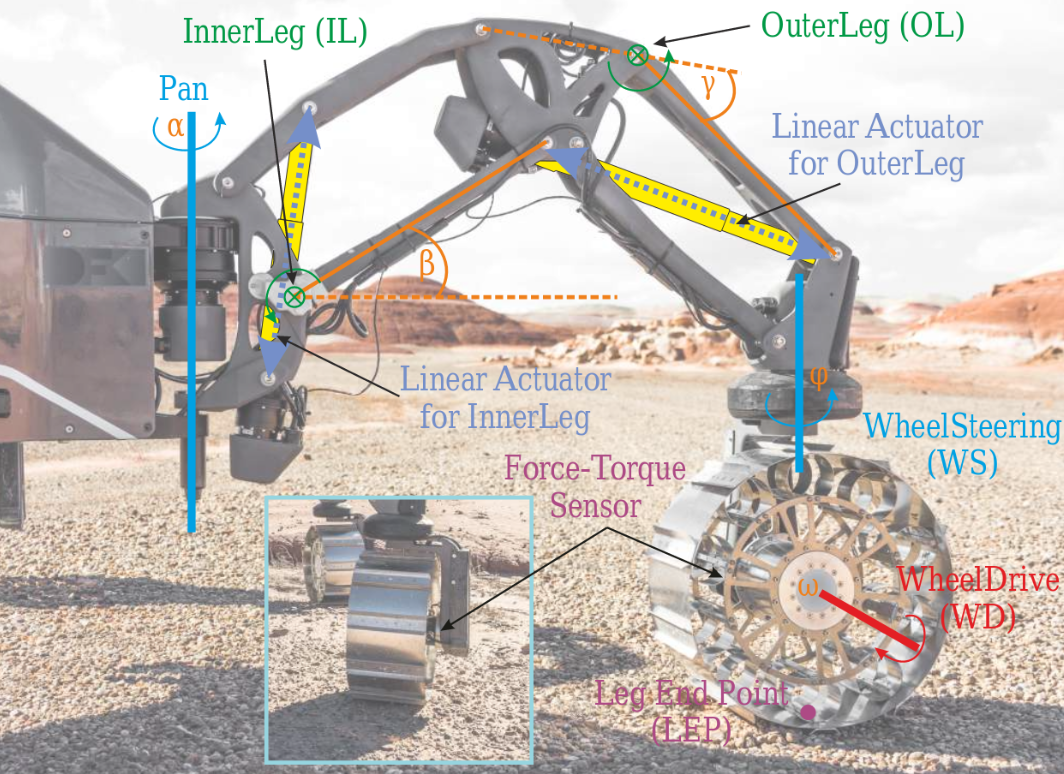
\includegraphics[width=0.6\linewidth]{sections/design/power-budget/images/sherpatt-actively-articulated-suspension-sytem.png}\\
  \caption[SherpaTT actively articulated suspension system]
          {SherpaTT actively articulated suspension system, taken from \citeother{Cordes2018}.}
  \label{fig:sherpatt-actively-articulated-suspension-system}
\end{figure}

Lack of motor optimisation as well as lower gravity and pressure on Mars permit the assumption that, given similar topology traversals, measured propulsion power draws are greater than those that would be observed on a Martian environment. This assumption is further supported when considering that SherpaTT's velocities during power draw measurements were much greater than what has been achieved on present and past Mars rover missions.

Available datasets from the Mars analogue field test campaign cover two flat surface runs and three steep upslope terrain runs. From the two upslope runs, the dataset with the worst-case maximum and mean propulsion power draw was used as the worst-case scenario. Hereafter, all mention of SherpaTT power draws will reference measurements included in these datasets. Measured power draws fluctuate due to slips, skids, noise, and other unknown imperfections. To ease readability, local minima, maxima, and media lines have been traced for all power plot figures.

\subsubsection{Flat Terrain Traverse}
\label{sec:PowerBudget:PropulsionPowerBudget:FlatTerrainTraverse}
Both \ac{MER} and \ac{MSL} rovers are each equipped with a total of 10 propulsion motors to drive their Rocker-Bogie passive suspension system: six to rotate the wheels and four to steer them \citeother{Novak2005} \citeother{Lakdawalla2018}. The \ac{MER} rovers needed approximately \SI{100}{\watt} to drive \citeother{MERRoverEnergy}. Equation \ref{eq:InitialPropulsionPowerEstimate} was used for to determine an initial SherpaTT propulsion power draw using a single \ac{MER} wheel power draw as an estimation unit:

\begin{align}
  \label{eq:InitialPropulsionPowerEstimate}
  P_{prop}^{sherpatt} &= \frac{P_{prop}^{mer}}{N_{wheels}^{mer}} \times N_{wheels}^{sherpatt} \times \left(1 +\frac{P_{susp}^{sherpatt}}{P_{prop}^{sherpatt}}\right) \\
           &= \frac{100}{6} \times 4 \times 1.17\\
           &= \SI{78}{\watt}
\end{align}


where $P_{prop}$ is the total propulsion power, $P_{susp}$ is the total suspension power, $N_{wheels}$ is the number of wheels, and $P_{susp}^{sherpatt} / P_{prop}^{sherpatt}$ is the suspension system's share of the total propulsion power. For the latter, a worst-case 17\% was taken from \citeother{Cordes2018} for data collected from a flat terrain outdoor setting.

The propulsion power draws measured for SherpaTT on flat surface runs are shown in Figure \ref{fig:plot:sherpatt-flat-terrain-power-draw}. These measurements are summarised in Table \ref{tab:sherpatt-flat-terrain-global-minimum-maximum-and-medium-power-draws}. To eliminate power draw fluctuations from the analysis, only local media values were considered. Local media were selected rather than the worst-case local maxima on the basis of the assumptions made in Section \ref{sec:PowerBudget:PropulsionPowerBudget}. For flat terrain traverses, a worst-case maximum power draw of \SI{74}{\watt} is observed in close accordance with the initial estimate obtained from Equation \ref{eq:InitialPropulsionPowerEstimate}.

\begin{figure}[h]
\captionsetup[subfigure]{justification=centering}
\vspace{-2ex}
	\centering
    %% setup sizes
    \setlength{\subfigureWidth}{0.50\textwidth}
    \setlength{\graphicsHeight}{80mm}
    %% kill hyper-link highlighting
    \hypersetup{hidelinks=true}%
    %% the figures
    \begin{subfigure}[t]{\subfigureWidth}
        \centering
        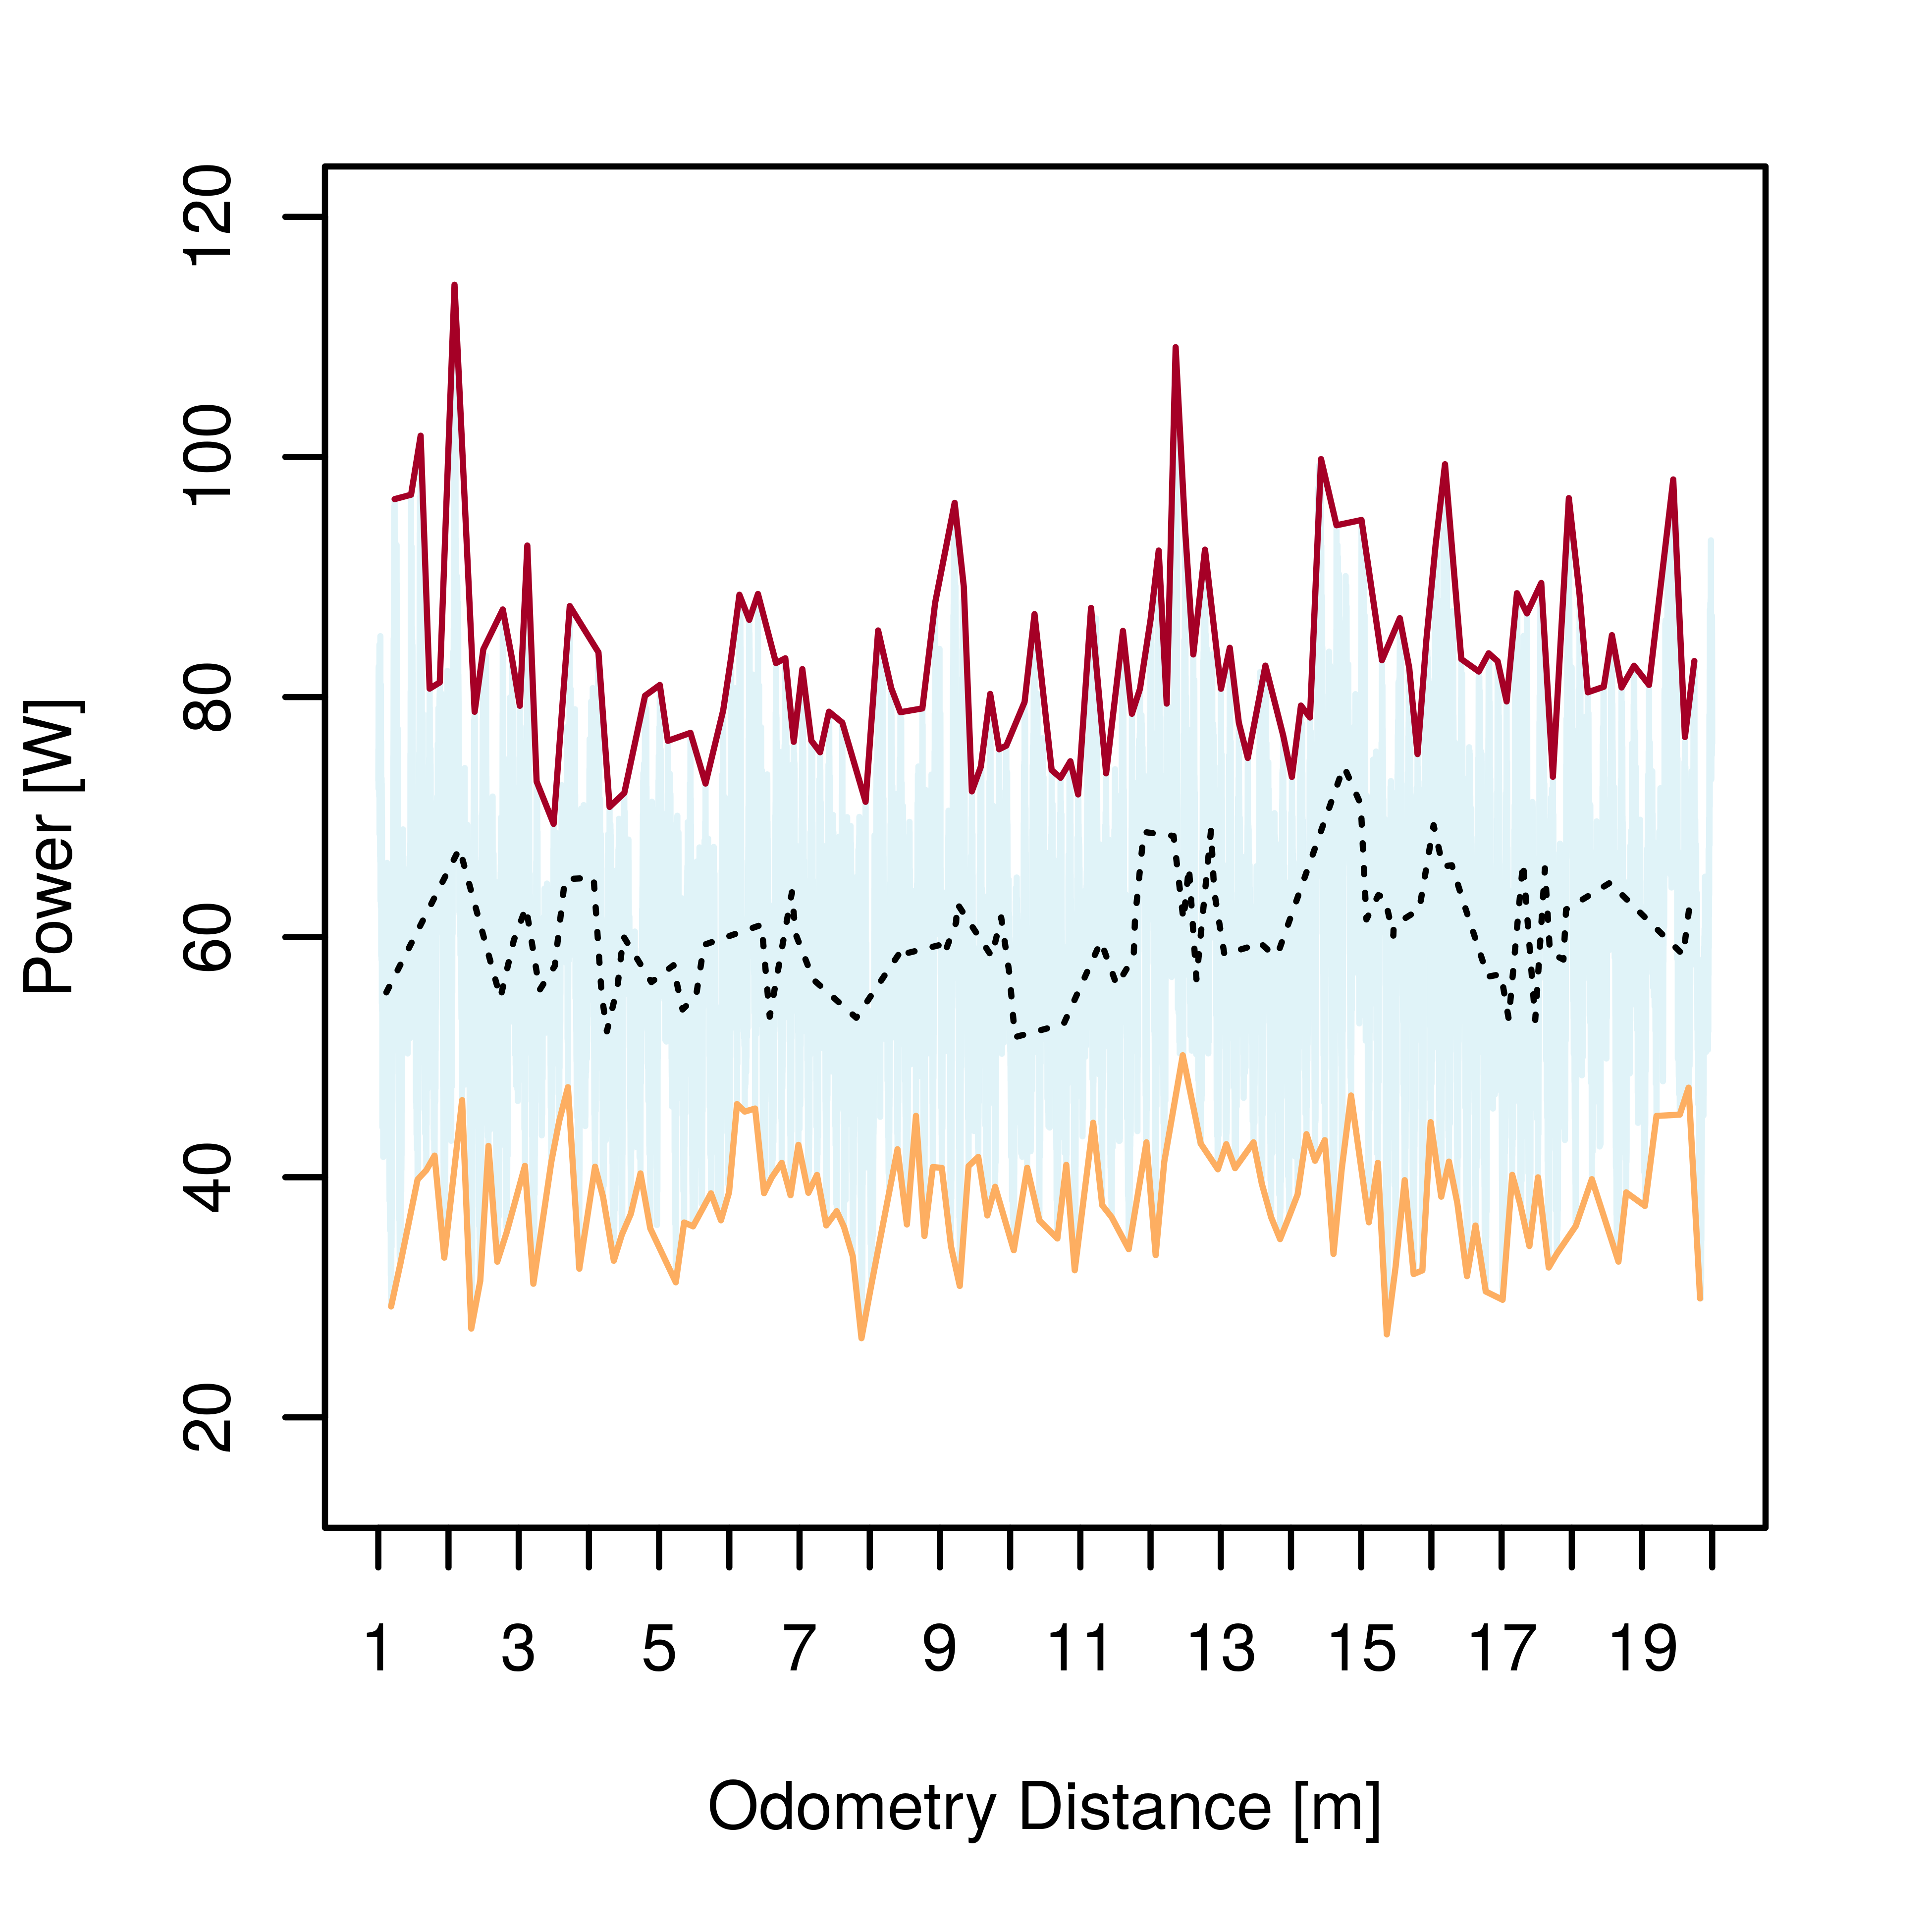
\includegraphics[height=\graphicsHeight]{sections/design/power-budget/plots/locomotion-power-draw-on-flat-terrain-1.png}
        \subcaption{Run \#1}
        \label{fig:plot:sub:sherpatt-flat-terrain-power-draw-1}
    \end{subfigure}\hfill
    \begin{subfigure}[t]{\subfigureWidth}
        \centering
        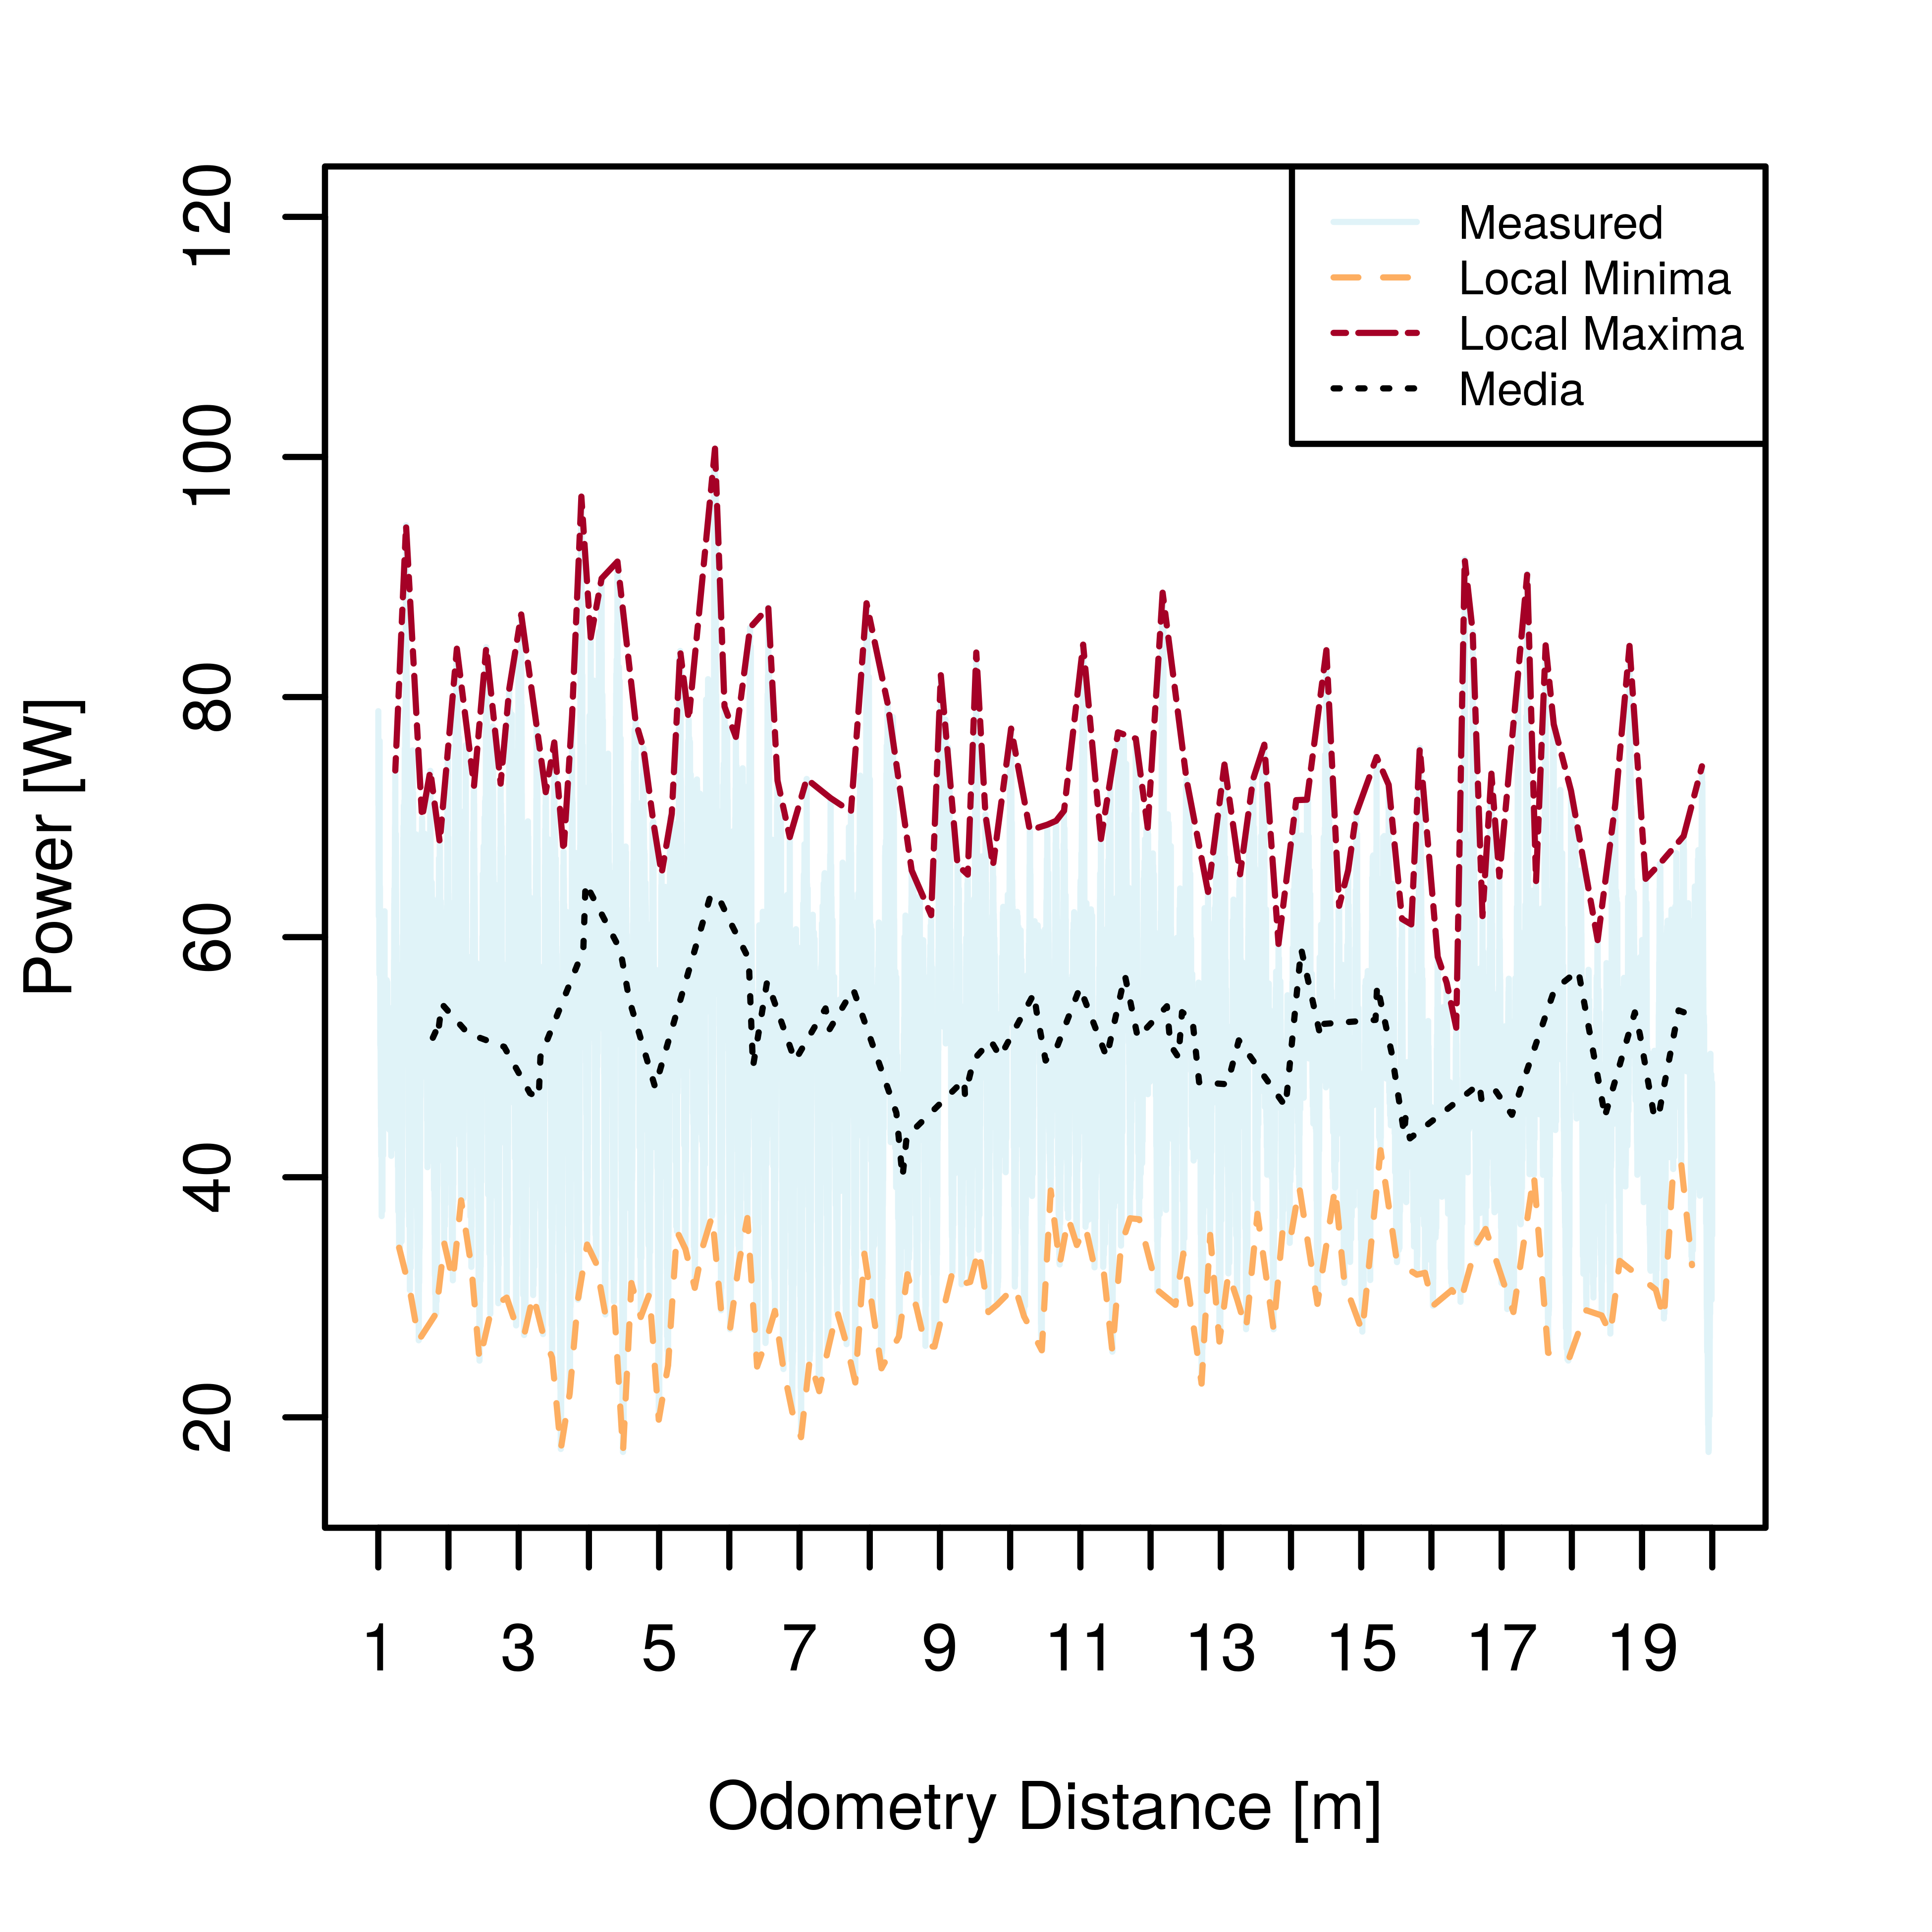
\includegraphics[height=\graphicsHeight]{sections/design/power-budget/plots/locomotion-power-draw-on-flat-terrain-2.png}
  		\subcaption{Run \#2}
		\label{fig:plot:sub:sherpatt-flat-terrain-power-draw-2}
	\end{subfigure}\\[0.8ex]
    \caption[Propulsion power draw for a flat terrain traverse during SherpaTT Mars analogue field tests in Utah]
            {Propulsion power draw for a flat terrain traverse during SherpaTT Mars analogue field tests in Utah.}
    \label{fig:plot:sherpatt-flat-terrain-power-draw}
\vspace{-2ex}
\end{figure}



\begin{table}[h]
\footnotesize
\centering
\caption[Global minimum, maximum, and medium of traced local minima, maxima, and media for SherpaTT flat terrain propulsion power draw lines]
    {Global minimum, maximum, and medium of traced local minima, maxima, and media for SherpaTT flat terrain propulsion power draw lines.}
\label{tab:sherpatt-flat-terrain-global-minimum-maximum-and-medium-power-draws}
\begin{tabular}{llccc}
\cline{3-5}
\multicolumn{2}{l|}{\multirow{2}{*}{}} & \multicolumn{3}{c|}{\textbf{Power Draw {[}W{]}}} \\ \cline{3-5}
\multicolumn{2}{l|}{} & \multicolumn{1}{c|}{\textbf{\begin{tabular}[c]{@{}c@{}}Global Minimum\end{tabular}}} & \multicolumn{1}{c|}{\textbf{\begin{tabular}[c]{@{}c@{}}Global Maximum\end{tabular}}} & \multicolumn{1}{c|}{\textbf{\begin{tabular}[c]{@{}c@{}}Global Media\end{tabular}}} \\ \hline
\multicolumn{1}{|c|}{\multirow{4}{*}{\textbf{Run \#1}}} & \multicolumn{1}{l|}{\textbf{Measured}} & \multicolumn{1}{c|}{27} & \multicolumn{1}{c|}{114} & \multicolumn{1}{c|}{60} \\ \cline{2-5}
\multicolumn{1}{|c|}{} & \multicolumn{1}{l|}{\textbf{Local Minima}} & \multicolumn{1}{c|}{27} & \multicolumn{1}{c|}{50} & \multicolumn{1}{c|}{38} \\ \cline{2-5}
\multicolumn{1}{|c|}{} & \multicolumn{1}{l|}{\textbf{Local Maxima}} & \multicolumn{1}{c|}{69} & \multicolumn{1}{c|}{114} & \multicolumn{1}{c|}{83} \\ \cline{2-5}
\multicolumn{1}{|c|}{} & \multicolumn{1}{l|}{\textbf{Local Media}} & \multicolumn{1}{c|}{52} & \multicolumn{1}{c|}{74} & \multicolumn{1}{c|}{61} \\ \hhline{|=|=|=|=|=|}
\multicolumn{1}{|l|}{\multirow{4}{*}{\textbf{Run \#2}}} & \multicolumn{1}{l|}{\textbf{Measured}} & \multicolumn{1}{c|}{17} & \multicolumn{1}{c|}{101} & \multicolumn{1}{c|}{51} \\ \cline{2-5}
\multicolumn{1}{|l|}{} & \multicolumn{1}{l|}{\textbf{Local Minima}} & \multicolumn{1}{c|}{17} & \multicolumn{1}{c|}{42} & \multicolumn{1}{c|}{30} \\ \cline{2-5}
\multicolumn{1}{|l|}{} & \multicolumn{1}{l|}{\textbf{Local Maxima}} & \multicolumn{1}{c|}{52} & \multicolumn{1}{c|}{101} & \multicolumn{1}{c|}{74} \\ \cline{2-5}
\multicolumn{1}{|l|}{} & \multicolumn{1}{l|}{\textbf{Local Media}} & \multicolumn{1}{c|}{40} & \multicolumn{1}{c|}{64} & \multicolumn{1}{c|}{52} \\ \hline
 &  & \multicolumn{1}{l}{} & \multicolumn{1}{l}{} & \multicolumn{1}{l}{} \\
 &  & \multicolumn{1}{l}{} & \multicolumn{1}{l}{} & \multicolumn{1}{l}{}
\end{tabular}
\end{table}


\pagebreak
\subsubsection{Upslope Terrain Traverse}
\label{sec:PowerBudget:PropulsionPowerBudget:UpslopeTerrainTraverse}
Propulsion power draws on a steep uplsope were measured along an approximately \SI{16}{\meter} track and are shown Figure \ref{fig:plot:sub:sherpatt-disaggregated-upslope-terrain-power-draw-locomotion}. An initial estimate of \SI{132}{\watt} was obtained using Equation \ref{eq:InitialPropulsionPowerEstimate} with a worst case 98\% suspension system's share of the total propulsion power taken from \citeother{Cordes2018} for data collected from a steep slope outdoor setting. The drive and suspension power draw components are shown in Figures \ref{fig:plot:sub:sherpatt-disaggregated-upslope-terrain-power-draw-drive} and \ref{fig:plot:sub:sherpatt-disaggregated-upslope-terrain-power-draw-suspension}, respectively.

\begin{figure}[h]
\captionsetup[subfigure]{justification=centering}
\vspace{-2ex}
	\centering
    %% setup sizes
    \setlength{\subfigureWidth}{0.32\textwidth}
    \setlength{\graphicsHeight}{50mm}
    %% kill hyper-link highlighting
    \hypersetup{hidelinks=true}%
    %% the figures
	\begin{subfigure}[t]{\subfigureWidth}
        \centering
        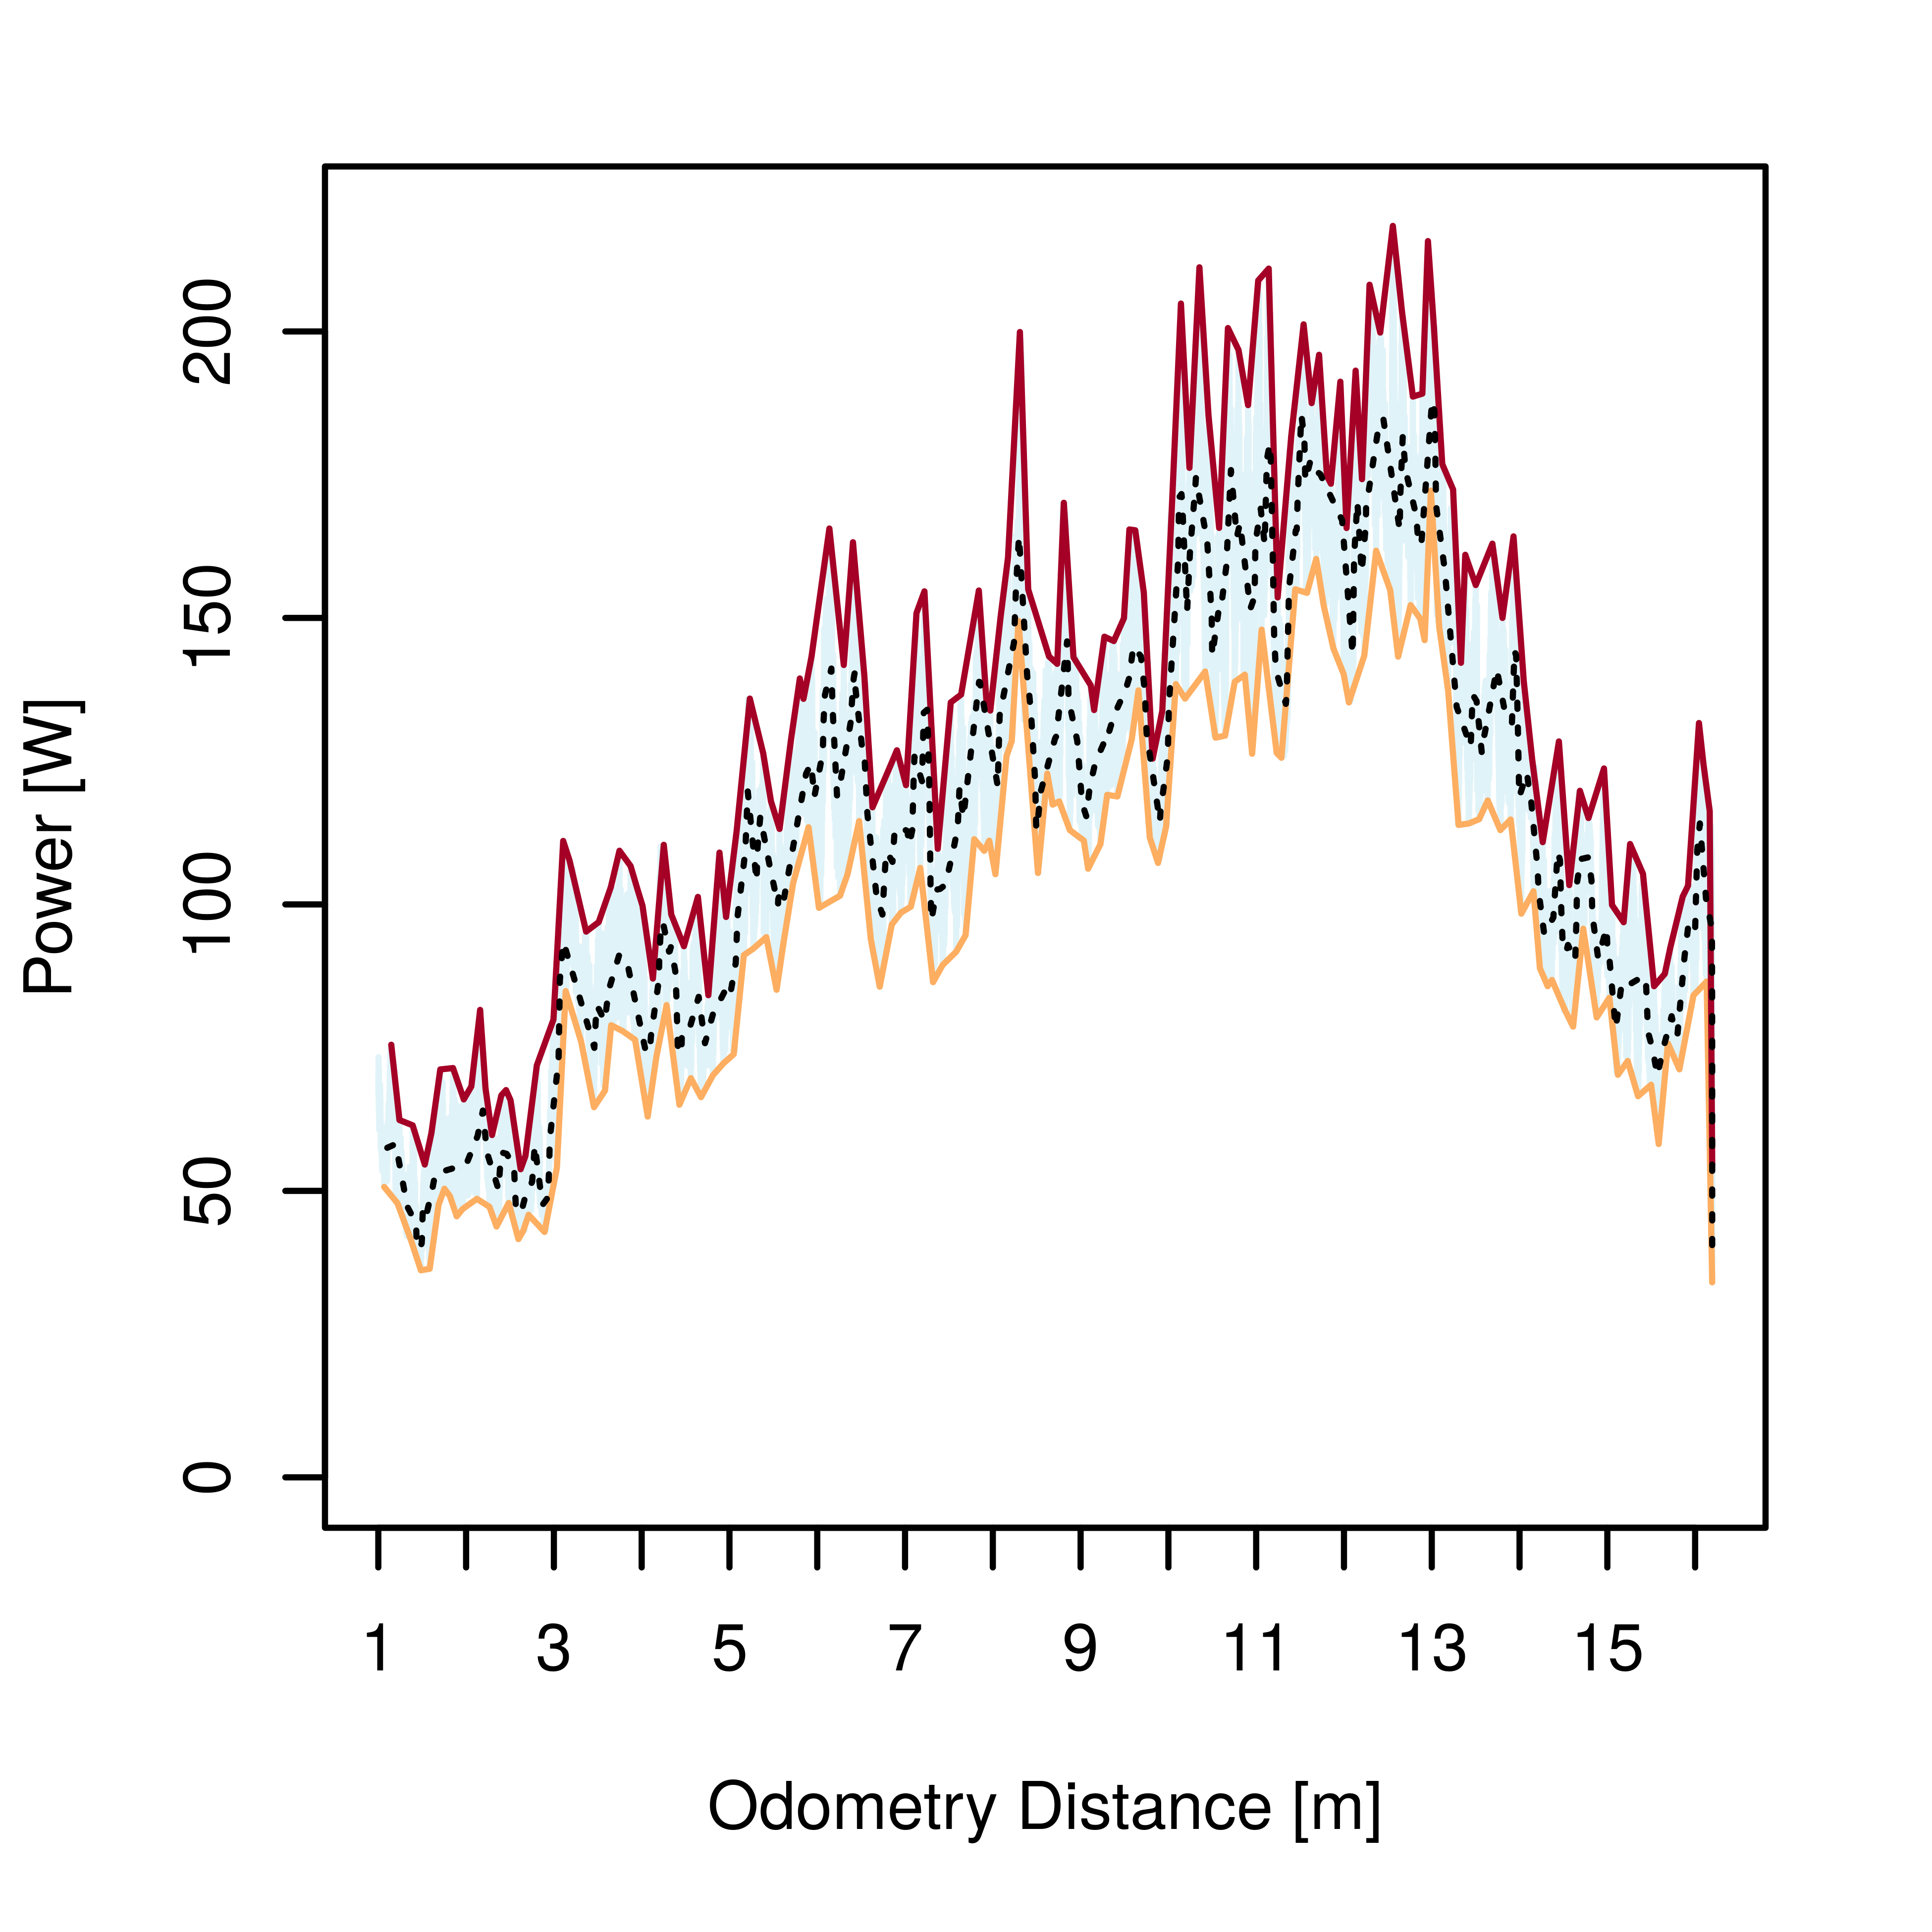
\includegraphics[height=\graphicsHeight]{sections/design/power-budget/plots/locomotion-power-draw-on-upslope-terrain.png}
  		\subcaption{Propulsion}
		\label{fig:plot:sub:sherpatt-disaggregated-upslope-terrain-power-draw-locomotion}
	\end{subfigure}\hfill
	\begin{subfigure}[t]{\subfigureWidth}
        \centering
        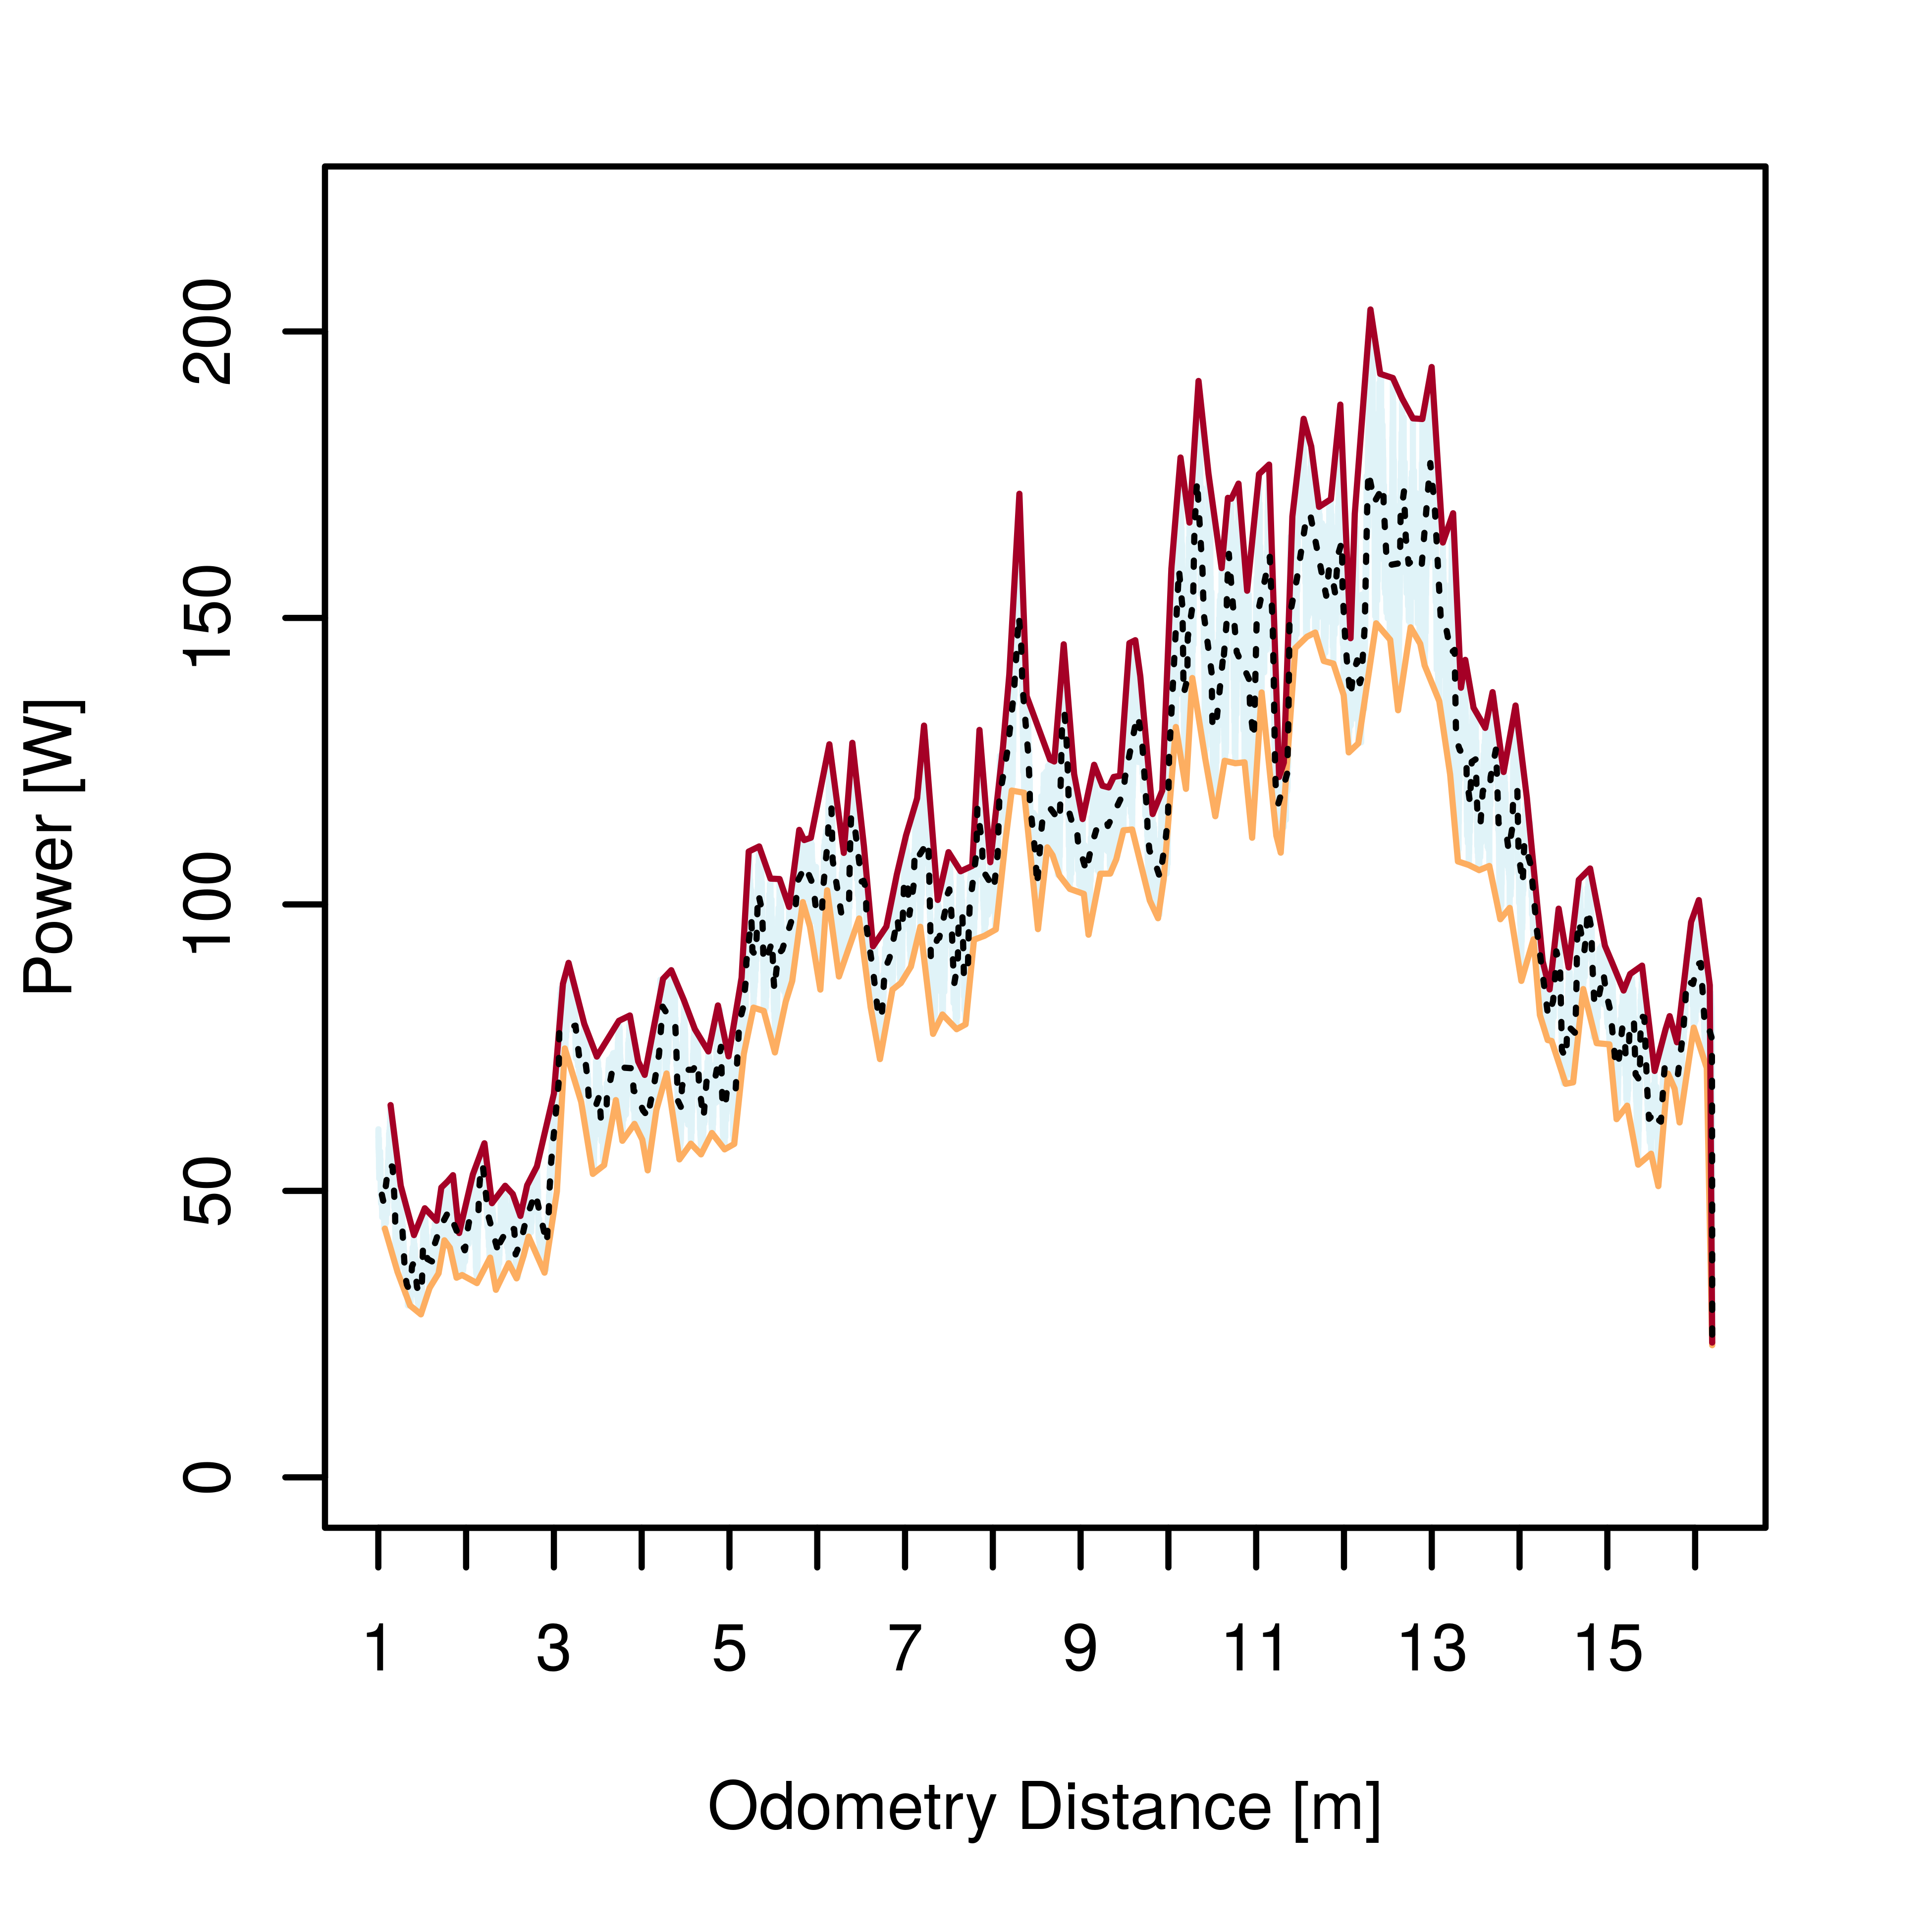
\includegraphics[height=\graphicsHeight]{sections/design/power-budget/plots/drive-power-draw-on-upslope-terrain.png}
  		\subcaption{Drive}
		\label{fig:plot:sub:sherpatt-disaggregated-upslope-terrain-power-draw-drive}
	\end{subfigure}\hfill
    \begin{subfigure}[t]{\subfigureWidth}
        \centering
        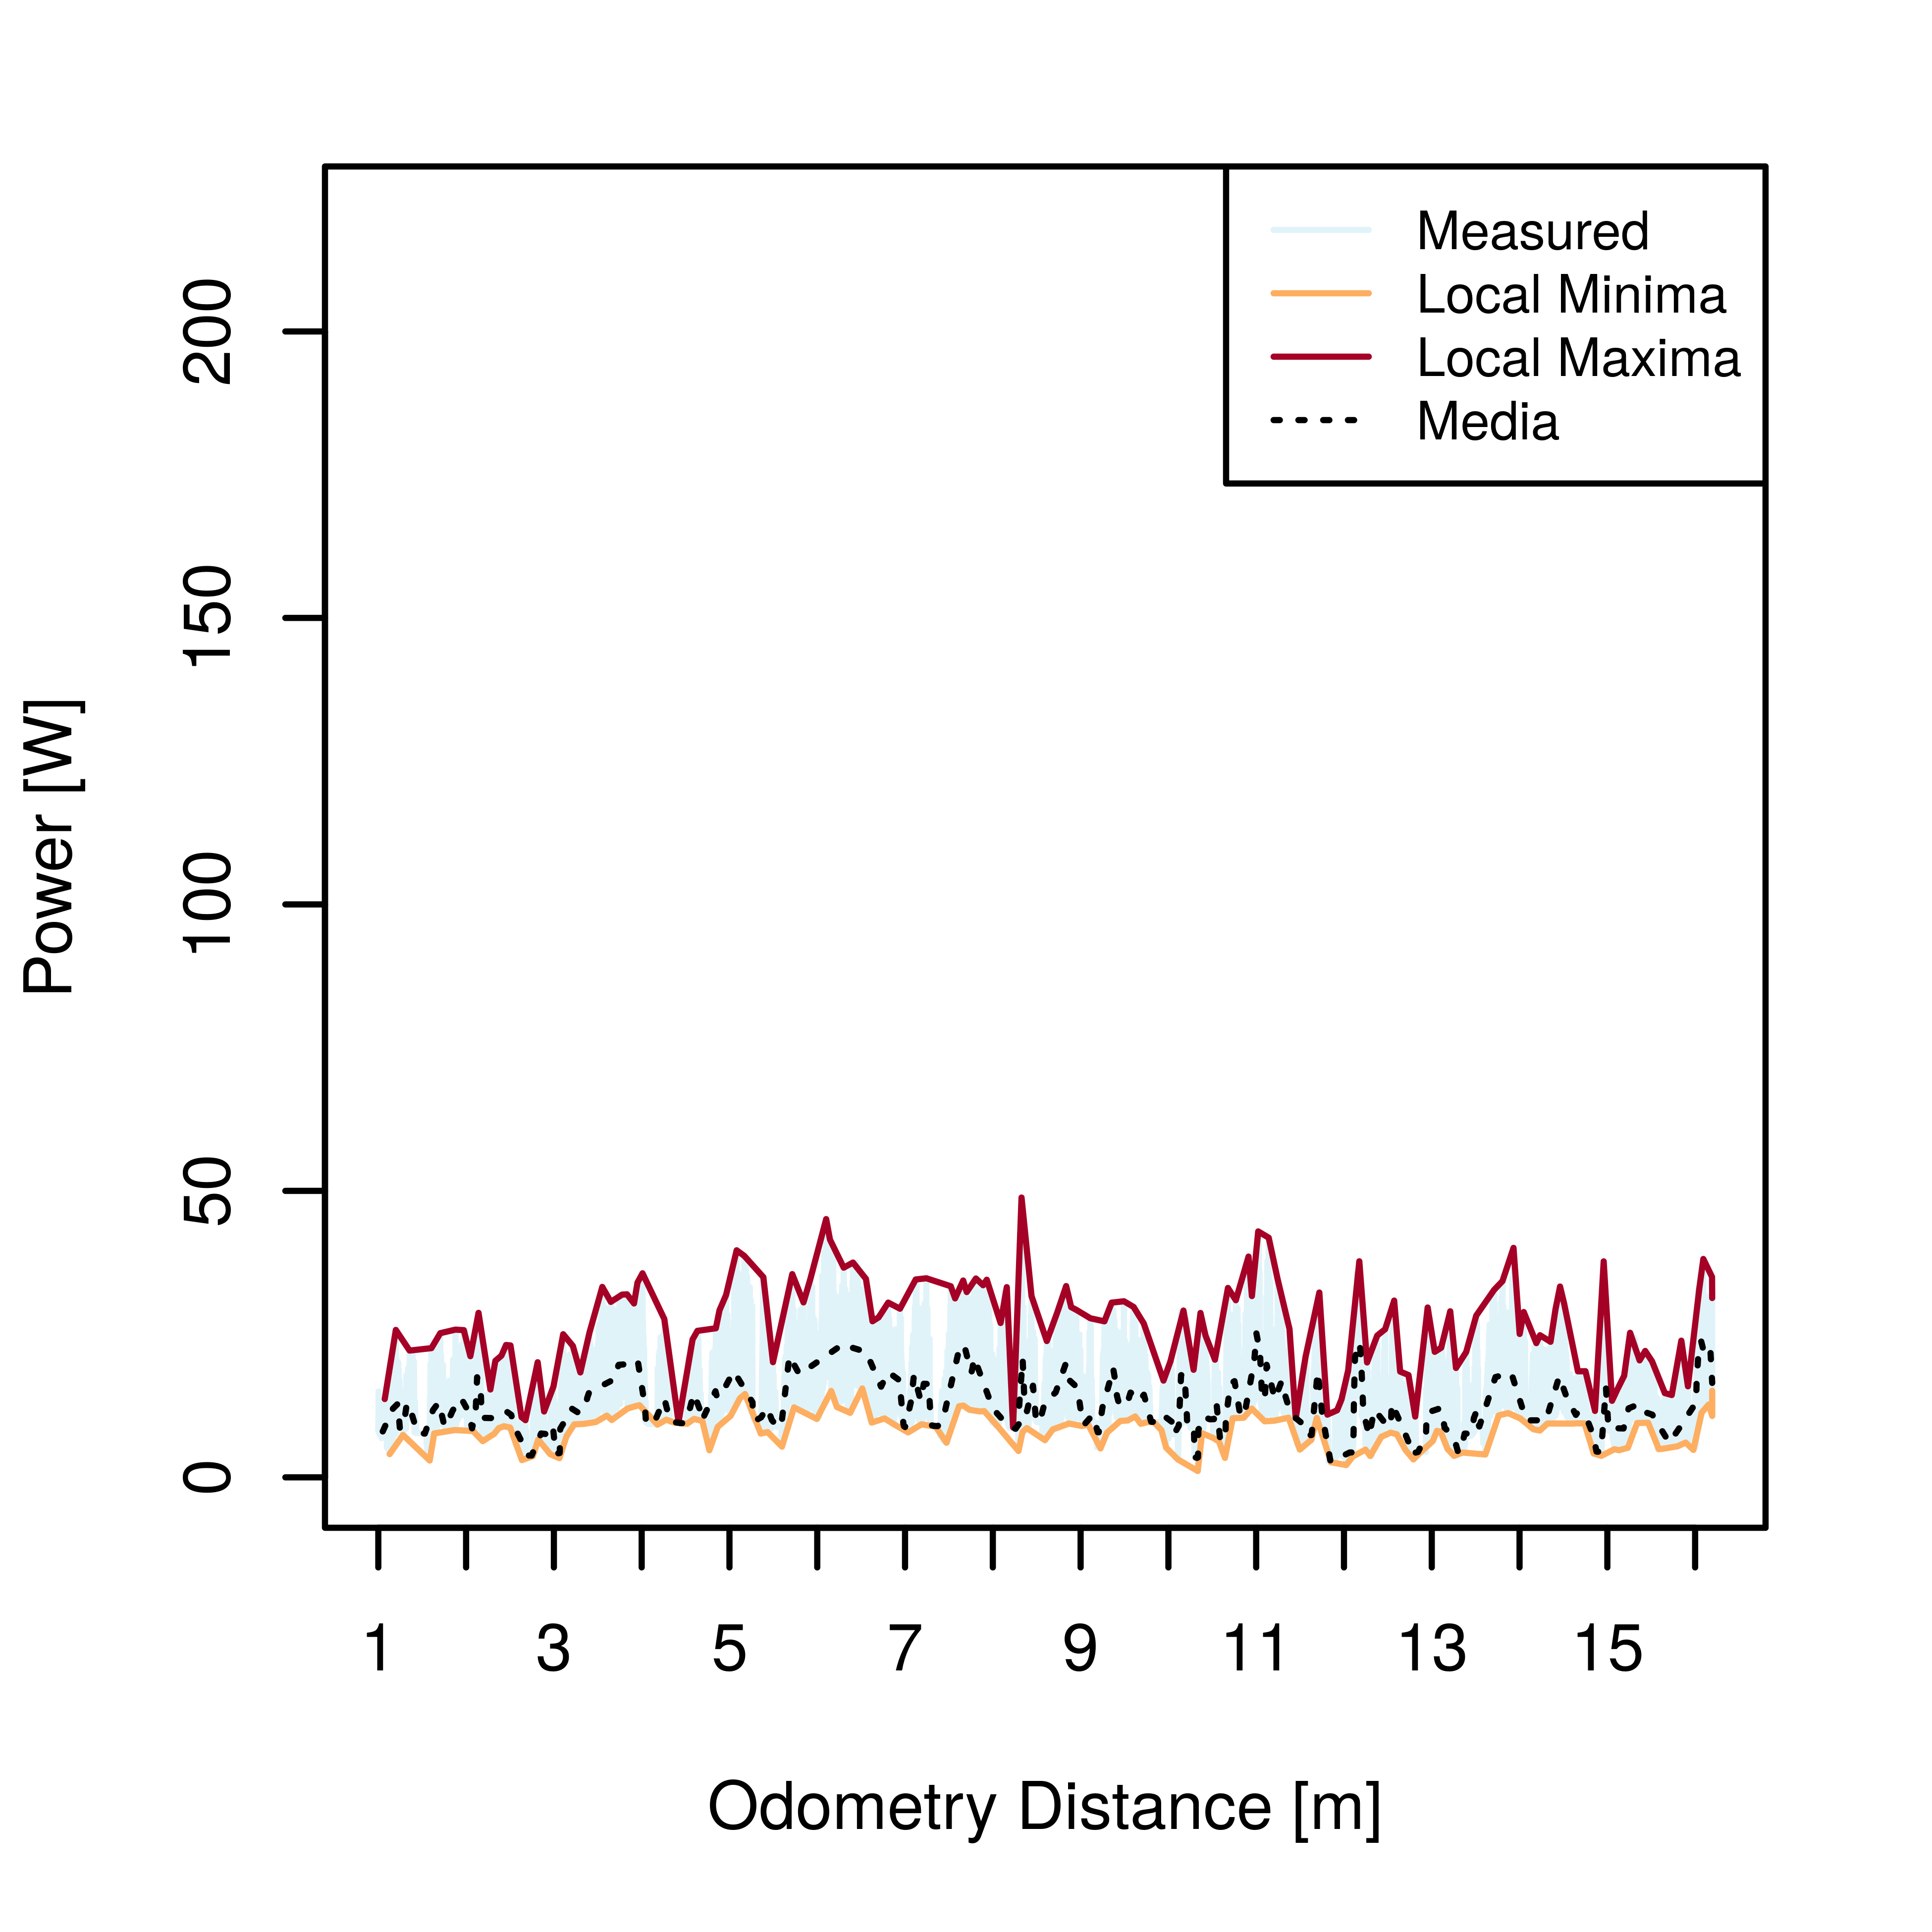
\includegraphics[height=\graphicsHeight]{sections/design/power-budget/plots/suspension-power-draw-on-upslope-terrain.png}
  		\subcaption{Suspension}
		\label{fig:plot:sub:sherpatt-disaggregated-upslope-terrain-power-draw-suspension}
	\end{subfigure}\\[0.8ex]
    \caption[Disaggregated measurements of power draw for upslope terrain traverse during SherpaTT Mars analogue field tests in Utah]
            {Disaggregated measurements of power draw for upslope terrain traverse during SherpaTT Mars analogue field tests in Utah.}
    \label{fig:plot:sherpatt-disaggregated-upslope-terrain-power-draw}
\vspace{-2ex}
\end{figure}

An uplsope traverse has no discernable effect on the suspension power draw, however; there is a clear gradual increase in the drive power draw. The global maximum, minimum, and medium of the traced local minima, maxima, and media power draw lines are presented in Table \ref{tab:sherpatt-upslope-terrain-global-minimum-maximum-and-medium-power-draws}.

\begin{table}[h]
\footnotesize
\centering
\caption[Global minimum, maximum, and medium of traced local minima, maxima, and media for SherpaTT upslope terrain traverse propulsion power draw lines]
    {Global minimum, maximum, and medium of traced local minima, maxima, and media for SherpaTT upslope terrain traverse propulsion power draw lines.}
\label{tab:sherpatt-upslope-terrain-global-minimum-maximum-and-medium-power-draws}
\begin{tabular}{l|c|c|c|}
\cline{2-4}
\multicolumn{1}{c|}{\multirow{2}{*}{\textbf{}}} & \multicolumn{3}{c|}{\textbf{Power Draw {[}W{]}}} \\ \cline{2-4}
\multicolumn{1}{c|}{} & \textbf{\begin{tabular}[c]{@{}c@{}}Global Minimum\end{tabular}} & \textbf{\begin{tabular}[c]{@{}c@{}}Global Maximum\end{tabular}} & \textbf{\begin{tabular}[c]{@{}c@{}}Global Media\end{tabular}} \\ \hline
\multicolumn{1}{|l|}{\textbf{Measured}} & 34 & 218 & 114 \\ \hline
\multicolumn{1}{|l|}{\textbf{Local Minima}} & 34 & 172 & 98 \\ \hline
\multicolumn{1}{|l|}{\textbf{Local Maxima}} & 54 & 218 & 133 \\ \hline
\multicolumn{1}{|l|}{\textbf{Local Media}} & 40 & 188 & 18 \\ \hline
\end{tabular}
\end{table}


\pagebreak
Figure \ref{fig:plot:sherpatt-upslope-terrain-power-draw} overlaps the propulsion local media power draws with the tackled slope angles. The steepest slope angle was \SI{28}{\degree} for an average of \SI{17.52}{\degree}. Slope angle increase are consistently followed by power draw spikes, i.e. at approximately 3, 4, 5, 6, 8, and 9 \si{\meter} in the odometry measurements. Inversely, slope angle decreases were followed by power draws troughs at approximately 11, 13, 14, and 16 \si{\meter}.

\begin{figure}[h]
  \centering
  \hypersetup{linkcolor=captionTextColor}
  \includegraphics[width=0.8\linewidth]{sections/design/power-budget/plots/minima-locomotion-power-draws-on-upslope-terrain.png}\\
  \caption[Mean Propulsion power draw for an upslope terrain traverse during SherpaTT Utah field test campaign.]
          {Mean Propulsion power draw for an upslope terrain traverse during SherpaTT Utah field test campaign.}
  \label{fig:plot:sherpatt-upslope-terrain-power-draw}
\end{figure}


The power draws trough following the slope angle change from \SI{28}{\degree} to \SI{20}{\degree} at the \SI{11}{\meter} mark is subsequently followed by an unusual power draw increase and fluctuation. These measurements were discarded as they are outliers with respect to the power draw responses for the slope angle descreases that followed.

Table \ref{tab:sherpatt-upslope-terrain-local-media-measurement-summary} summarises the minimum, maximum, and mean local media propulsion power draws that were measured for different slope angles. Discarding the outlier measurements subsequent to the slope angle change from \SI{28}{\degree} to \SI{20}{\degree} at the \SI{11}{\meter} to \SI{13}{\meter} portion of the track, the maximum mean local media propulsion power draw is \SI{146}{\watt}, which is close to the initial estimate given by Equation \ref{eq:InitialPropulsionPowerEstimate}.

\begin{table}[h]
\footnotesize
\centering
\caption[SherpaTT mean propulsion power draw measurements for different slope sections]
    {SherpaTT mean propulsion power draw measurements for different slope sections.}
\label{tab:sherpatt-upslope-terrain-local-media-measurement-summary}
\begin{tabular}{cc|c|c|c|}
\cline{3-5}
\multicolumn{1}{l}{} & \multicolumn{1}{l|}{} & \multicolumn{3}{c|}{\textbf{Power {[}W{]}}} \\ \hline
\multicolumn{1}{|l|}{\textbf{Distance {[}m{]}}} & \multicolumn{1}{l|}{\textbf{Slope Angle {[}deg{]}}} & \multicolumn{1}{l|}{\textbf{Minimum}} & \multicolumn{1}{l|}{\textbf{Maximum}} & \multicolumn{1}{l|}{\textbf{Mean}} \\ \hline
\multicolumn{1}{|c|}{\textbf{1 $<$ x $\leq$ 3}} & 10 & 40 & 64 & 51 \\ \hline
\multicolumn{1}{|c|}{\textbf{3 $<$ x $\leq$ 4}} & 11 & 73 & 93 & 85 \\ \hline
\multicolumn{1}{|c|}{\textbf{4 $<$ x $\leq$ 5}} & 15 & 74 & 87 & 83 \\ \hline
\multicolumn{1}{|c|}{\textbf{5 $<$ x $\leq$ 6}} & 16 & 85 & 125 & 107 \\ \hline
\multicolumn{1}{|c|}{\textbf{6 $<$ x $\leq$ 7}} & 28 & 98 & 141 & 123 \\ \hline
\multicolumn{1}{|c|}{\textbf{7 $<$ x $\leq$ 8}} & 22 & 97 & 139 & 116 \\ \hline
\multicolumn{1}{|c|}{\textbf{8 $<$ x $\leq$ 9}} & 25 & 113 & 164 & 133 \\ \hline
\multicolumn{1}{|c|}{\textbf{9 $<$ x $\leq$ 11}} & 28 & 114 & 176 & 146 \\ \hline
\multicolumn{1}{|c|}{\textbf{11 $<$ x $\leq$ 13}} & 20 & 135 & 188 & 167 \\ \hline
\multicolumn{1}{|c|}{\textbf{13 $<$ x $\leq$ 14}} & 15 & 119 & 123 & 145 \\ \hline
\multicolumn{1}{|c|}{\textbf{14 $<$ x $\leq$ 16}} & 10 & 70 & 186 & 94 \\ \hline
\end{tabular}
\end{table}


\pagebreak
\subsection{Traverse Power Budget}
\label{sec:PowerBudget:PowerBudget:TraversePowerBudget}
Worst-case daily insolations for an optical depth of $\tau = 1$ were used to determine the energy requirements of the flat and upslope traverse reference Sols and were taken from Tables \ref{tab:insolation-iani-chaos-clear-and-dusty-days} for Iani Chaos and \ref{tab:insolation-ismenius-cavus-clear-and-dusty-days} for Ismenius Cavus. The minimum required traverse distance was assumed to be \SI{5}{\meter} at both mission sites.

\subsubsection{Flat Traverse}
\label{sec:Design:PowerBudget:TraversePowerBudget:FlatTraverse}

Power and duration of \textit{DTE Communication}, \textit{Science Stop - Short}, and \textit{Hibernation} modes were taken from \citeother{CDF2014} and assigned to the reference Sols presented in Section \ref{sec:ReferenceSols:ReferenceSols}. Power draw estimates made in Sections \ref{sec:PowerBudget:PropulsionPowerBudget:FlatTerrainTraverse} and \ref{sec:PowerBudget:PropulsionPowerBudget:UpslopeTerrainTraverse} were used for \textit{Traverse} modes. Power draw for the \textit{Optimal Pose} mode was equated to that of the rover's flat terrain propulsion power and etimated to take up to \SI{10}{\minute}. The worst-case power budget for the reference \textit{Flat Traverse Sol} is shown in Table \ref{tab:worst-case-traverse-sol-power-budget}.

\begin{table}[h]
\footnotesize
\centering
\caption[Worst-case mission site flat terrain traverse Sol power budget]
    {Worst-case mission site flat terrain traverse Sol power budget for $\tau=1$.}
\label{tab:worst-case-traverse-sol-power-budget}
\begin{tabular}{lc|c|c|c|c|}
\cline{3-6}
 & \textbf{} & \multicolumn{2}{c|}{\textbf{\begin{tabular}[c]{@{}c@{}}Iani Chaos\\ $Ls=\SI{81}{\degree}$\end{tabular}}} & \multicolumn{2}{c|}{\textbf{\begin{tabular}[c]{@{}c@{}}Ismenius Cavus\\ $Ls=\SI{273}{\degree}$\end{tabular}}} \\ \hline
\multicolumn{1}{|l|}{\textbf{Mode}} & \textbf{P {[}W{]}} & \textbf{t {[}min{]}} & \textbf{E {[}Wh{]}} & \textbf{t {[}min{]}} & \textbf{E {[}Wh{]}} \\ \hline
\multicolumn{1}{|l|}{\textbf{Idle - Day}} & 29 & 603 & 291 & 464 & 224 \\ \hline
\multicolumn{1}{|l|}{\textbf{DTE Communication}} & 52 & 35 & 30 & 35 & 30 \\ \hline
\multicolumn{1}{|l|}{\textbf{Traverse - Flat}} & 113\footnote{Power draws taken from \citeother{CDF2014} for Communications, \ac{DHS}, \ac{GNC}, and \ac{PCDU} are added to the \SI{75}{\watt} flat terrain propulsion power draw resulting in a total \textit{Traverse Mode} power budget of \SI{113}{\watt}.} & 4.8 & 9 & 4.8 & 9 \\ \hline
\multicolumn{1}{|l|}{\textbf{Science Stop - Short}} & 60 & 60 & 60 & 60 & 60 \\ \hline
\multicolumn{1}{|l|}{\textbf{Optimal Pose}} & 75 & 12 & 13 & 10 & 13 \\ \hline
\multicolumn{1}{|l|}{\textbf{Idle - Night}} & 20 & 242 & 242 & 866 & 289 \\ \hline
\multicolumn{1}{|r|}{\textbf{Total}} & \textbf{349} & \textbf{1440} & \textbf{646} & \textbf{1440} & \textbf{625} \\ \hline
\multicolumn{1}{|r|}{\textbf{Total +20\% System Margin}} & \textbf{419} & - & \textbf{775} & - & \textbf{750} \\ \hline
\end{tabular}
\end{table}


The total energy requirements for these worst-case reference Sols were used as the minimum energy output when sizing the \ac{SA}. A 20\% system margin was applied to account for unaccounted inefficiencies such as \ac{PCDU} losses.

\subsubsection{Upslope Traverse}
\label{sec:Design:PowerBudget:TraversePowerBudget:UpslopeTraverse}
The worst-case upslope traverese reference Sols shown in Table \ref{tab:worst-case-upslope-traverse-sol-power-budget} only differ from their flat traverse equivalents by the \textit{Traverse} mode power draw. It is increased from \SI{75}{\watt} to \SI{150}{\watt}.

\begin{table}[h]
\footnotesize
\centering
\caption[Worst-case upslope traverse Sol power budget at mission sites]
    {Worst-case upslope traverse Sol power budget at mission sites for $\tau =1$.}
\label{tab:worst-case-upslope-traverse-sol-power-budget}
\begin{tabular}{lc|c|c|c|c|}
\cline{3-6}
 & \textbf{} & \multicolumn{2}{c|}{\textbf{\begin{tabular}[c]{@{}c@{}}Iani Chaos\\ $Ls=\SI{81}{\degree}$\end{tabular}}} & \multicolumn{2}{c|}{\textbf{\begin{tabular}[c]{@{}c@{}}Ismenius Cavus\\ $Ls=\SI{273}{\degree}$\end{tabular}}} \\ \hline
\multicolumn{1}{|l|}{\textbf{Mode}} & \textbf{P {[}W{]}} & \textbf{t {[}min{]}} & \textbf{E {[}Wh{]}} & \textbf{t {[}min{]}} & \textbf{E {[}Wh{]}} \\ \hline
\multicolumn{1}{|l|}{\textbf{Idle - Day}} & 29 & 603 & 291 & 464 & 224 \\ \hline
\multicolumn{1}{|l|}{\textbf{DTE Communication}} & 52 & 35 & 30 & 35 & 30 \\ \hline
\multicolumn{1}{|l|}{\textbf{Traverse - Upslope}} & 188\footnote{Power draws taken from \citeother{CDF2014} for Communications, \ac{DHS}, \ac{GNC}, and \ac{PCDU} are added to the \SI{150}{\watt} flat terrain propulsion power draw resulting in a total \textit{Traverse Mode} power budget of \SI{188}{\watt}.} & 4.8 & 9 & 4.8 & 15 \\ \hline
\multicolumn{1}{|l|}{\textbf{Science Stop - Short}} & 60 & 60 & 60 & 60 & 60 \\ \hline
\multicolumn{1}{|l|}{\textbf{Optimal Pose}} & 75 & 12 & 13 & 10 & 13 \\ \hline
\multicolumn{1}{|l|}{\textbf{Idle - Night}} & 20 & 242 & 242 & 866 & 289 \\ \hline
\multicolumn{1}{|r|}{\textbf{Total}} & \textbf{424} & \textbf{1440} & \textbf{652} & \textbf{1440} & \textbf{631} \\ \hline
\multicolumn{1}{|r|}{\textbf{Total +20\% System Margin}} & \textbf{509} & - & \textbf{782} & - & \textbf{757} \\ \hline
\end{tabular}
\end{table}


These worst-case reference Sols were not considered in \ac{SA} sizing. Regardless, they are presented for the sake of comparative analysis with the flat traverse equivalent.


\subsubsection{Hibernation}
\label{sec:Design:PowerBudget:TraversePowerBudget:Hibernation}
The power budget for the reference \textit{Hibernation Sol} is shown in Table \ref{tab:hibernation-sol-power-budget}. The \SI{18}{\watt} power draw was taken from \citeother{CDF2014}.

\begin{table}[h]
\footnotesize
\centering
\caption[Hibernation Sol power budget]
    {Hibernation Sol power budget.}
\label{tab:hibernation-sol-power-budget}
\begin{tabular}{lc|c|c|c|c|}
\cline{3-6}
 & \textbf{} & \multicolumn{2}{c|}{\textbf{Iani Chaos}} & \multicolumn{2}{c|}{\textbf{Ismenius Cavus}} \\ \hline
\multicolumn{1}{|l|}{\textbf{Mode}} & \textbf{P {[}W{]}} & \textbf{t {[}min{]}} & \textbf{E {[}Wh{]}} & \textbf{t {[}min{]}} & \textbf{E {[}Wh{]}} \\ \hline
\multicolumn{1}{|l|}{\textbf{Hibernation - Day}} & 18 & 720 & 216 & 720 & 216 \\ \hline
\multicolumn{1}{|l|}{\textbf{Hibernation - Night}} & 18 & 720 & 216 & 720 & 216 \\ \hline
\multicolumn{1}{|r|}{\textbf{Total}} & \textbf{36} & \textbf{1440} & \textbf{432} & \textbf{1440} & \textbf{432} \\ \hline
\multicolumn{1}{|r|}{\textbf{Total +20\% System Margin}} & \textbf{43} & - & \textbf{518} & - & \textbf{518} \\ \hline
\end{tabular}
\end{table}


\subsection{Summary}
\label{sec:PowerBudget:Summary}
\todo[inline]{\textbf{TODO:} Write section summary.}


\clearpage
\section{Requirements and Design Drivers}
\label{sec:Design:RequirementsAndDesignDrivers}
Requirements and design drivers constrain the rover's \ac{SA} design. This section reviews and complements the assumptions made thus far. The selected solar cell technology and the assumptions pertaining to its \ac{BOL} and \ac{EOL} efficiencies are also presented. Further assumptions are made regarding the rover's mobility capabilities.


\subsection{Assumptions}
\label{sec:RequirementsAndDesignDrivers:Assumptions}
The assumptions are:

\begin{enumerate}[label=\textbf{\textcolor{BulletBlue}{A-\arabic*}}]
    \item Propulsion power draw for flat terrain traverses is \SI{75}{\watt}.
    \item Propulsion power draw for upslope terrain traverses up to \SI{30}{\degree} inclination is \SI{150}{\watt}.
    \item Solar cell technology is \ac{IMM} solar cell with AM0 efficiency of 32.3\% at \ac{BOL} and 22.5\% at \ac{EOL} \citepower{Sharps2017}.
    \item \label{itm:ass:solar_cell_efficiency} \ac{IMM} Solar cell efficiency on Mars surface is 22\% at \ac{EOL}.
    \item \label{itm:ass:packing_efficiency} Solar cell packing efficiency is 85\%.
    \item \label{itm:ass:red_shifts} Solar array efficiency varies by 3\% due to changing temperature and red-shift spectral losses through the day time-period \citepower{Kerslake1999}.
    \item \label{itm:ass:dust_deposition_saturation} Solar array dust performance degradation saturates at 30\% \citepower{Stella2005}.
    \item \label{itm:ass:protruding_shadowing} Solar array performance degradation from shadowing by protruding rover structures is 5\%.
    \item \label{itm:ass:sa_surface_density} The \ac{SA} surface density is \SI{3.7}{kg.m^{-2}}.
    \item The rover's nominal velocity is at least \SI{2}{cm.s^{-2}}.
    \item There is an average 15\% slippage when traversing a flat terrains for any given distance \citeother{Cordes2018}.
    \item There is an average 30\% slippage when traversing an upslope terrain for any given distance and slope angle \citeother{Cordes2018}.
\end{enumerate}

\subsection{Requirements}
\label{sec:sec:Design:RequirementsAndDesignDrivers:Requirements}
The following considerations are taken into account to narrow down the requirements:

\begin{enumerate}[label=\textbf{\textcolor{BulletBlue}{(\alph*)}}]
    \item Interest in long traverses from the PERASPERA programme on space robotics \citeother{PERASPERA}.
    \item Focus on space robotics development for long autonomous traverses at \ac{DFKI} \citeother{OG6} \citeother{OG10}.
    \item Mission site at Iani Chaos is approximately \SI{100}{\kilo\meter} from closest resource deposits of interest.
    \item Area of interest at Ismenius Cavus is approximately $\SI{100}{\kilo\meter} \times \SI{50}{\kilo\meter}$.
    \item Dust storm tracking in \citemarsenv{Battalio2019} observed that the average duration of local dust storms is approximately seven Sols.
\end{enumerate}

The following \ac{EOL} requirements apply for a mission life time of one \ac{MY}:

\begin{enumerate}[label=\textbf{\textcolor{BulletBlue}{R-\arabic*}}]
    %\item The rover shall be able to traverse flat terrain at an optical depth of $\tau = 1$.
    %\item The rover shall be able to traverse \SI{30}{\degree} inclined terrain at an optical depth of $\tau = 1$.
    \item \label{itm:req:total_distance_flat_terrain} The rover shall traverse flat terrain for a total distance of at least \SI{20}{\kilo\meter}.
    \item \label{itm:req:survive_tau1} The rover shall survive optical depths of up to $\tau = 1$.
    \item \label{itm:req:survice_tau2} The rover shall survive optical depths $\tau = 2$ for at least seven Sols.
\end{enumerate}

\subsection{Constraint}
\label{sec:Design:RequirementsAndDesignDrivers:Constraints}
The design must allow for \textit{non-Traverse Sols} such as long science stops, intermittent hibernation periods during dust storms, battery recharging periods, or limited activities during a Solar Conjunction Break. Furthermore, traverses may only occur during daylight to allow terrain observations to be made in case of slip and skids that pass a yet to be defined threshold. The scope of this thesis consider the following constraints:

\begin{enumerate}[label=\textbf{\textcolor{BulletBlue}{C-\arabic*}}]
    \item There shall be a minimum of at least two \textit{non-Traverse Sols} between each \textit{Traverse Sol}.
    \item \label{itm:con:daylight_traverse} The rover can be in \textit{Traverse mode} only during daylight.
\end{enumerate}

\subsection{Design Drivers}
\label{sec:Design:RequirementsAndDesignDrivers:DesignDrivers}
The \ac{SA} design drivers are:

\begin{enumerate}[leftmargin=1.31cm,label=\textbf{\textcolor{BulletBlue}{DD-\arabic*}}]
    \item \label{itm:dd:limited_unfolding} Limited amount of unfolding during deployment.
    \item \label{itm:dd:shadowing} Shadowing is minimized.
    \item \label{itm:dd:end_effector} Manipulator arm end effector can access the ground.
    \item \label{itm:dd:four_plis} Manipulator arm can access at least four \ac{PLI} stored in the rover.
    \item \label{itm:dd:unobstructed} Movement range of the suspension system is unobstructed.
    \item \label{itm:dd:cog} Position of the rover's \ac{CoG} along the x and y axis is centered during stowed position.
\end{enumerate}

%\subsection{Summary}
%\label{sec:Design:RequirementsAndDesignDrivers:Summary}
%The assumptions, requirements, constraints, and design drivers presented in this section apply to both missions sites and are used to size the rover's \acp{SA}.


\clearpage
\section{Solar Array}
\label{sec:Design:SolarArray}
\ac{SA} sizing is driven by the worst case daily insolation under which the rover must still be able to operate. The process is approached with an initial worst case definition which is then refined to to satsify traverse requirements all while reducing the \ac{PV} system's size and mass specifications.

\subsection{Sizing}
\refEqn{eq:SA_slope_energy} is rearranged into an expression of the solar cell coverage area $A$, shown in \refEqn{eq:solar_cell_coverage_area}:

\begin{equation}
  \label{eq:solar_cell_coverage_area}
  A = \frac{E}{\eta \cdot H \cdot PR}
\end{equation}

where $E$ is the energy required by the rover and $H$ is the worst-case available daily insolation. The worst case energy requirement is denoted as $E_{req}^{worst}$. An inclined surface is used for the worst case daily insolation rather than a horizontal surface hence $H_{\beta}^{worst}$ is considered instead of $H_{h}^{worst}$. The following values are used:

\begin{enumerate}[label=\textcolor{BulletBlue}{(\alph*)}]
    \item From \refTab{tab:worst-case-traverse-sol-power-budget}, $E_{req}^{worst}$ is \SI{775}{\watt\hour} at Iani Chaos and \SI{750}{\watt\hour} at Ismenius Cavus.
    \item From \refTab{tab:insolation-iani-chaos-clear-and-dusty-days} and \refTab{tab:insolation-ismenius-cavus-clear-and-dusty-days}, $H_{\beta}^{worst}$ for $\tau=1$ is \SI{2479}{Wh.m^{-2}} at Iani Chaos and \SI{1345}{Wh.m^{-2}} at Ismenius Cavus.
    \item From \ref{itm:ass:red_shifts}, \ref{itm:ass:dust_deposition_saturation}, and \ref{itm:ass:protruding_shadowing}, \ac{PR} at \ac{EOL} is $PR_{EOL} = 1 - (0.03 + 0.3 + 0.05) = 0.62$.
    \item From \ref{itm:ass:solar_cell_efficiency}, $\eta_{EOL} = 0.22$.
\end{enumerate}


The required solar cell coverage area at Iani Chaos is:
\begin{align}
  \label{calc:solar_cell_area_iani_chaos_traverse}
  A_{iani} &= \frac{E_{req}^{worst}}{\eta_{EOL} \cdot H_{\beta}^{worst} \cdot PR_{EOL}}\\
           &= \frac{775}{0.22 \cdot 2479 \cdot 0.62}\\
           &= \SI{2.29}{m^{2}}
\end{align}

and at Ismenius Cavus:
\begin{align}
  \label{calc:solar_cell_area_ismenius_cavus_traverse}
  A_{ismenius} &= \frac{E_{req}^{worst}}{\eta_{EOL} \cdot H_{\beta}^{worst} \cdot PR_{EOL}}\\
               &= \frac{750}{0.22 \cdot 1345 \cdot 0.62}\\
               &= \SI{4.09}{m^{2}}
\end{align}

Considering the solar cell packing efficiency \ref{itm:ass:packing_efficiency} results in a \ac{SA} area of \SI{2.7}{m^{2}} at Iani Chaos. from \ref{itm:ass:sa_surface_density}, the \ac{SA} mass is 9.95 \si{\kilo\gram}. \ac{SA} inclination with $\beta_{best} = \SI{10}{\degree}$ results in a \ac{SA} sizing decrease of \SI{3.9}{\percent} with respect to the horizontal surface alternative. The total maximum flat traverse distance achievable over the course of one \ac{MY} is increased by \SI{13.22}{\percent} from \SI{42.43}{\kilo\meter} to \SI{48.04}{\kilo\meter} when $\tau = 1$ during global dust storm season and $\tau = 0.4$ for the remainder of the year. At Ismenius Cavus, the \ac{SA} area is \SI{4.8}{m^{2}} and its mass 17.8 \si{\kilo\gram}. A \SI{4.6}{\percent} \ac{SA} size decrease is achieved when inclination is taken into account. The total maximum achievable flat traverse distance during one \ac{MY} is increased by \SI{2.13}{\percent} from \SI{63.05}{\kilo\meter} to \SI{64.39}{\kilo\meter}. The traverse distance gains attributed to \ac{SA} inclination capabilities do not justify adopting the complexities of an active suspension system for the purpose of increasing traverse distance via solar tracking. This is particularly true at Ismenius Cavus. The savings in \ac{SA} size and mass also leave much to be desired. Furthermore, the large \acp{SA} are problematic for rover integration. This is illustrated in \refFig{fig:sa-area-initial-sizes}.

\begin{figure}[h]
  \captionsetup[subfigure]{justification=centering}
  \centering
  \hypersetup{linkcolor=captionTextColor}
  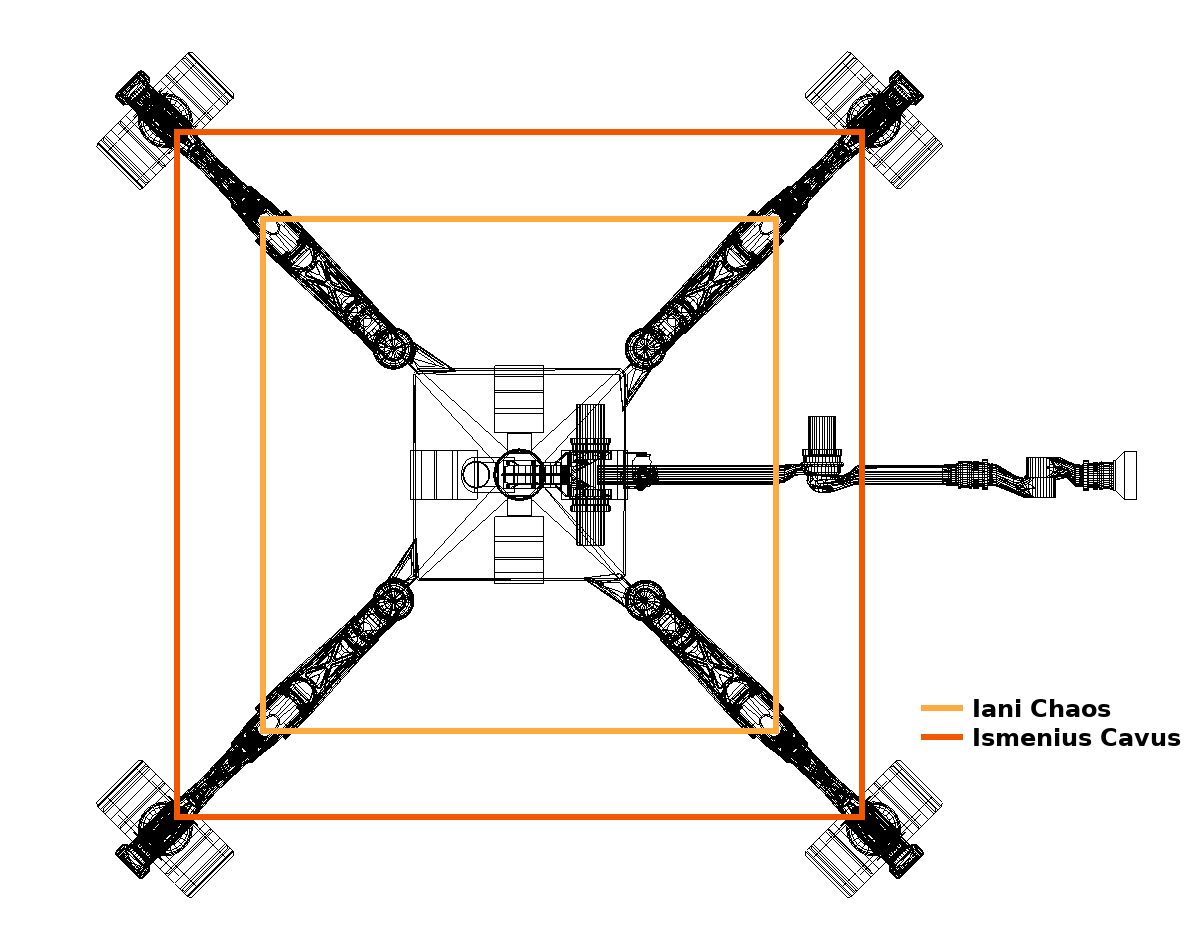
\includegraphics[width=0.7\linewidth]{sections/design/solar-array/images/sa-area-initial-sizes.png}\\
  \caption[Initial solar array sizing for mission sites]
          {Initial \ac{SA} sizing for mission sites. The outlined square areas are equivalent to \ac{SA} areas of \SI{2.7}{m^{2}} for Iani Chaos and \SI{4.8}{m^{2}} for Ismenius Cavus.}
  \label{fig:sa-area-initial-sizes}
\end{figure}

To explain the lack of significant gains with $\beta_{best}$, the generated \ac{SA} energy and maximum traverse durations are plotted in \refFig{fig:plot:iani-chaos-generated-energy-and-max-traverse-durations} and \refFig{fig:plot:ismenius-cavus-generated-energy-and-max-traverse-durations}. At Ismenius Cavus, the \ref{itm:con:daylight_traverse} constraint imposes an upper limit to the maximum traverse durations. The ceiling corresponded to the daylight time that is available for traversing. This results in the \ac{SA} generating excess propulsion energy which cannot be used. As seen in \refFig{fig:plot:sub:iani-chaos-max-traverse-durations}, an inclined \ac{SA} is only relevant during the global dust storm season with a dusty atmosphere of $\tau = 1$. This negligeable advantage results in the limited total traverse gains obtained with $\beta_{best}$. Lack of appreciable traverse distance gains obtained with $\beta_{best}$ is due to the $\tau$ factor applied when evaluating the $H_{\beta}^{worst}$ daily insolation with $\tau = 1$. At high optical opacities, $H_{\beta}^{worst} \approx H_{h}^{worst}$ due to light scattering by airborn Martian dust. This was previously observed in \refFig{fig:plot:insolation-ls}, where diffuse insolation was already the largest component contributing to global insolation at $\tau = 1$. Inclined \ac{SA} surface yield little to no benefits over horizontal surfaces when light is mostly diffuse.

\begin{figure}[h]
\captionsetup[subfigure]{justification=centering}
\vspace{-2ex}
	\centering
    %% setup sizes
    \setlength{\subfigureWidth}{0.50\textwidth}
    \setlength{\graphicsHeight}{80mm}
    %% kill hyper-link highlighting
    \hypersetup{hidelinks=true}%
    %% the figures
    \begin{subfigure}[t]{\subfigureWidth}
        \centering
        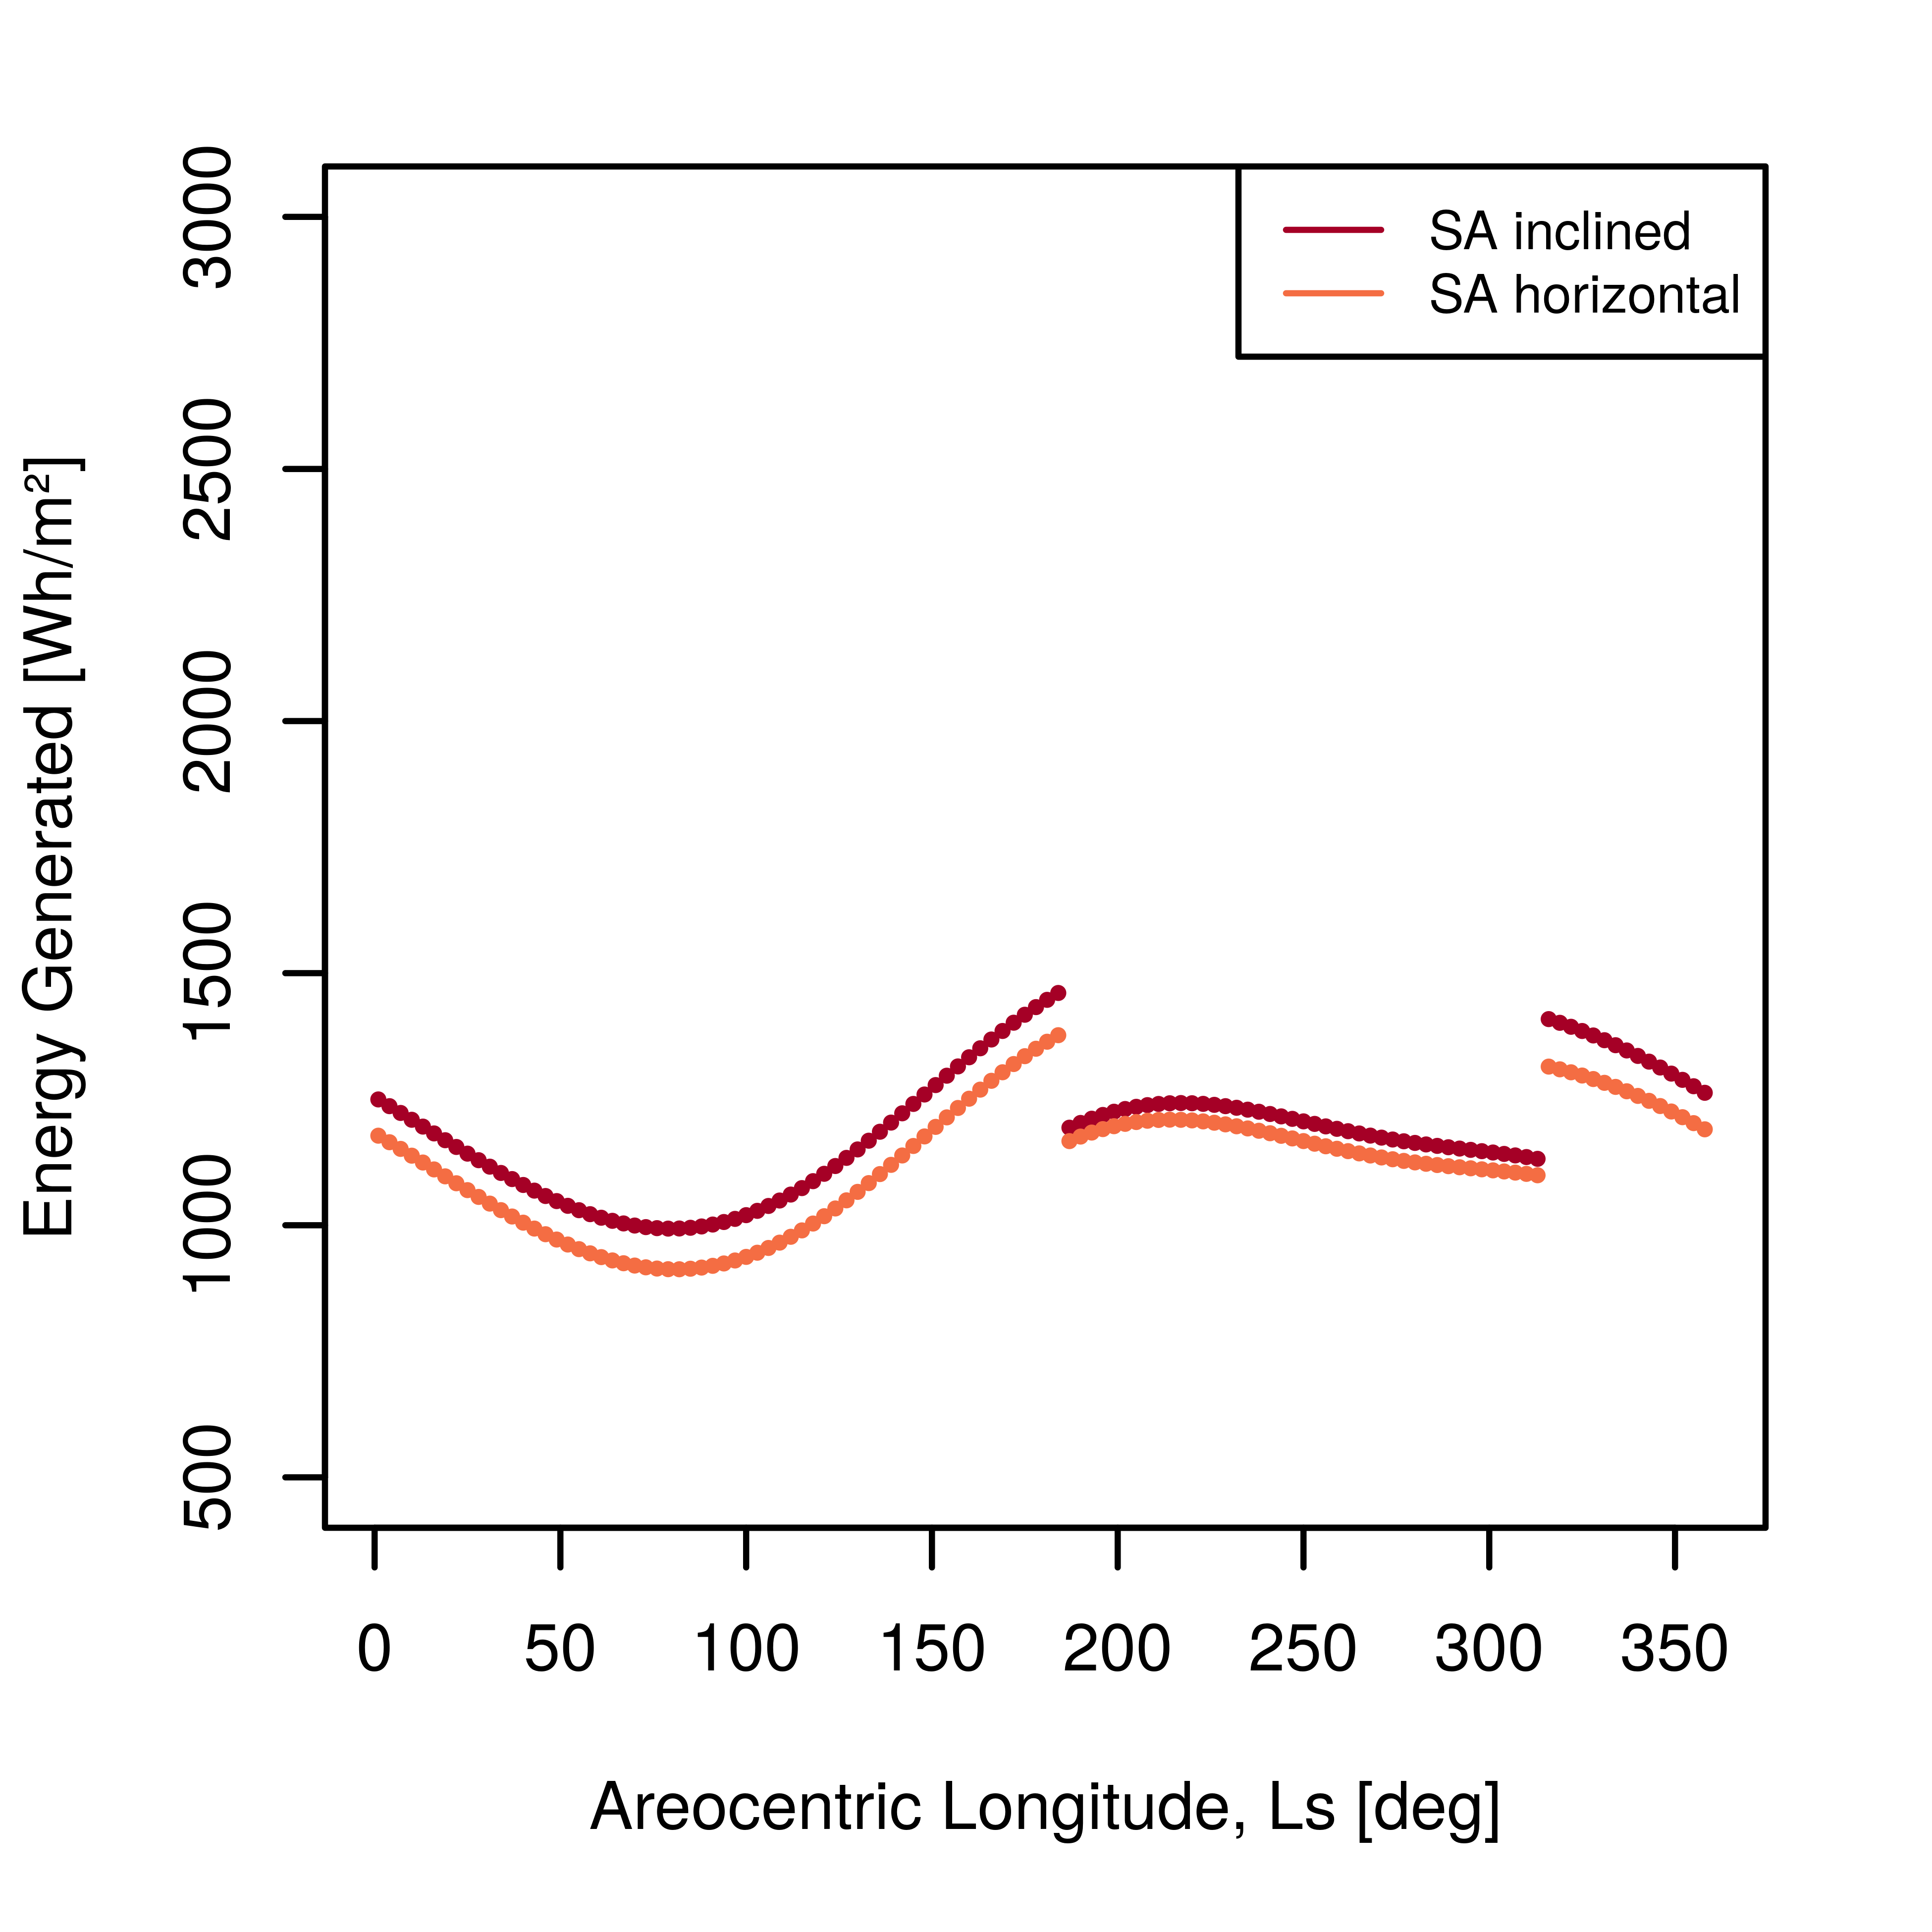
\includegraphics[height=\graphicsHeight]{sections/design/solar-array/plots/ianichaos-daily-generated-energy-for-solar-cell-coverage-area-23m2.png}
        \subcaption{Generated Energy}
        \label{fig:plot:sub:iani-chaos-generated-energy}
    \end{subfigure}\hfill
    \begin{subfigure}[t]{\subfigureWidth}
        \centering
        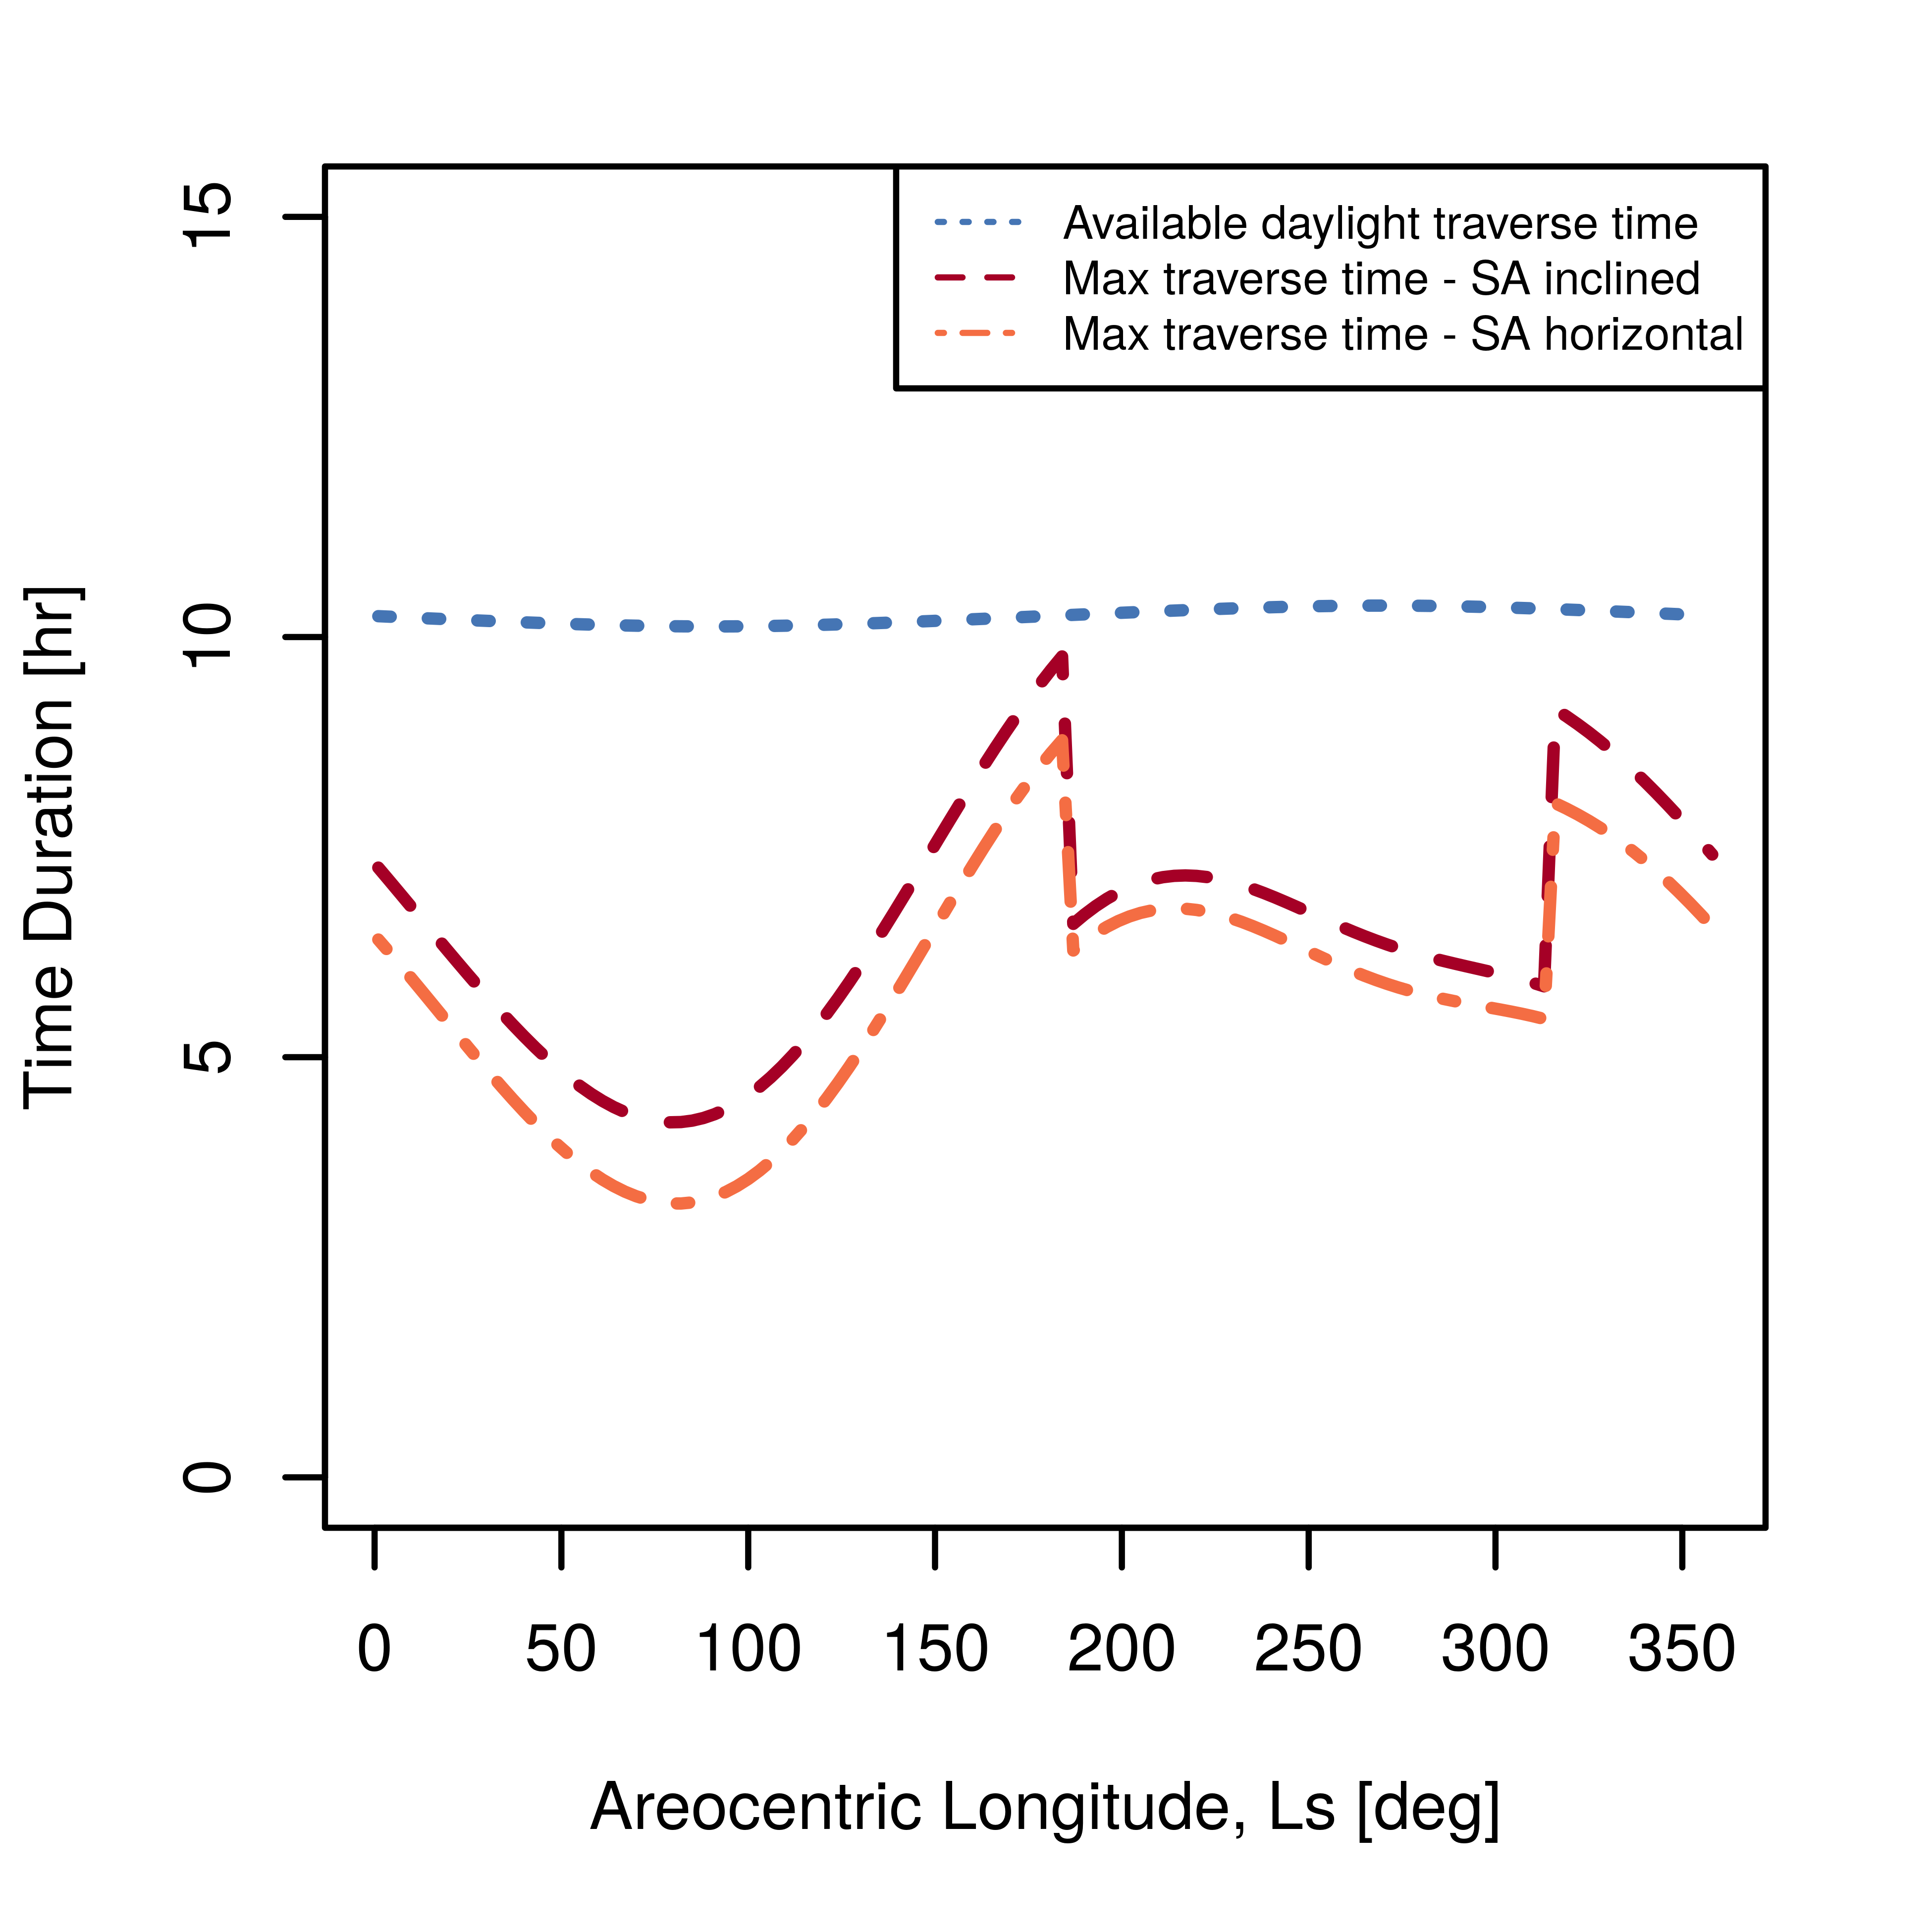
\includegraphics[height=\graphicsHeight]{sections/design/solar-array/plots/ianichaos-75w-max-traverse-durations-for-solar-cell-coverage-area-23m2.png}
  		\subcaption{Maximum Traverse Durations}
		\label{fig:plot:sub:iani-chaos-max-traverse-durations}
	\end{subfigure}\\[0.8ex]
    \caption[Generated energy and maxium flat terrain traverse durations at Iani Chaos]
            {Generated energy and maxium flat terrain traverse duration at Iani Chaos with solar cell coverage area of \SI{2.3}{m^{2}}. Optical depth  $\tau = 1$ was used for global dust storm season ($\SI{185}{\degree} \leq L_{s} \leq \SI{315}{\degree}$) and $\tau = 0.4$ for the remainder of the year. The \textit{available daylight traverse time} corresponds to the amount of daylight hours left in a \textit{Traverse Sol} after subtracting the time taken by non-Traverse modes: \textit{Idle - Day}, \textit{\ac{DTE} Communication}, \textit{Science Stop - Short}, and \textit{Optimal Pose}. The maximum traverse durations for \ac{SA} horizontal do not consider the \textit{Optimal Pose} mode.}
    \label{fig:plot:iani-chaos-generated-energy-and-max-traverse-durations}
\vspace{-2ex}
\end{figure}

\begin{figure}[h]
\captionsetup[subfigure]{justification=centering}
\vspace{-2ex}
	\centering
    %% setup sizes
    \setlength{\subfigureWidth}{0.50\textwidth}
    \setlength{\graphicsHeight}{80mm}
    %% kill hyper-link highlighting
    \hypersetup{hidelinks=true}%
    %% the figures
    \begin{subfigure}[t]{\subfigureWidth}
        \centering
        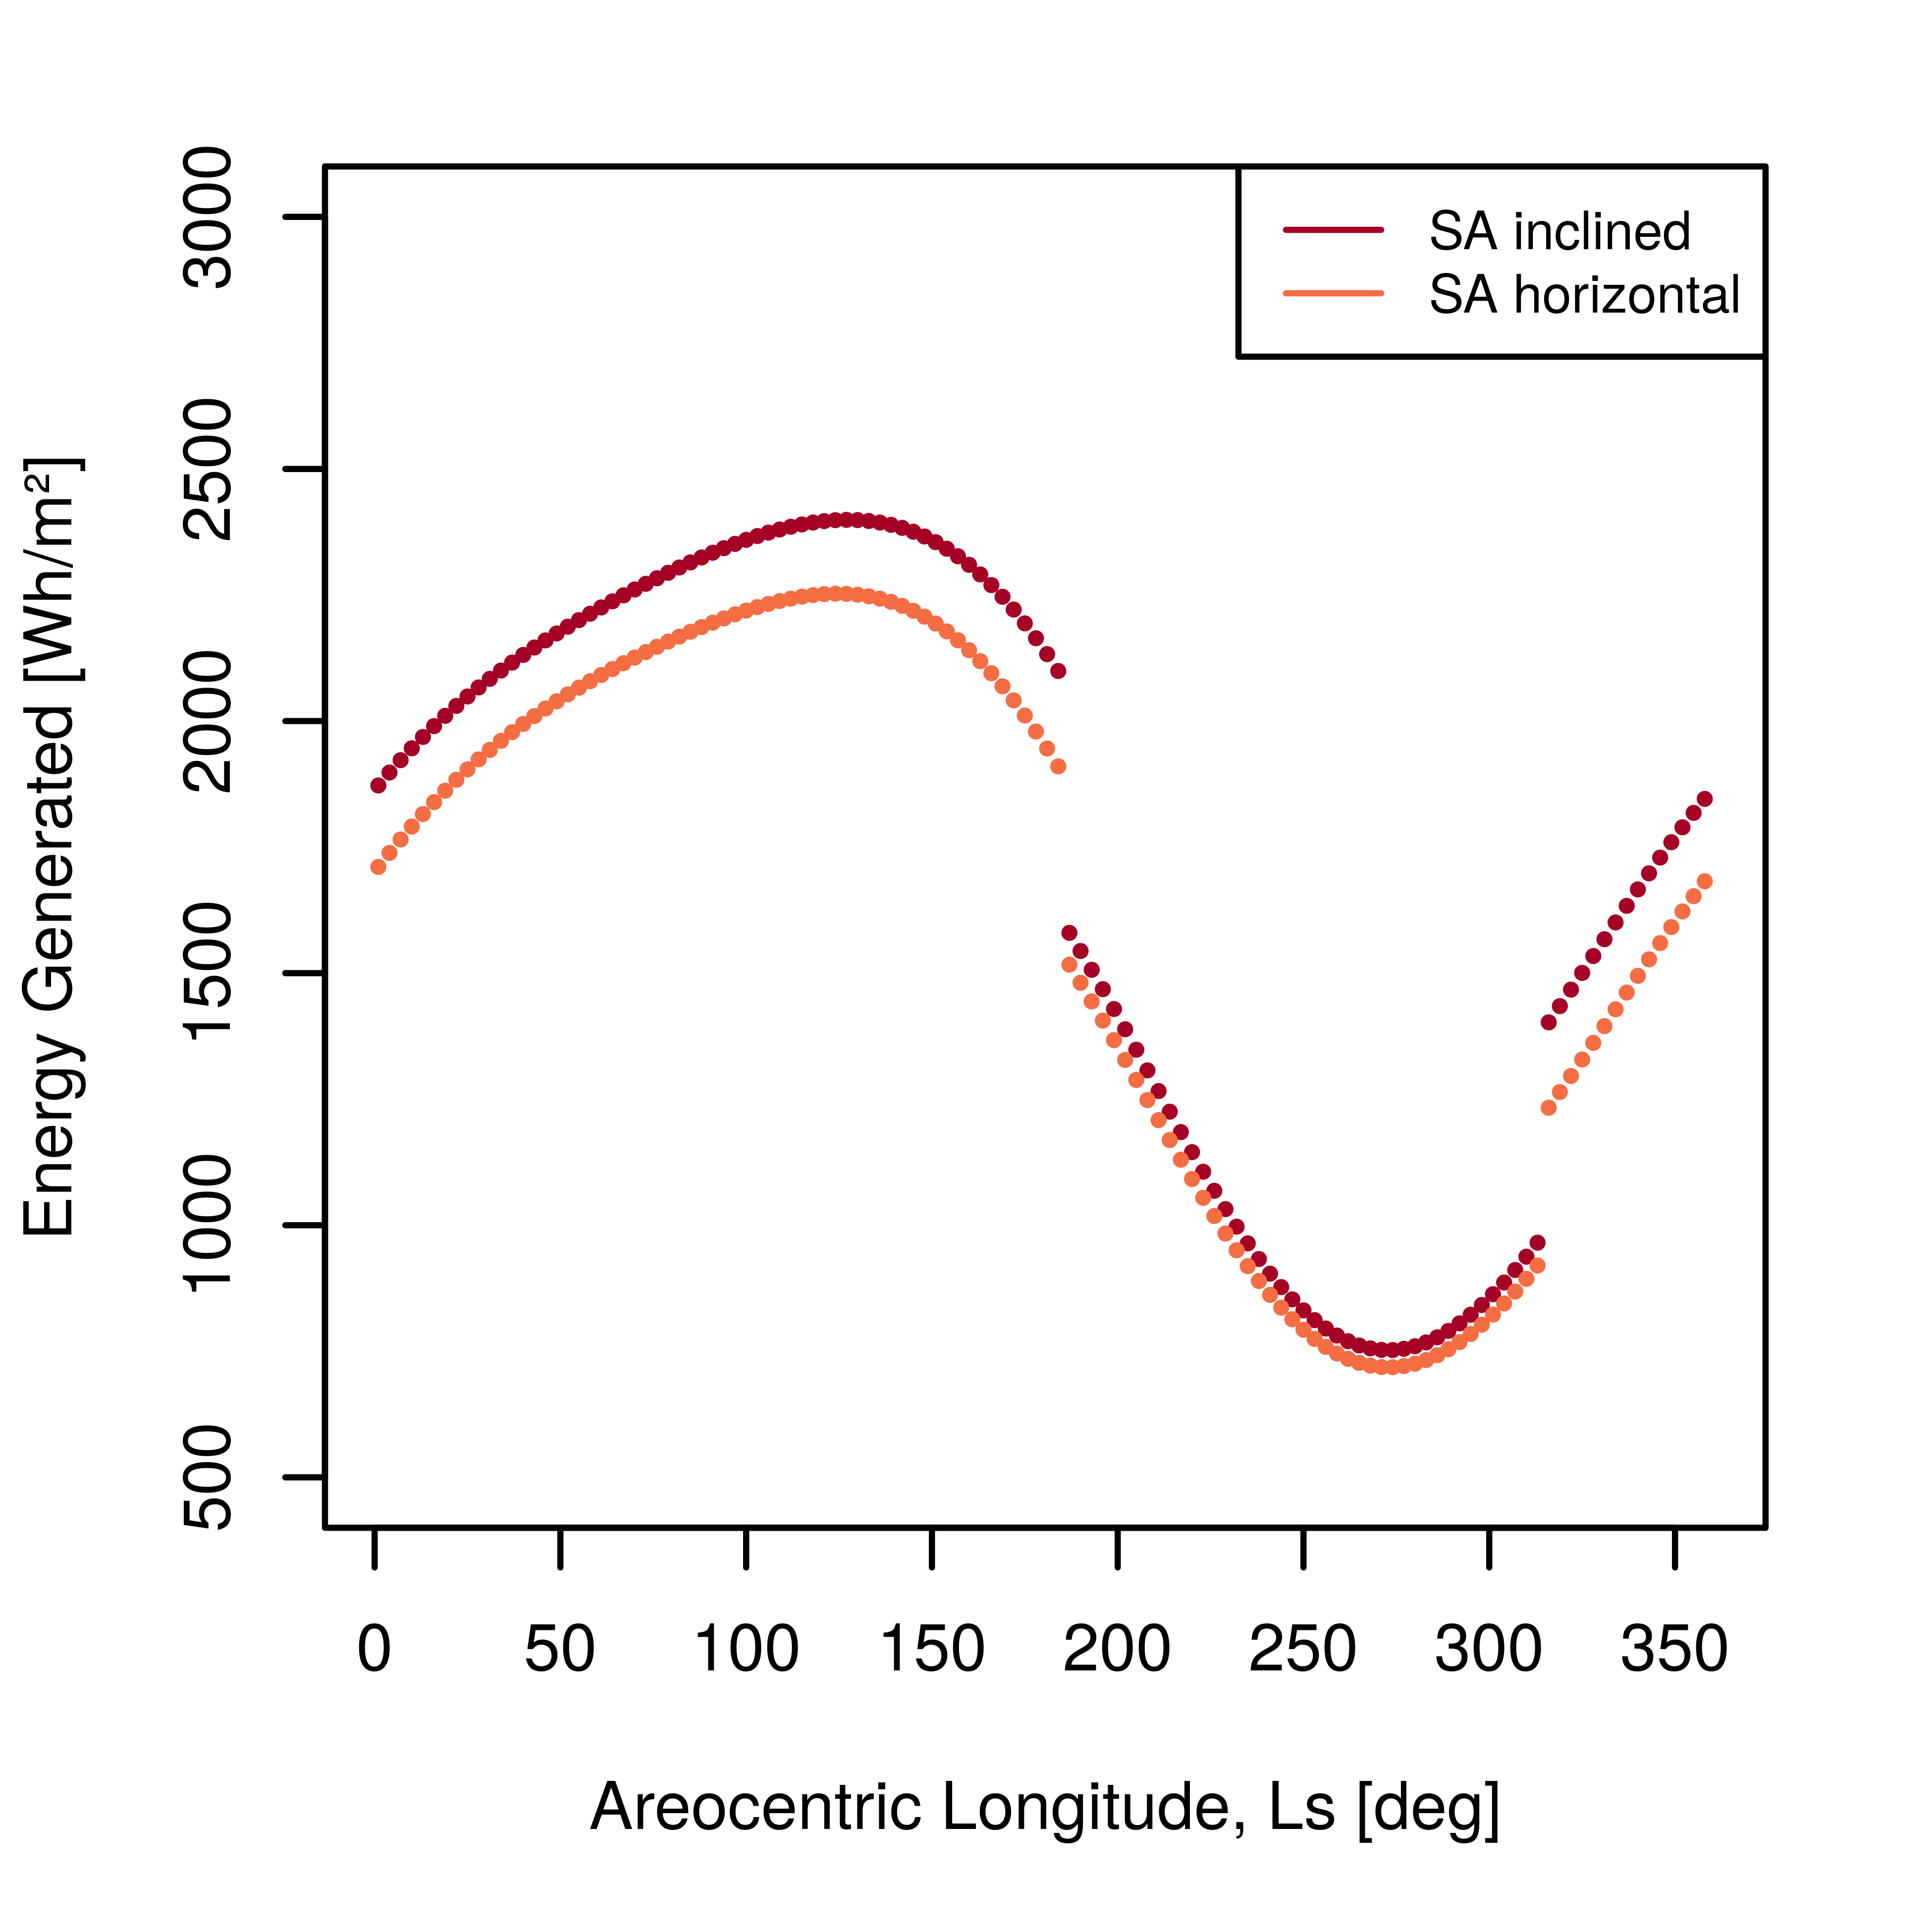
\includegraphics[height=\graphicsHeight]{sections/design/solar-array/plots/ismeniuscavus-daily-generated-energy-for-solar-cell-coverage-area-41m2.png}
        \subcaption{Generated Energy}
        \label{fig:plot:sub:ismenius-cavus-generated-energy}
    \end{subfigure}\hfill
    \begin{subfigure}[t]{\subfigureWidth}
        \centering
        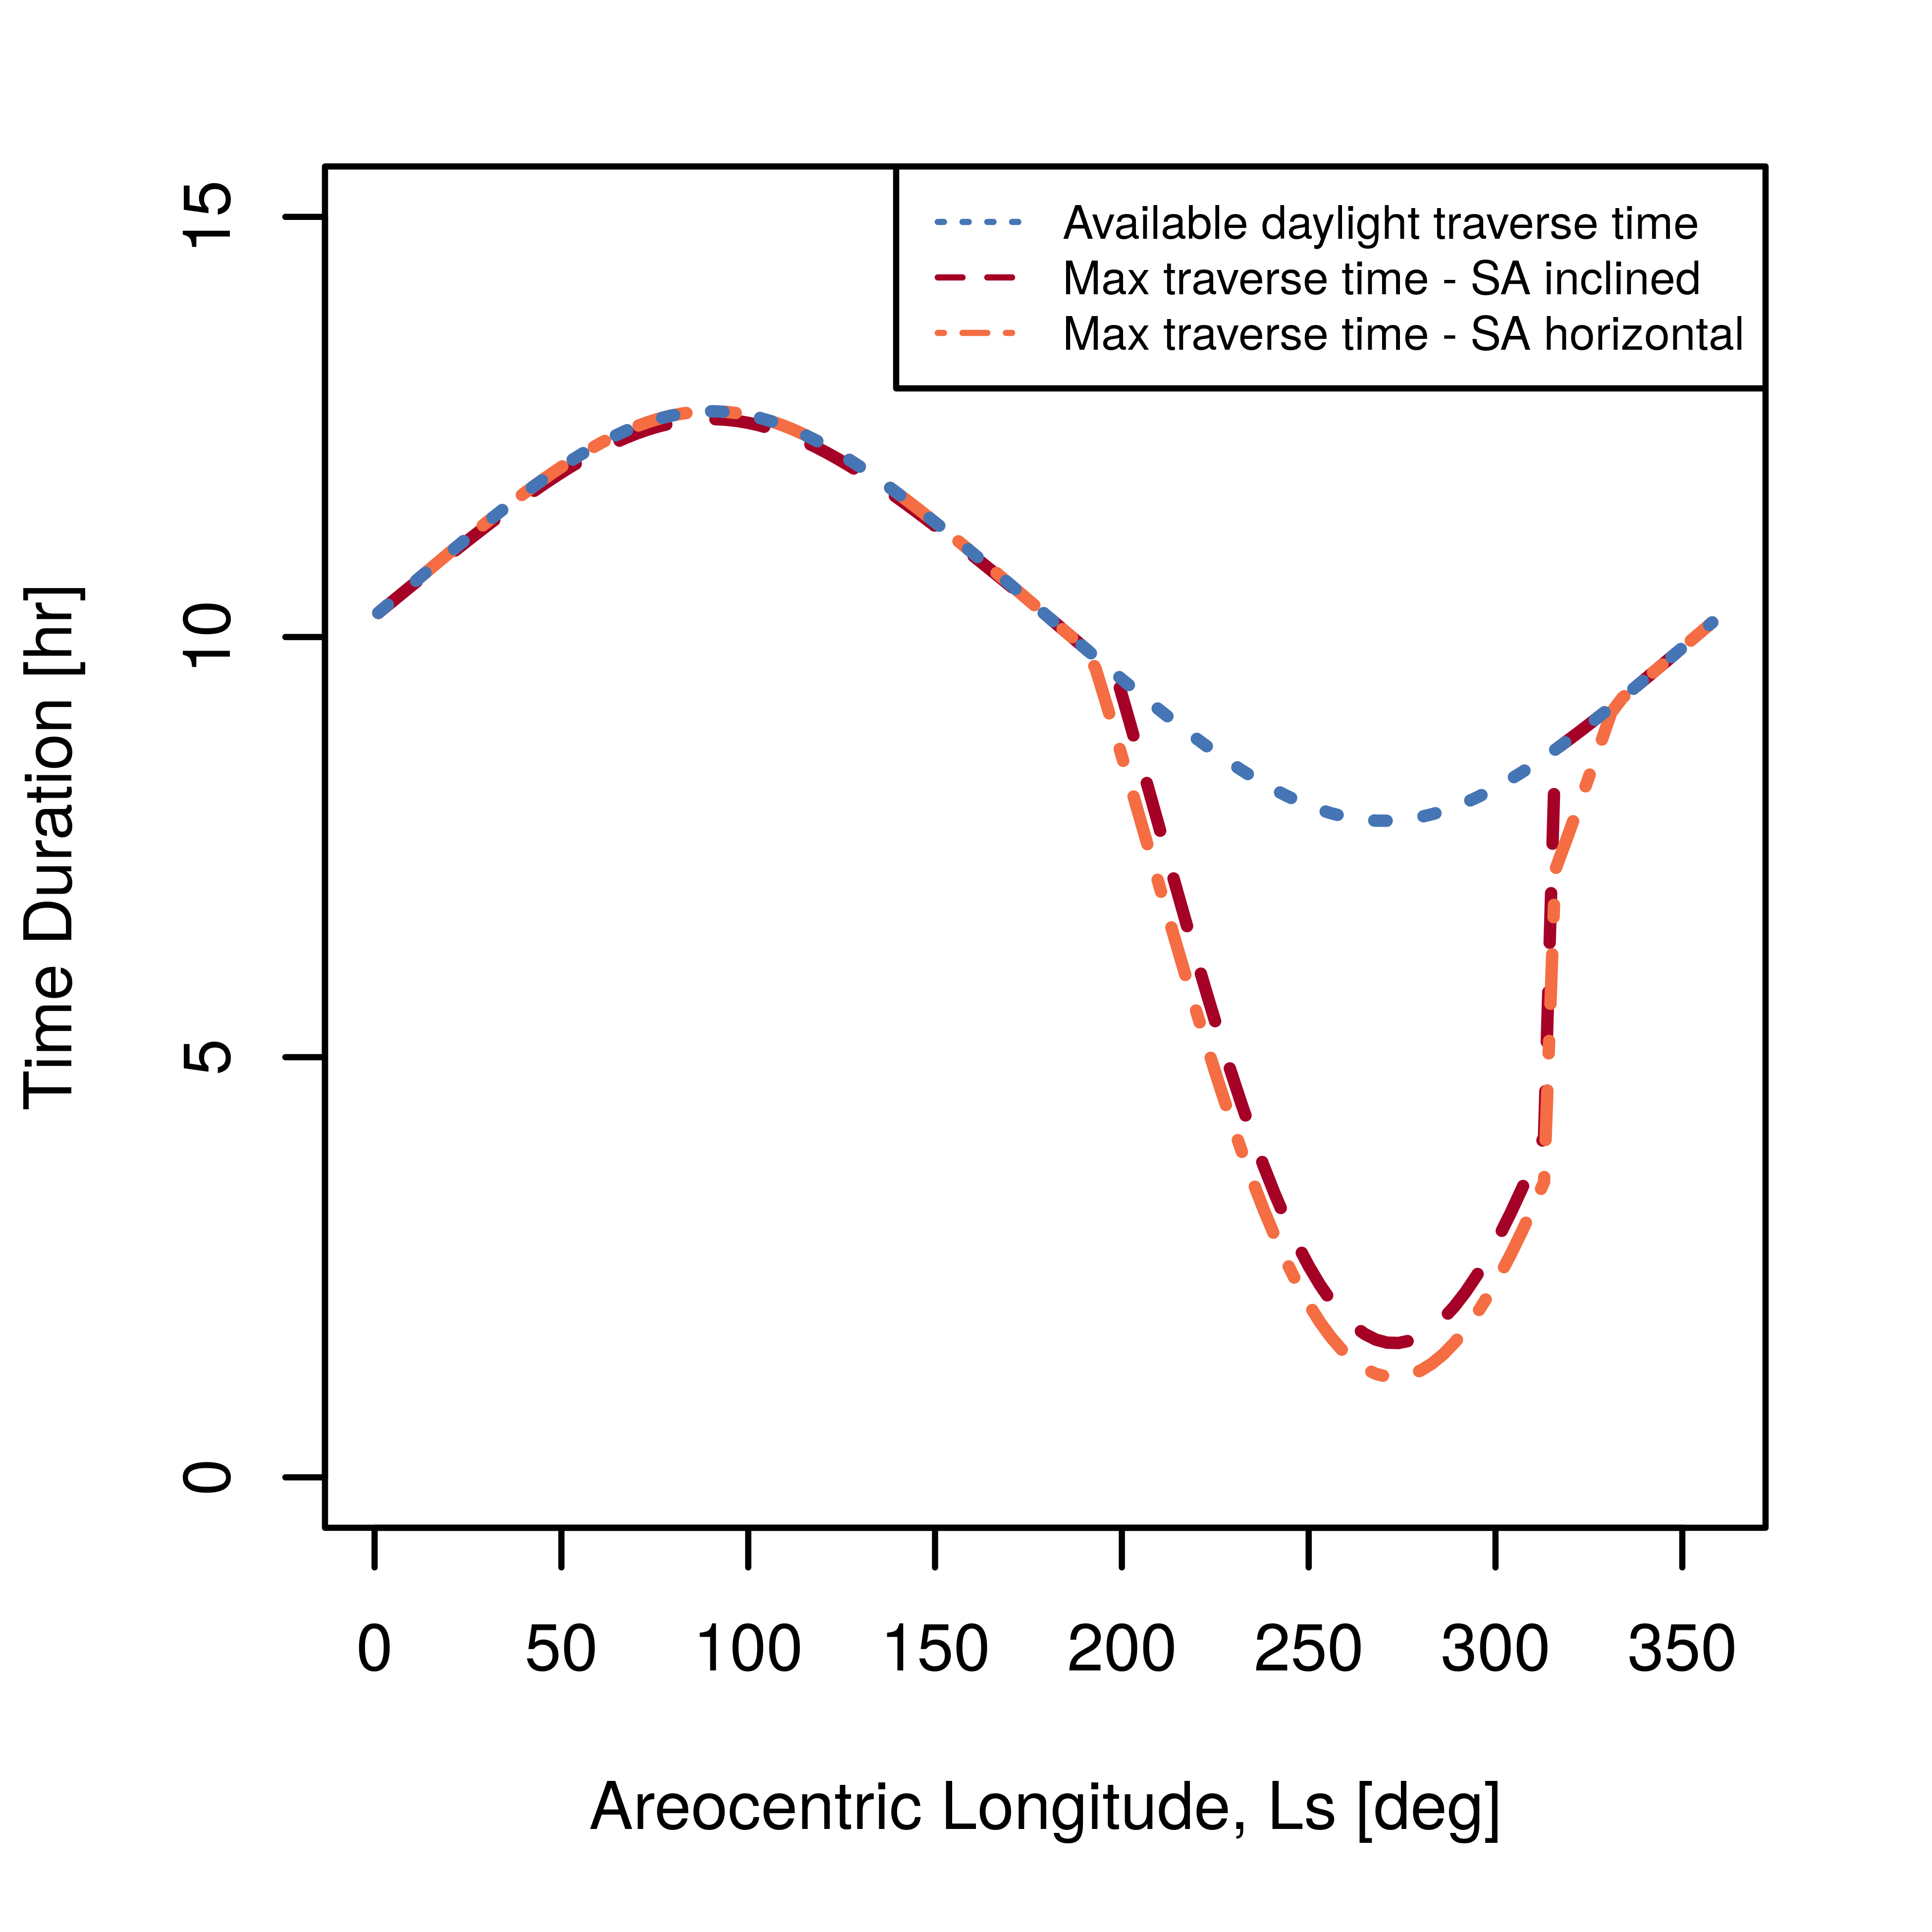
\includegraphics[height=\graphicsHeight]{sections/design/solar-array/plots/ismeniuscavus-75w-max-traverse-durations-for-solar-cell-coverage-area-41m2.png}
  		\subcaption{Maximum Traverse Durations}
		\label{fig:plot:sub:ismenius-cavus-max-traverse-durations}
	\end{subfigure}\\[0.8ex]
    \caption[Generated energy and maxium flat terrain traverse durations at Ismenius Cavus]
            {Generated energy and maxium flat terrain traverse duration at Ismenius Cavus with solar cell coverage area of \SI{4.1}{m^{2}}. The same considerations were taken as in Figure \ref{fig:plot:iani-chaos-generated-energy-and-max-traverse-durations}.}
    \label{fig:plot:ismenius-cavus-generated-energy-and-max-traverse-durations}
\vspace{-2ex}
\end{figure}

\clearpage
\ac{SA} sizes of \SI{2.7}{m^{2}} at Iani Chaos and \SI{4.8}{m^{2}} at Ismenius Cavus results in total attainable flat traverse coverages of \SI{48.04}{\kilo\meter} and \SI{64.39}{\kilo\meter} within one \ac{MY}. These performances exceeded by over approximately five- and six-folds the \ref{itm:req:total_distance_flat_terrain} requirement of \SI{10}{\kilo\meter}. With this in mind, \ac{SA} sizing using \refEqn{calc:solar_cell_area_iani_chaos_traverse} and \refEqn{calc:solar_cell_area_ismenius_cavus_traverse} are approached differently. $E_{req}^{worst}$ is changed from energy required for the worst case \textit{Traverse Sol} to energy required for a \textit{Hibernation Sol}. However, to obtain satisfying results the solar power draw required by the \textit{Hibernation mode} needs to be reduced from \SI{18}{\watt} to \SI{17}{\watt} at Iani Chaos and from \SI{18}{\watt} to \SI{15}{\watt} at Ismenius Cavus. Introducing \acp{RHU} is necessary should these revised solar power requirements be unachievable. A single \ac{RHU} provides approximately \SI{1}{\watt} of heat thus one \ac{RHU} would is required at Iani Chaos and three at Ismenius Cavus. Taking into account a \SI{20}{percent} system margin, $E_{req}^{worst}$ becomes \SI{490}{\watt\hour} for a \textit{Hibernation Sol} at Iani Chaos and \SI{432}{\watt\hour} at Ismenius Cavus. Revisting \refEqn{eq:solar_cell_coverage_area} results in the following solar cell coverage areas:


\begin{align}
  \label{calc:solar_cell_area_iani_chaos_hibernation}
  A_{iani} &= \frac{E_{req}^{worst}}{\eta_{EOL} \cdot H_{\beta}^{worst} \cdot PR_{EOL}}\\
           &= \frac{490}{0.22 \cdot 2479 \cdot 0.62}\\
           &= \SI{1.45}{m^{2}}
\end{align}

\begin{align}
  \label{calc:solar_cell_area_ismenius_cavus_hibernation}
  A_{ismenius} &= \frac{E_{req}^{worst}}{\eta_{EOL} \cdot H_{\beta}^{worst} \cdot PR_{EOL}}\\
               &= \frac{432}{0.22 \cdot 1345 \cdot 0.62}\\
               &= \SI{2.35}{m^{2}}
\end{align}

After considering \ref{itm:ass:packing_efficiency}, the \ac{SA} areas are \SI{1.7}{m^{2}} at Iani Chaos with a mass of \SI{6.3}{\kilo\gram} and \SI{2.8}{m^{2}} at Ismenius Cavus with a mass of  \SI{10.4}{\kilo\gram}. The \ref{itm:req:total_distance_flat_terrain} requirement remain satisfied with
a maxmium flat traverse distance coverage of \SI{12}{\kilo\meter} at Iani Chaos and \SI{35}{\kilo\meter} at Ismenius Cavus. \refFig{fig:plot:flat-traverse-gains-for-different-sa-area} compares the gains in flat traverse distance coverage for different solar cell coverage areas and optical depths in order to better appreciate the gains involved. At Iani Chaos, a \SI{34}{\percent} gain in traverse is achieved on a clear day with $\tau = 0.4$. The gain remains significant at \SI{23}{\percent} for a dusty day with $\tau = 1$. At Ismenius cavus, $\tau = 0.4$ and $\tau = 1$ gains are \SI{19}{\percent} and \SI{11}{\percent}, respectively. The maximum daily traverse durations attainable at both sites with their respective solar cell coverage areas are shown in \refFig{fig:plot:final-maximum-traverse-durations-at-missions-sites}. At Iani Chaos, a \SI{34}{\percent} gain in traverse is achieved on a clear day with $\tau = 0.4$. The gain remains significant at \SI{23}{\percent} for a dusty day with $\tau = 1$. At Ismenius cavus, $\tau = 0.4$ and $\tau = 1$ gains are \SI{19}{\percent} and \SI{11}{\percent}, respectively. The maximum daily traverse durations attainable at both sites with their respective solar cell coverage areas are shown in \refFig{fig:plot:final-maximum-traverse-durations-at-missions-sites}.


\begin{figure}[h]
\captionsetup[subfigure]{justification=centering}
\vspace{-2ex}
	\centering
    %% setup sizes
    \setlength{\subfigureWidth}{0.50\textwidth}
    \setlength{\graphicsHeight}{80mm}
    %% kill hyper-link highlighting
    \hypersetup{hidelinks=true}%
    %% the figures
    \begin{subfigure}[t]{\subfigureWidth}
        \centering
        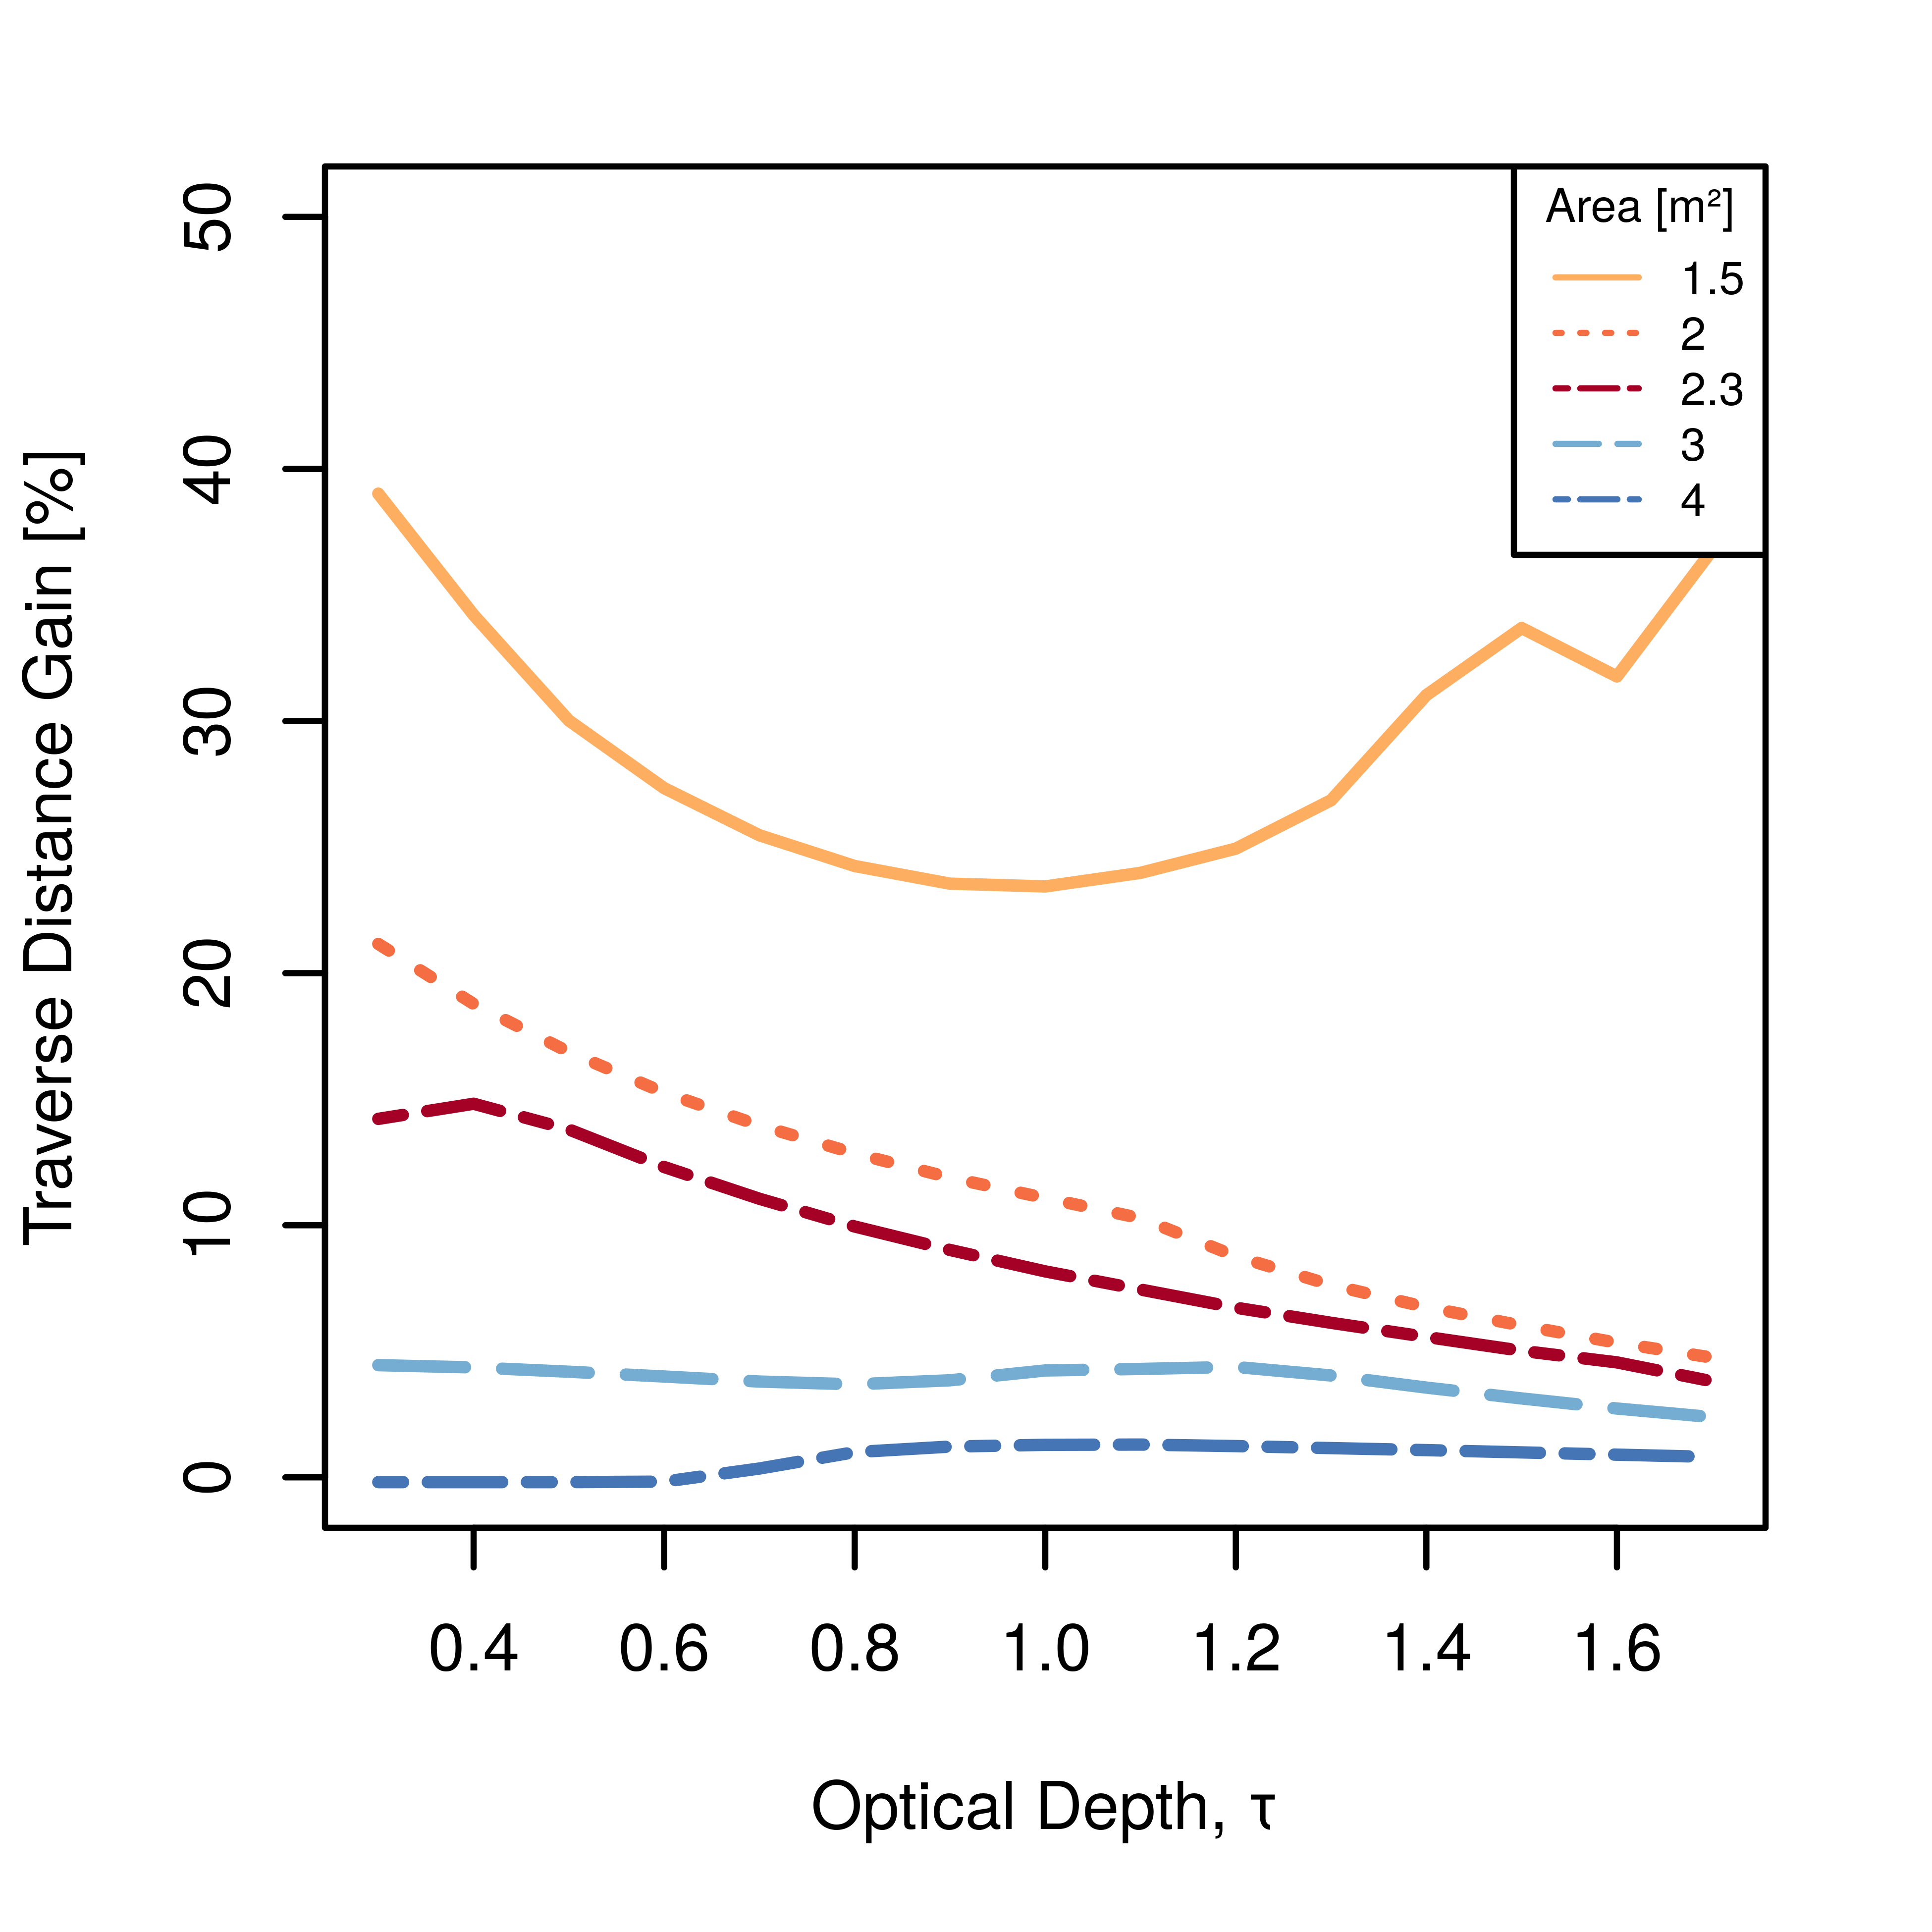
\includegraphics[height=\graphicsHeight]{sections/design/solar-array/plots/ianichaos-75w-traverse-gains-for-different-solar-cell-coverage-areas.png}
  		\subcaption{Iani Chaos}
		\label{fig:plot:sub:ismenius-chaos-flat-traverse-gains-for-different-sa-area}
    \end{subfigure}\hfill
    \begin{subfigure}[t]{\subfigureWidth}
        \centering
        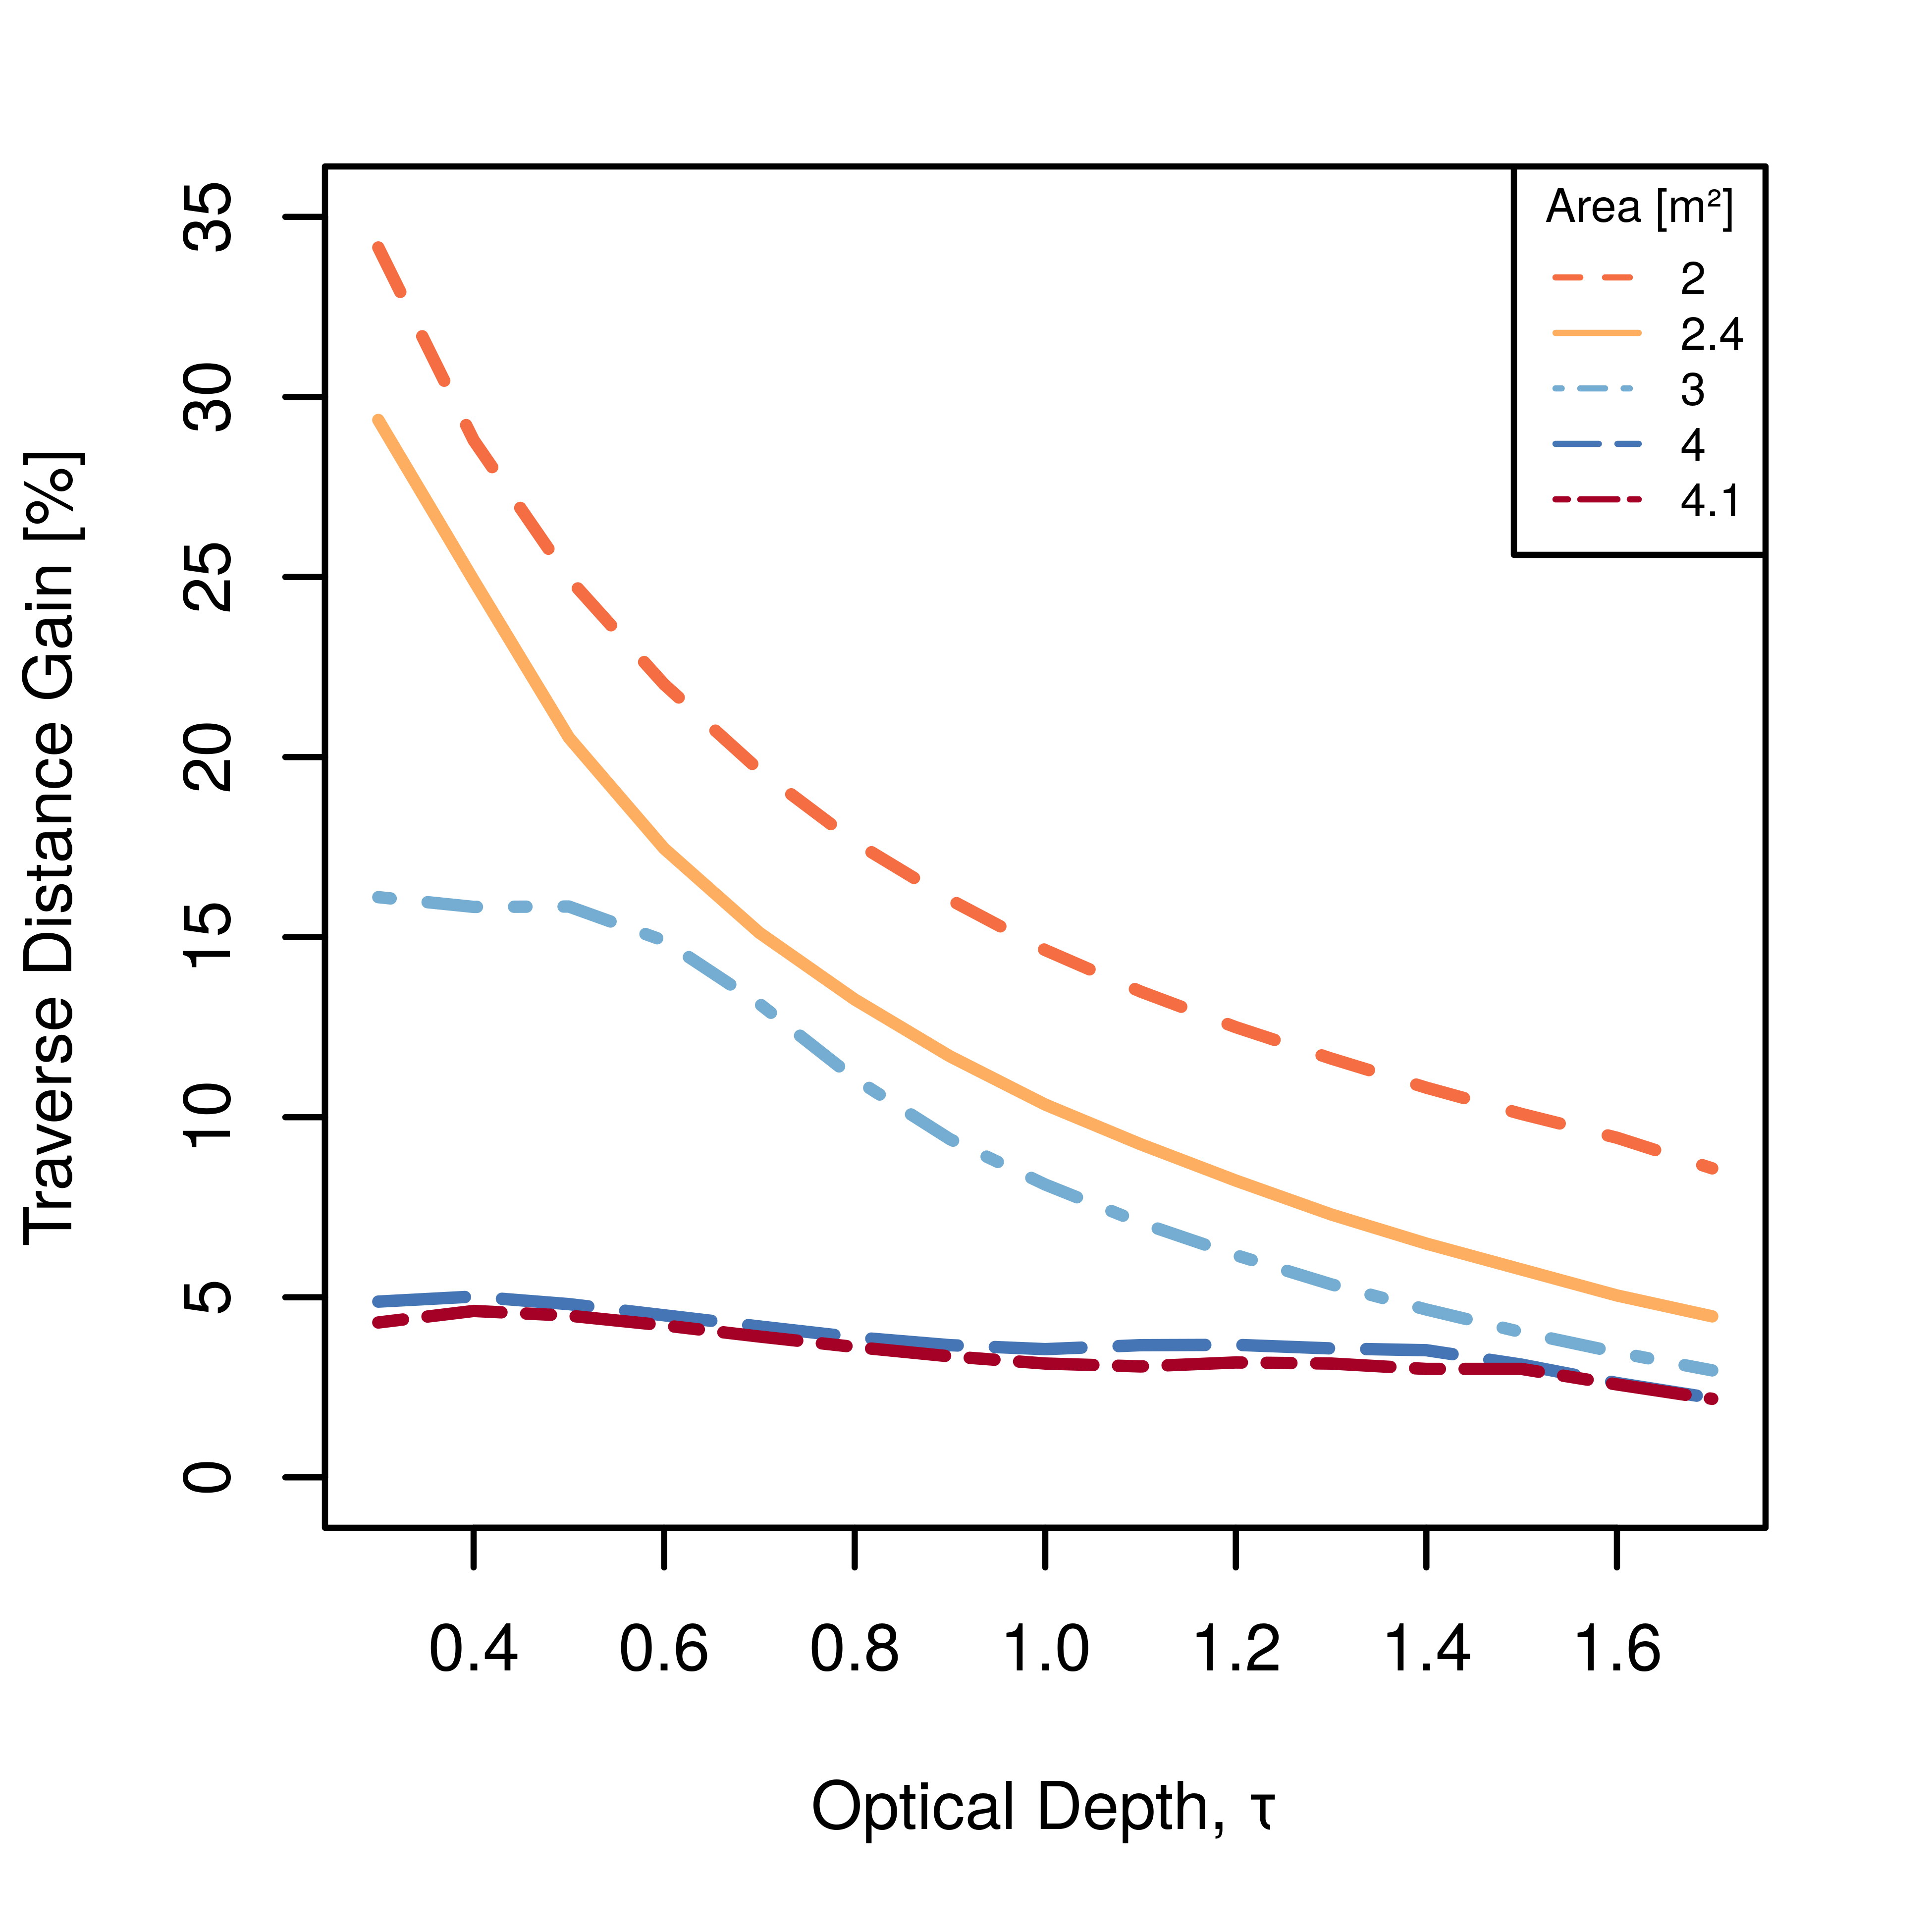
\includegraphics[height=\graphicsHeight]{sections/design/solar-array/plots/ismeniuscavus-75w-traverse-gains-for-different-solar-cell-coverage-areas.png}
  		\subcaption{Ismenius Cavus}
		\label{fig:plot:sub:iani-chaos-flat-traverse-gains-for-different-sa-area}
	\end{subfigure}\\[0.8ex]
    \caption[Flat traverse distance gains at mission sites for different solar cell coverage areas]
            {Flat traverse distance gains at mission sites for different solar cell coverage areas.}
    \label{fig:plot:flat-traverse-gains-for-different-sa-area}
\vspace{-2ex}
\end{figure}


\begin{figure}[h]
\captionsetup[subfigure]{justification=centering}
\vspace{-2ex}
	\centering
    %% setup sizes
    \setlength{\subfigureWidth}{0.50\textwidth}
    \setlength{\graphicsHeight}{80mm}
    %% kill hyper-link highlighting
    \hypersetup{hidelinks=true}%
    %% the figures
    \begin{subfigure}[t]{\subfigureWidth}
        \centering
        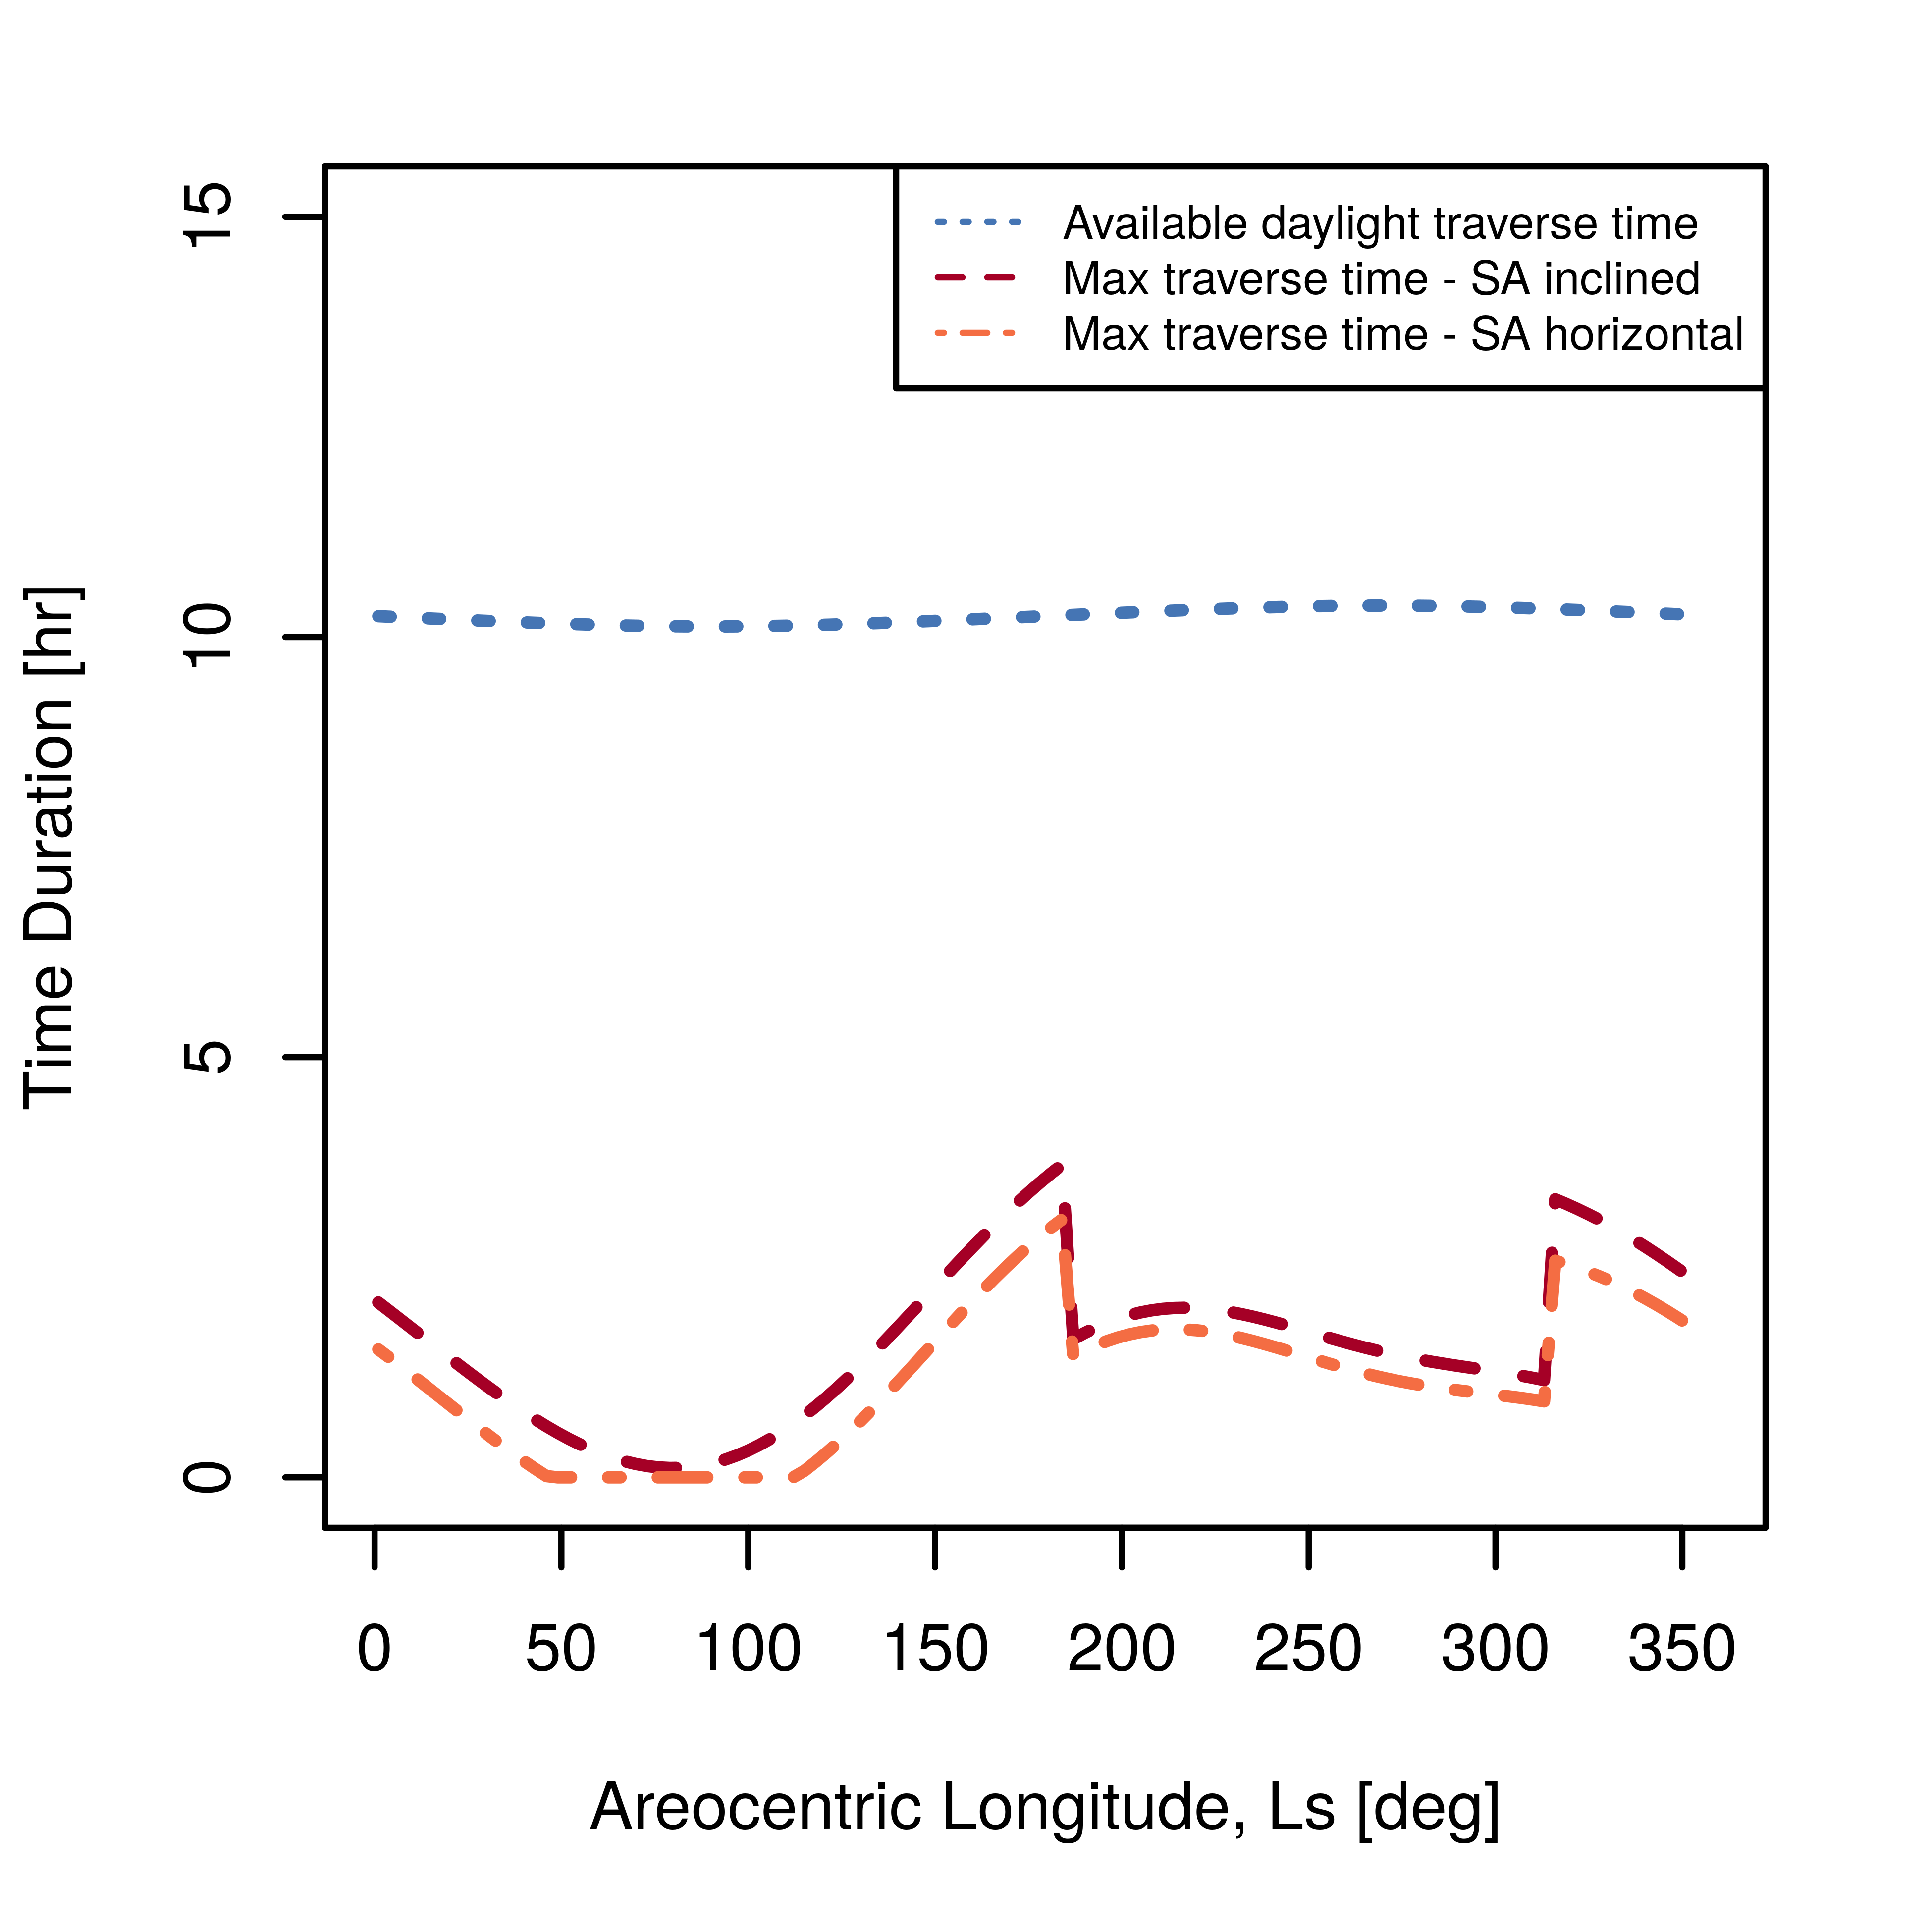
\includegraphics[height=\graphicsHeight]{sections/design/solar-array/plots/ianichaos-75w-max-traverse-durations-for-solar-cell-coverage-area-15m2.png}
  		\subcaption{Iani Chaos, solar cell coverage = \SI{1.5}{m^{2}}}
		\label{fig:plot:sub:final-maximum-traverse-durations-iani-chaos}
    \end{subfigure}\hfill
    \begin{subfigure}[t]{\subfigureWidth}
        \centering
        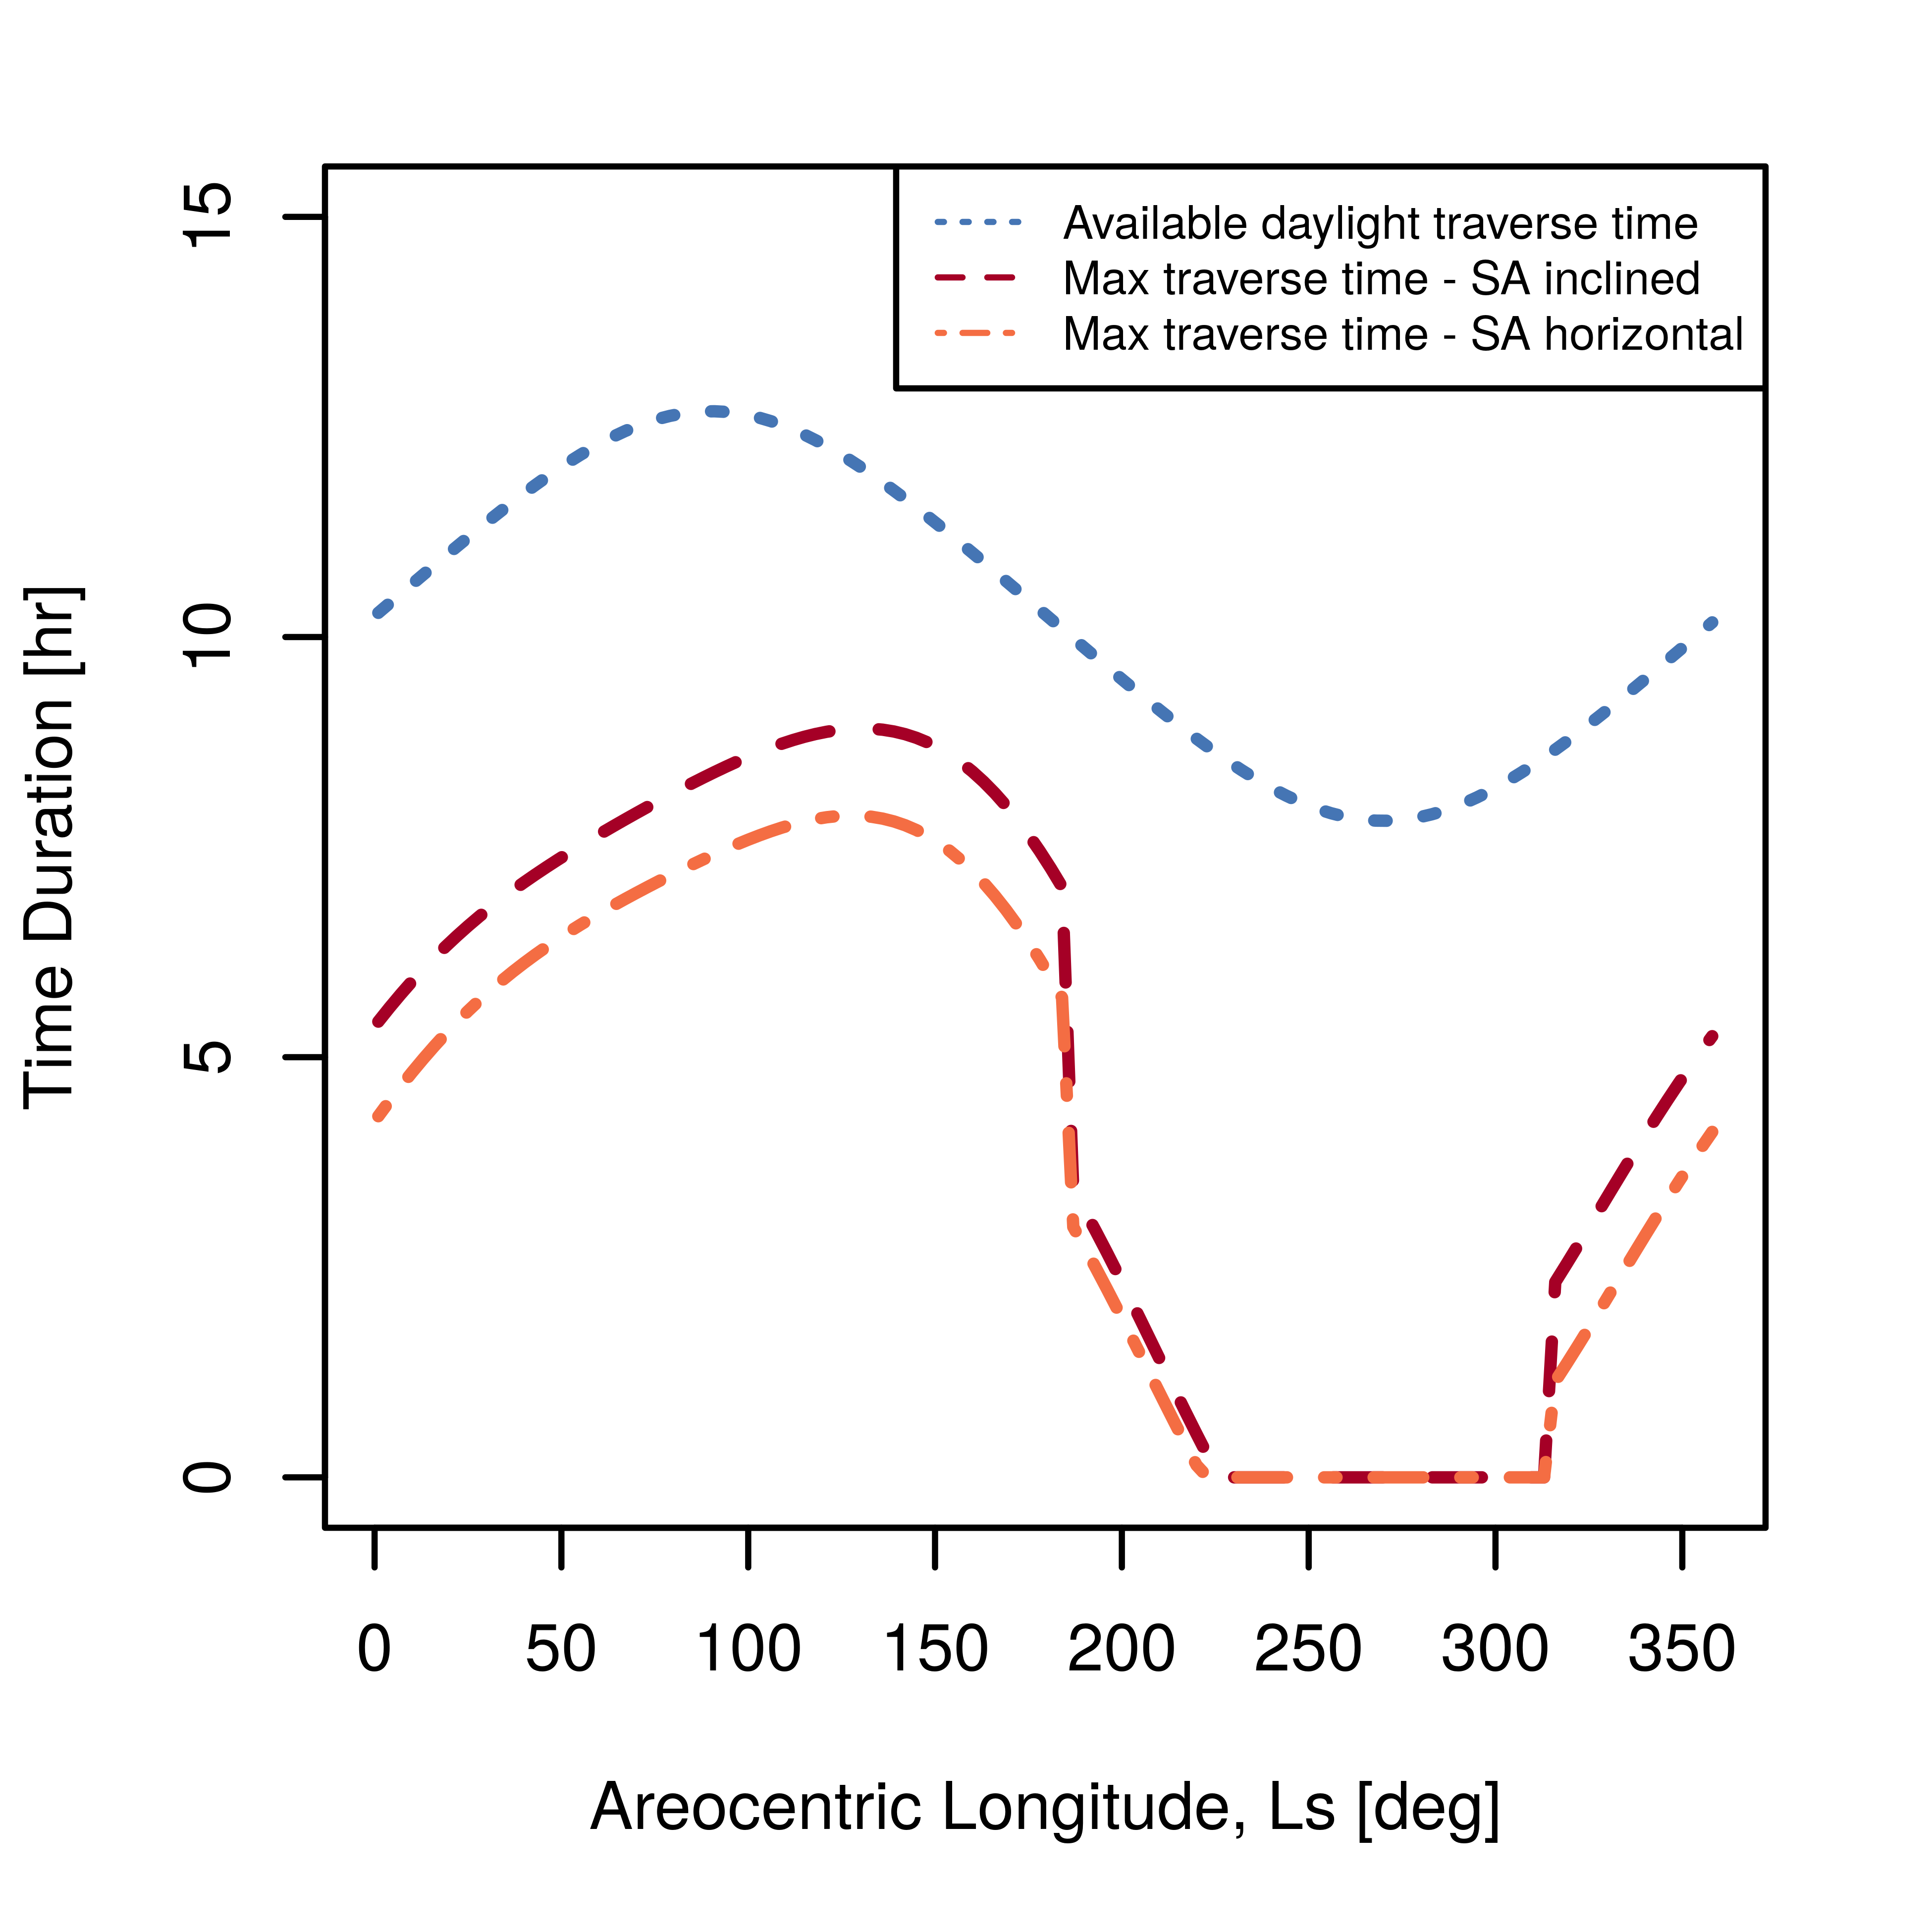
\includegraphics[height=\graphicsHeight]{sections/design/solar-array/plots/ismeniuscavus-75w-max-traverse-durations-for-solar-cell-coverage-area-24m2.png}
  		\subcaption{Ismenius Cavus, solar cell coverage area = \SI{2.4}{m^{2}}}
		\label{fig:plot:sub:final-maximum-traverse-durations-ismenius-cavus}
	\end{subfigure}\\[0.8ex]
    \caption[Maximum traverse durations at mission sites]
            {Maximum traverse durations at mission sites.}
    \label{fig:plot:final-maximum-traverse-durations-at-missions-sites}
\vspace{-2ex}
\end{figure}


%\clearpage
%\subsubsection{Battery}
%\todo[inline]{\textbf{TODO:} Battery size based on energy required to keep the rover Warm through the night. Check if the calculated size satisfies the hibernation requirement. If not, resize.}

\clearpage
\subsection{Baseline Design}
As per \ref{itm:dd:shadowing}, the rover's body is redesigned in order to minimize shadowing events. A pyramid shaped body continuously casts a shadow on a surrounding \ac{SA} with an exception during solar noon. Even then, it is likely that the rover would be tilted to achieve $\beta_{best}$ and thus still be subject to shadowing. The redesigned body shown in \refFig{fig:rover-body-redesign} opts for a box shape with a flat top on which one of the \ac{SA} panels rests. The dimension of the redesigned body is $\SI{65}{\centi\meter}\times\SI{65}{\centi\meter}\times\SI{63}{\centi\meter}$ with the base preserving the pyramid's base area in order to minimize changes in sizing dependent considerations.

\begin{figure}[h]
\captionsetup[subfigure]{justification=centering}
\vspace{-2ex}
	\centering
    %% setup sizes
    \setlength{\subfigureWidth}{0.50\textwidth}
    \setlength{\graphicsHeight}{48mm}
    %% kill hyper-link highlighting
    \hypersetup{hidelinks=true}%
    %% the figures
    \begin{subfigure}[t]{\subfigureWidth}
        \centering
        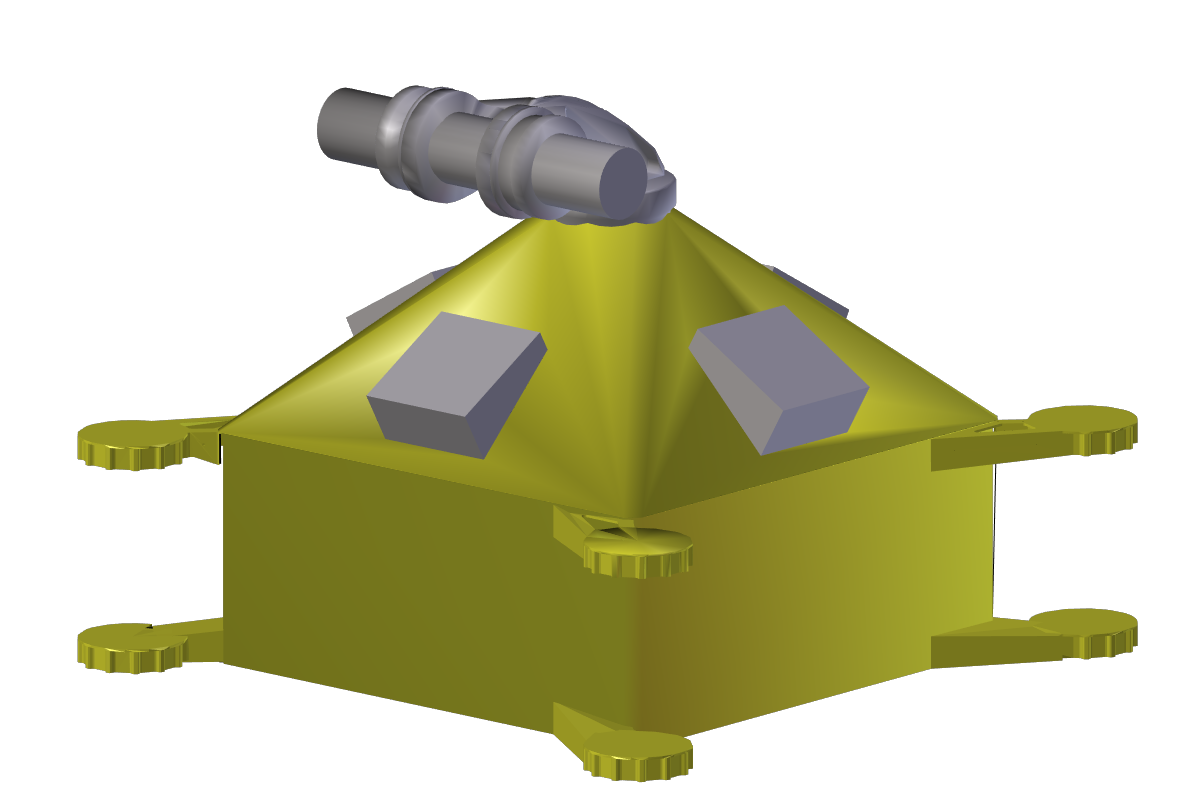
\includegraphics[height=\graphicsHeight]{sections/design/solar-array/images/body-before.png}
        \subcaption{Before}
		\label{fig:sub:rover-body-redesign-before}
    \end{subfigure}\hfill
    \begin{subfigure}[t]{\subfigureWidth}
        \centering
        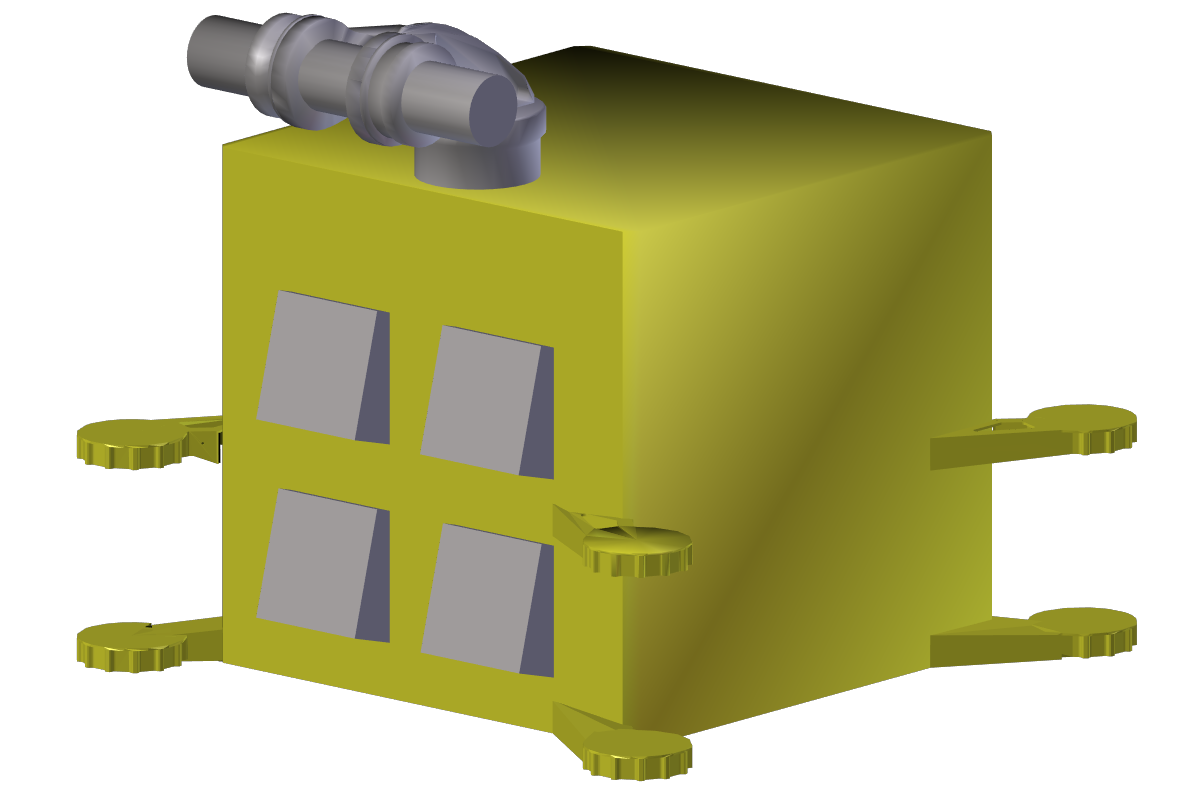
\includegraphics[height=\graphicsHeight]{sections/design/solar-array/images/body-after.png}
  		\subcaption{After}
		\label{fig:sub:rover-body-redesign-after}
	\end{subfigure}\\[0.8ex]
    \caption[Rover body redesign]
            {Rover body redesign.}
    \label{fig:rover-body-redesign}
\vspace{-2ex}
\end{figure}

Placing the four \acp{PLI} is driven by \ref{itm:dd:four_plis} and shown in \refFig{fig:sub:rover-body-redesign-after}. They are stored in the front of body and are accessible by the rover's robotic arm. As will be seen further in this section, access to the body's other faces is obstructed by the \ac{SA} panels. Spacing is left between the \acp{PLI} and the top of the body to allow for instruments. The \acp{PLI} are oriented upwards by \SI{15}{\degree} in order to compensate against possible forward tilts from the rover repositioning itself to attain $\beta_{best}$. The upward tilt of the \ac{PLI} has the added benefit of facilitated access for the robotic arm. The position of the latter is shifted towards the front in order to maximize the surface area that can be uninterruptedly covered by solar cells. As per \ref{itm:dd:unobstructed}, the movemement range of the suspension system must remain unobstructed. The height of the redesigned body is such that the deployed \ac{SA} panels are kept above the legs for any configuration of the active suspension system. This is demonstrated in \refFig{fig:rover-body-redesign-stowed-legs} where the rover's stowed posture results in its knees reaching their highest point.

\begin{figure}[h]
\captionsetup[subfigure]{justification=centering}
\vspace{-2ex}
	\centering
    %% setup sizes
    \setlength{\subfigureWidth}{0.50\textwidth}
    \setlength{\graphicsHeight}{50mm}
    %% kill hyper-link highlighting
    \hypersetup{hidelinks=true}%
    %% the figures
    \begin{subfigure}[t]{\subfigureWidth}
        \centering
        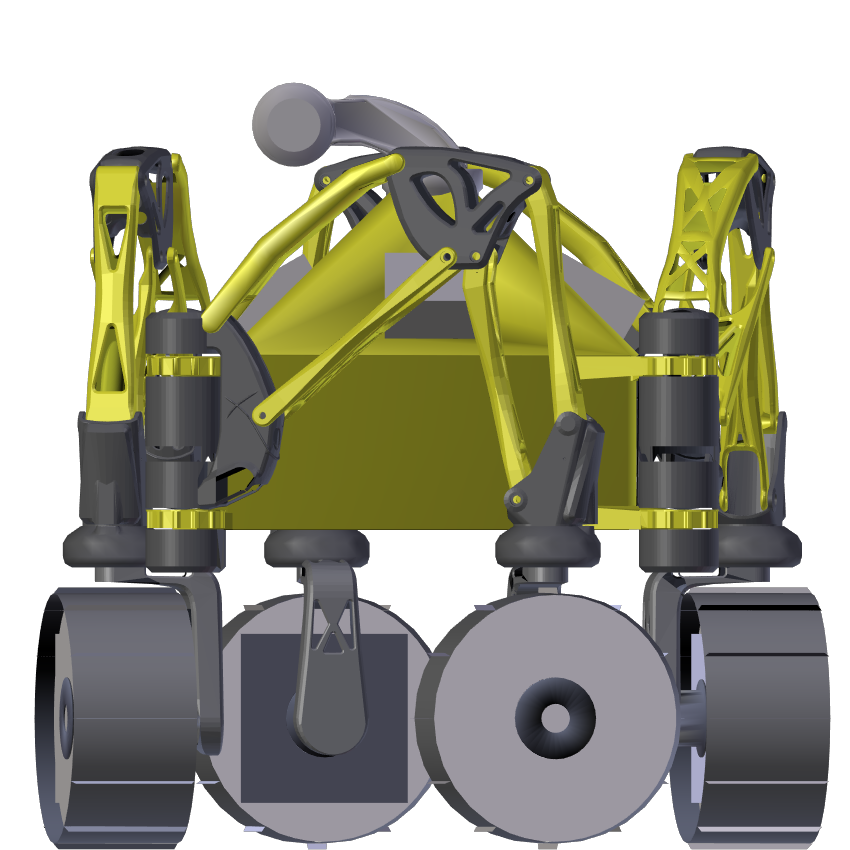
\includegraphics[height=\graphicsHeight]{sections/design/solar-array/images/stowed-body-pyramid.png}
        \subcaption{Before}
		\label{fig:sub:rover-body-redesign-stowed-before}
    \end{subfigure}\hfill
    \begin{subfigure}[t]{\subfigureWidth}
        \centering
        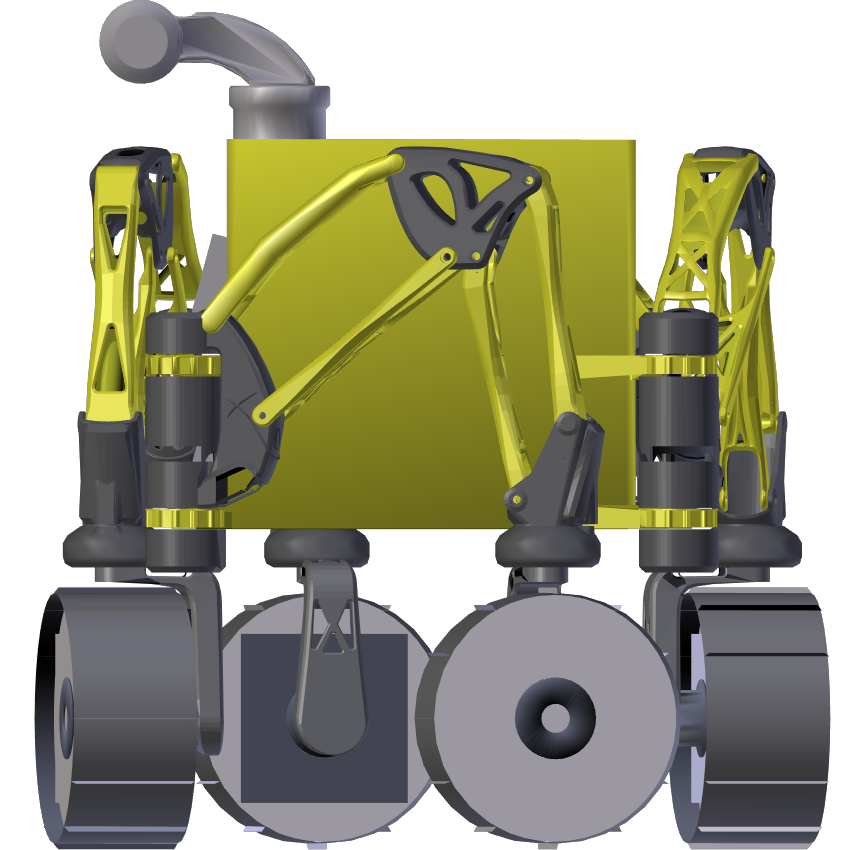
\includegraphics[height=\graphicsHeight]{sections/design/solar-array/images/stowed-body-box.png}
  		\subcaption{After}
		\label{fig:sub:rover-body-redesign-stowed-legs-after}
	\end{subfigure}\\[0.8ex]
    \caption[Rover body redesign with stowed legs]
            {Rover body redesign with stowed legs.}
    \label{fig:rover-body-redesign-stowed-legs}
\vspace{-2ex}
\end{figure}


Folded and deployed \ac{SA} panels are show in \refFig{fig:solar-array-on-rover-iani-chaos} and \refFig{fig:solar-array-on-ismenius-cavus-chaos} as they would appear mounted on top of the rover's body for different mission sites. When folded, the port, starboard, and stern panels do not lay on top of the rover's body and are instead kept upright normal to the body's top surface. The base of the robotic arm occupies an area of the body's surface that prevents the panels from folding in completely. Shifting the robotic arm onto its own support in front of the body would resolve this but prevents the rover's front right leg from assuming its stowed position.

\vspace{0.5cm}

\begin{figure}[h]
\captionsetup[subfigure]{justification=centering}
\vspace{-2ex}
	\centering
    %% setup sizes
    \setlength{\subfigureWidth}{0.50\textwidth}
    \setlength{\graphicsHeight}{53mm}
    %% kill hyper-link highlighting
    \hypersetup{hidelinks=true}%
    %% the figures
    \begin{subfigure}[t]{\subfigureWidth}
        \centering
        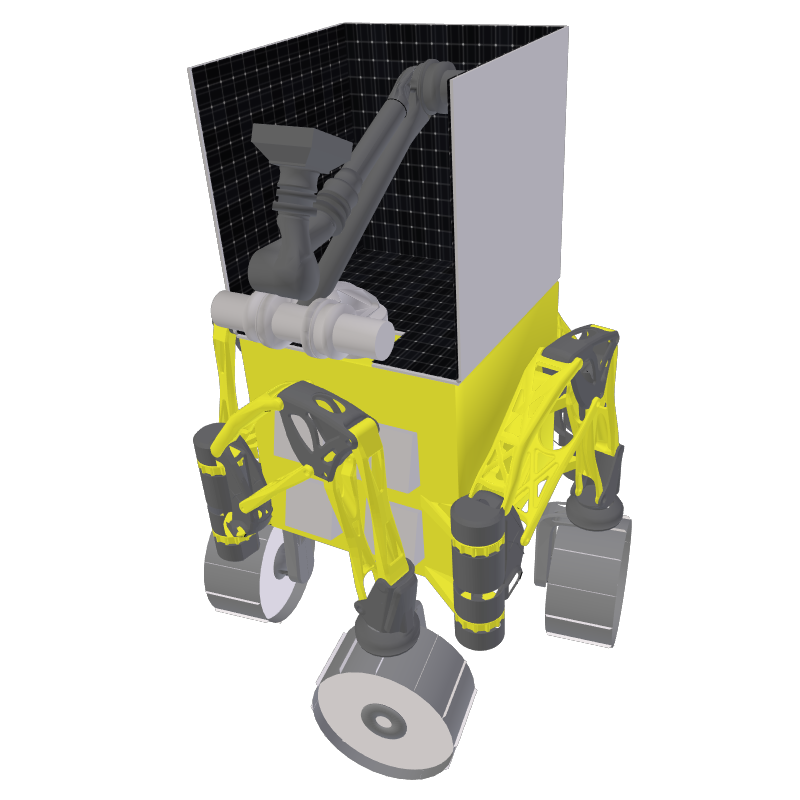
\includegraphics[height=\graphicsHeight]{sections/design/solar-array/images/iani-chaos-stowed.png}
  		\subcaption{Folded on stowed rover}
		\label{fig:sub:solar-array-on-rover-for-iani-chaos-stowed}
    \end{subfigure}\hfill
    \begin{subfigure}[t]{\subfigureWidth}
        \centering
        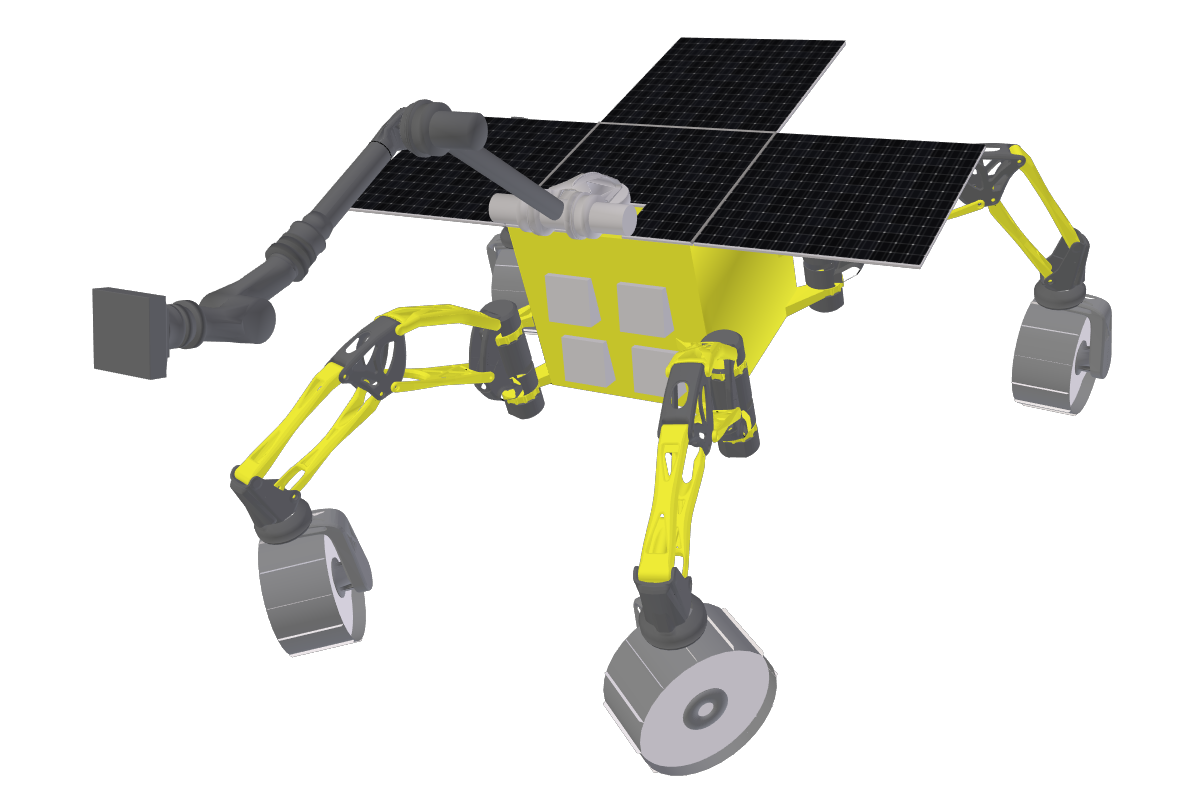
\includegraphics[height=\graphicsHeight]{sections/design/solar-array/images/iani-chaos-10deg-pitch.png}
  		\subcaption{Deployed on rover with \SI{10}{\degree} pitch forward}
		\label{fig:sub:solar-array-on-rover-for-iani-chaos-deployed}
	\end{subfigure}\\[0.8ex]
    \caption[Solar array on rover for Iani Chaos deployment]
            {\ac{SA} on rover for Iani Chaos deployment.}
    \label{fig:solar-array-on-rover-iani-chaos}
\vspace{-2ex}
\end{figure}

\vspace{0.5cm}

The folded configurations shown in \refFig{fig:sub:solar-array-on-rover-for-iani-chaos-stowed} and \refFig{fig:sub:solar-array-on-rover-for-iani-chaos-deployed} were accepted considering that the gain in height does not add much to what is already imposed by the stowed robotic arm. In terms of compactness, a preferable configuration would be one in which all panels are folded in and the robotic arm is stowed against the front side of the body. However, supporting already existing rover postures is preferred. Future design iterations of the stowed configuration for both the robotic arm and the \ac{SA} panels should prioritize compactness based on a \ac{LV} payload capacity and the rover's lander constraints.

\vspace{0.5cm}

\begin{figure}[h]
\captionsetup[subfigure]{justification=centering}
\vspace{-2ex}
	\centering
    %% setup sizes
    \setlength{\subfigureWidth}{0.50\textwidth}
    \setlength{\graphicsHeight}{53mm}
    %% kill hyper-link highlighting
    \hypersetup{hidelinks=true}%
    %% the figures
    \begin{subfigure}[t]{\subfigureWidth}
        \centering
        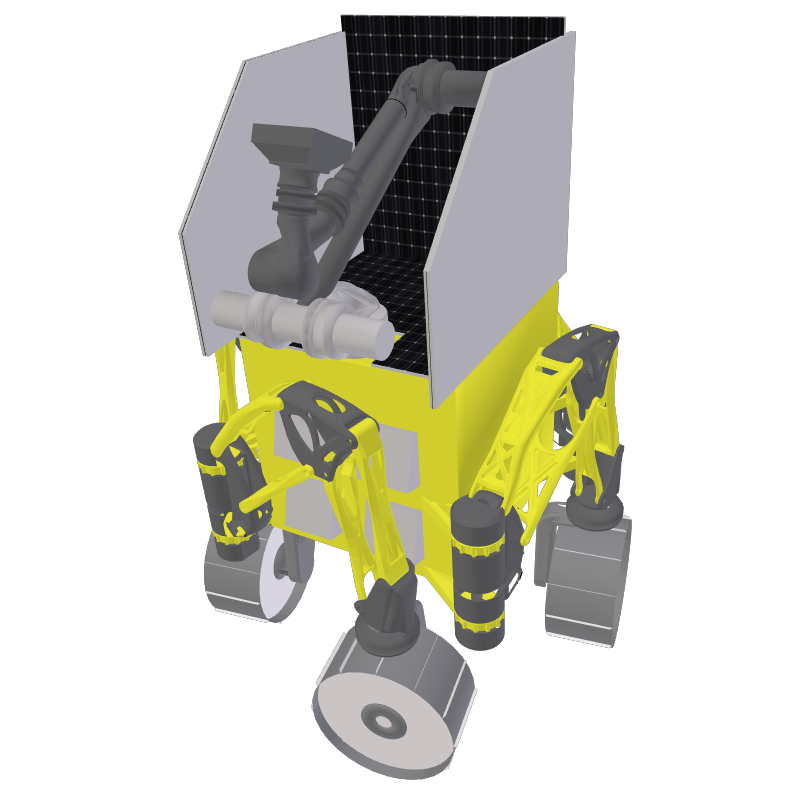
\includegraphics[height=\graphicsHeight]{sections/design/solar-array/images/ismenius-cavus-stowed.png}
  		\subcaption{Folded on stowed rover}
		\label{fig:sub:solar-array-on-rover-for-ismenius-cavus-stowed}
    \end{subfigure}\hfill
    \begin{subfigure}[t]{\subfigureWidth}
        \centering
        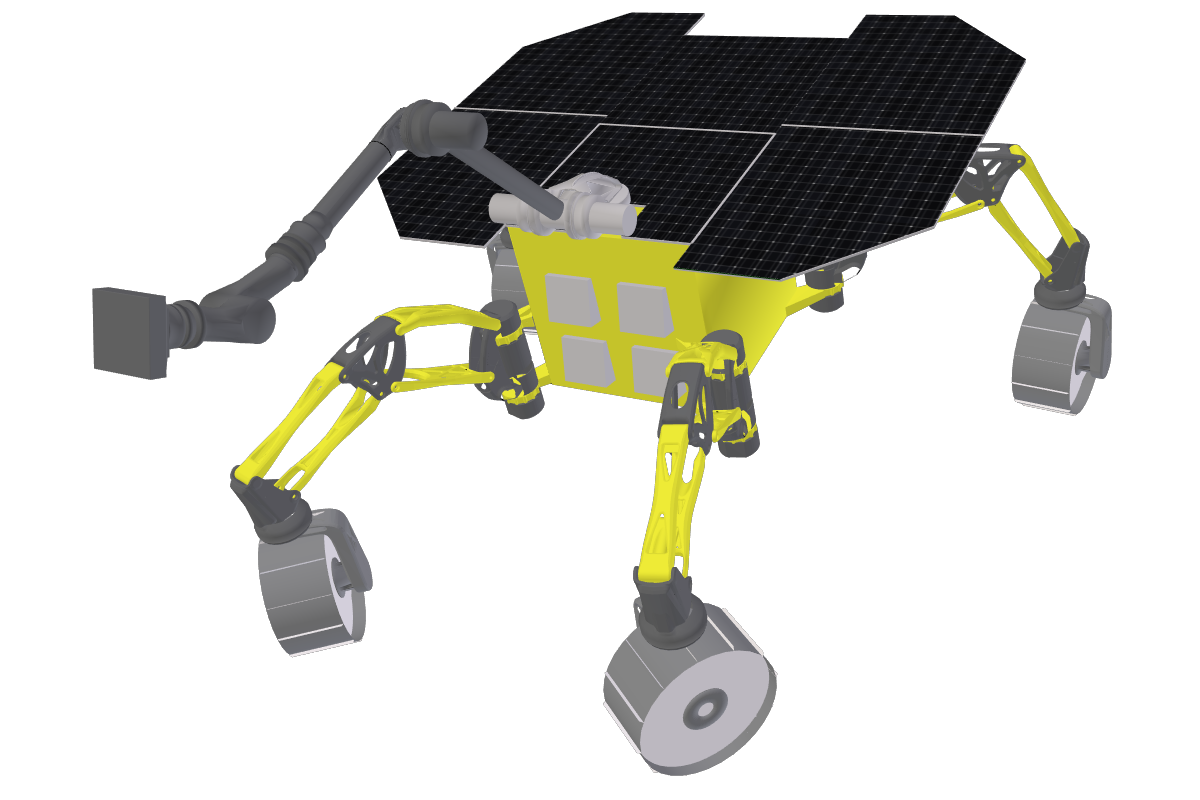
\includegraphics[height=\graphicsHeight]{sections/design/solar-array/images/ismenius-cavus-10deg-pitch.png}
  		\subcaption{Deployed on rover with \SI{10}{\degree} pitch forward}
		\label{fig:sub:solar-array-on-rover-for-ismenius-cavus-deployed}
	\end{subfigure}\\[0.8ex]
    \caption[Solar array on rover for Ismenius Cavus deployment]
            {\ac{SA} on rover for Ismenius Cavus deployment.}
    \label{fig:solar-array-on-ismenius-cavus-chaos}
\vspace{-2ex}
\end{figure}

\clearpage
The unfolded \ac{SA} panel layouts are shown in \refFig{fig:solar-array-layouts-for-missions-sites}. The \ac{SA} at Iani Chaos consists of four panels whereas a six panel design is used at Ismenius Cavus. The bow panels require a cut to accomodate the base of the rover's robotic arm.

\vspace{0.5cm}

\begin{figure}[h]
\captionsetup[subfigure]{justification=centering}
\vspace{-2ex}
	\centering
    %% setup sizes
    \setlength{\subfigureWidth}{0.50\textwidth}
    \setlength{\graphicsHeight}{53mm}
    %% kill hyper-link highlighting
    \hypersetup{hidelinks=true}%
    %% the figures
    \begin{subfigure}[t]{\subfigureWidth}
        \centering
        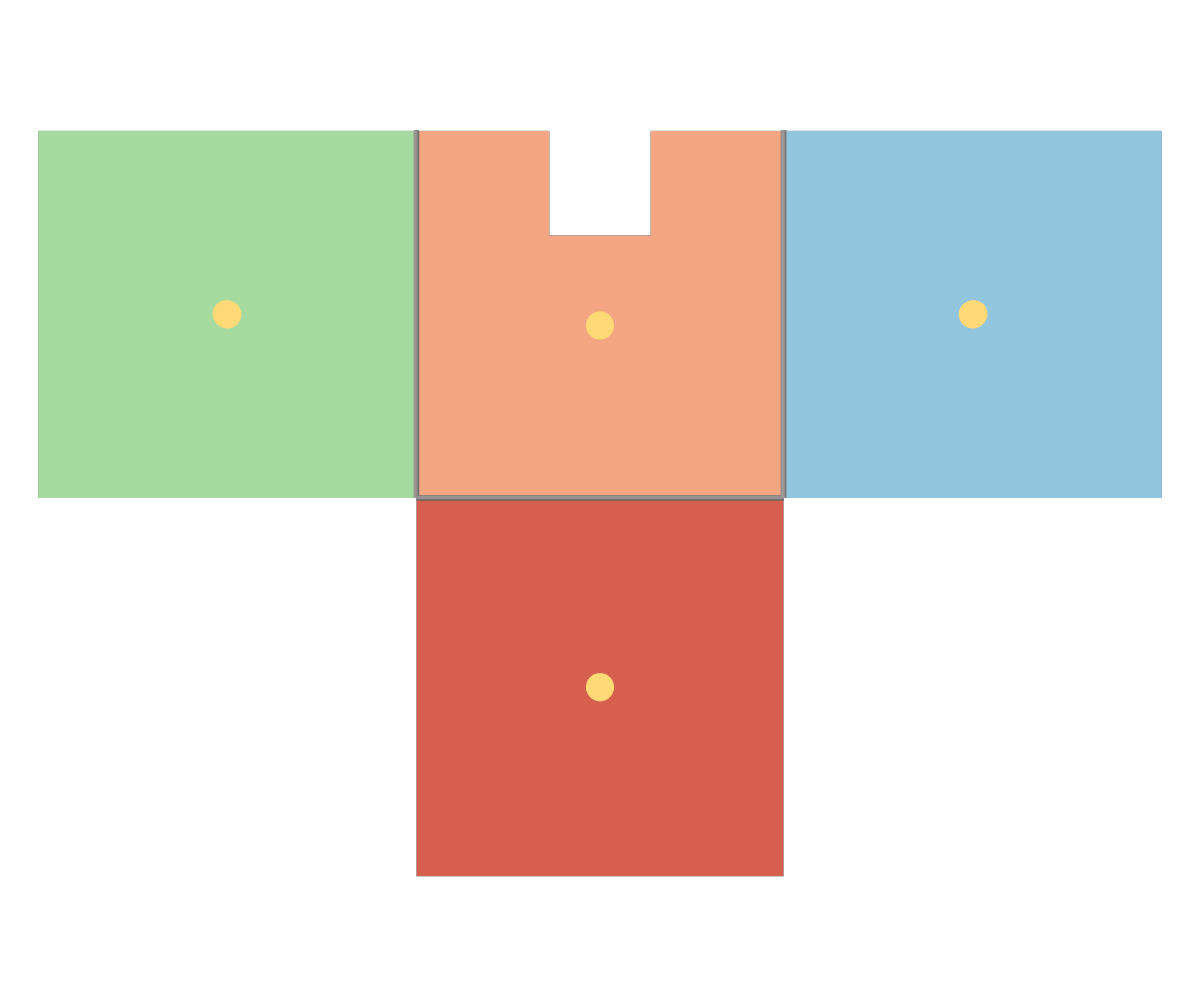
\includegraphics[height=\graphicsHeight]{sections/design/solar-array/images/solar_array_layout_iani_chaos.png}
  		\subcaption{Iani Chaos, \ac{SA} area = \SI{1.7}{m^{2}}}
		\label{fig:sub:solar-array-layouts-for-iani-chaos}
    \end{subfigure}\hfill
    \begin{subfigure}[t]{\subfigureWidth}
        \centering
        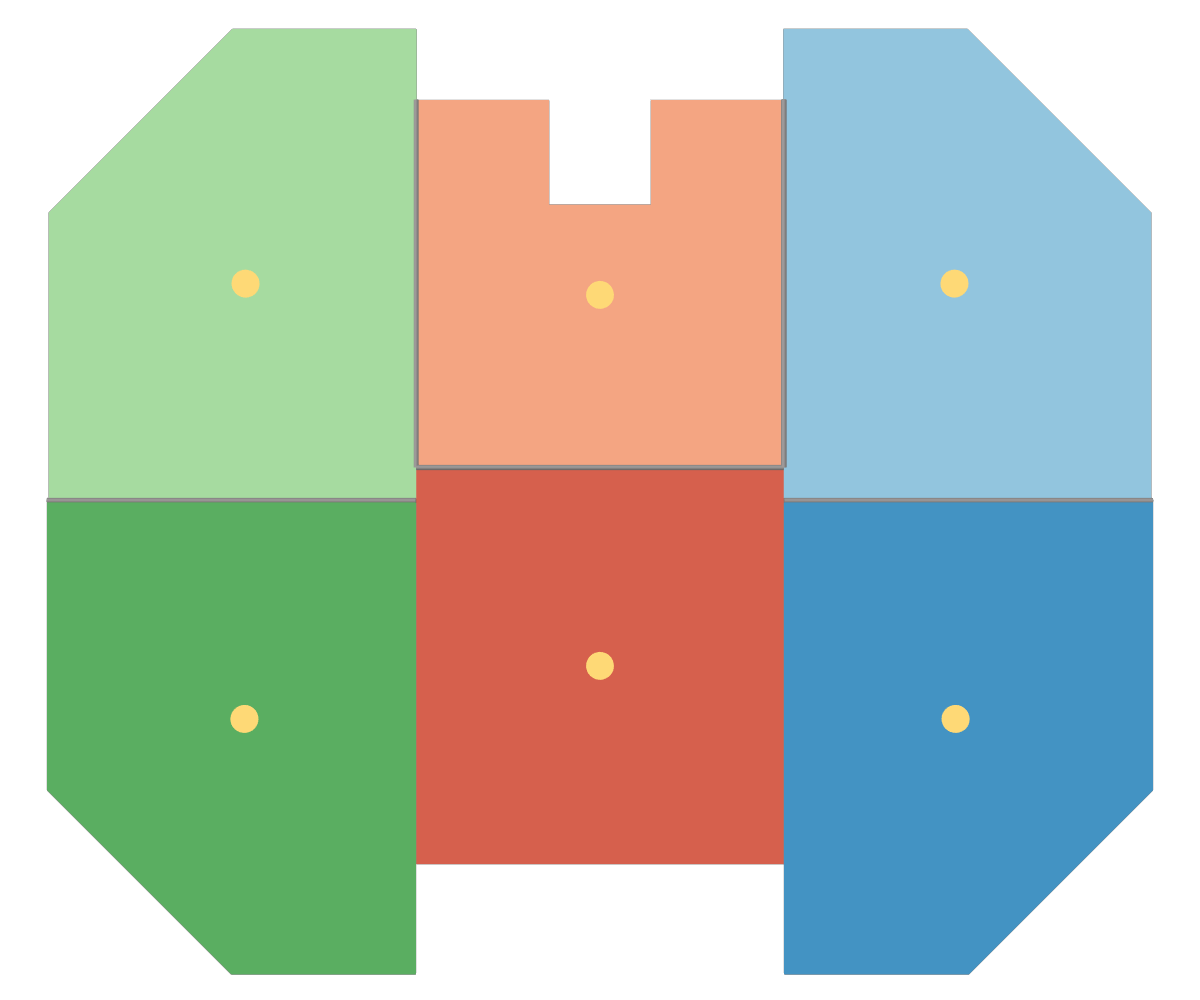
\includegraphics[height=\graphicsHeight]{sections/design/solar-array/images/solar_array_layout_ismenius_cavus.png}
  		\subcaption{Ismenius Cavus, \ac{SA} area = \SI{2.8}{m^{2}}}
		\label{fig:sub:solar-array-layouts-for-ismenius-cavus}
	\end{subfigure}\\[0.8ex]
    \caption[Solar array layouts]
            {\ac{SA} layouts. Green and blue panels are located on the rover's port and starboard, respectively. Port bow and stardboard bow panels are indicated by lighter colors than those on the rover's port quarter and starboard quarter. Light red indicates bow panels which rest over the rover's body. Darker red panels are located on the rover's stern. The yellow dots represent the \ac{CoM} for each panel.}
    \label{fig:solar-array-layouts-for-missions-sites}
\vspace{-2ex}
\end{figure}

\vspace{0.5cm}

Round and diagonal edges negatively affect solar cell packing efficiency and are thus avoided. However, a trade-off is made at Ismenius Cavus due to the large coverage area of the panels and in light of \ref{itm:dd:cog}. Diagonal corners are used for the port and starboard panels to reduce the wingspan of the solar array while preserving the \ac{CoG} within the stowed rover's body and to reduce the panel \ac{CoM} misalignments once deployed. Further \ac{CoG} analysis is required for both configurations with respect to the stern and quarter panels when operating the rover's manipulator arm. This could result in shifting the position of the port and starboard panels. The surface areas and masses of each panel are presented in Table \ref{tab:solar-panel-surface-areas}. Masses were determined from \ref{itm:ass:sa_surface_density} with \ac{SA} surface density of \SI{3.7}{kg.m^{-2}}.

\vspace{0.5cm}

\begin{table}[h]
\footnotesize
\centering
\caption{Solar panel surface areas and mass for mission site solar arrays.}
\label{tab:solar-panel-surface-areas}
\begin{tabular}{l|c|c|c|c|}
\cline{2-5}
\textbf{} & \multicolumn{2}{c|}{\textbf{Iani Chaos}} & \multicolumn{2}{c|}{\textbf{Ismenius Cavus}} \\ \cline{2-5}
 & \textbf{Surface Area {[}m2{]}} & \textbf{Mass {[}kg{]}} & \textbf{Surface Area {[}m2{]}} & \textbf{Mass {[}kg{]}} \\ \hline
\multicolumn{1}{|l|}{{\color[HTML]{A6DBA0} \textbf{Port bow}}} & {\color[HTML]{A6DBA0} \textbf{0.44}} & {\color[HTML]{A6DBA0} \textbf{1.63}} & {\color[HTML]{A6DBA0} \textbf{0.50}} & {\color[HTML]{A6DBA0} \textbf{1.85}} \\ \hline
\multicolumn{1}{|l|}{{\color[HTML]{5AAE61} \textbf{Port quarter}}} & {\color[HTML]{5AAE61} \textbf{-}} & {\color[HTML]{5AAE61} \textbf{-}} & {\color[HTML]{5AAE61} \textbf{0.50}} & {\color[HTML]{5AAE61} \textbf{1.85}} \\ \hline
\multicolumn{1}{|l|}{{\color[HTML]{F4A582} \textbf{Bow}}} & {\color[HTML]{F4A582} \textbf{0.38}} & {\color[HTML]{F4A582} \textbf{1.41}} & {\color[HTML]{F4A582} \textbf{0.38}} & {\color[HTML]{F4A582} \textbf{1.41}} \\ \hline
\multicolumn{1}{|l|}{{\color[HTML]{D6604D} \textbf{Stern}}} & {\color[HTML]{D6604D} \textbf{0.44}} & {\color[HTML]{D6604D} \textbf{1.63}} & {\color[HTML]{D6604D} \textbf{0.42}} & {\color[HTML]{D6604D} \textbf{1.55}} \\ \hline
\multicolumn{1}{|l|}{{\color[HTML]{92C5DE} \textbf{Starboard bow}}} & {\color[HTML]{92C5DE} \textbf{0.44}} & {\color[HTML]{92C5DE} \textbf{1.63}} & {\color[HTML]{92C5DE} \textbf{0.50}} & {\color[HTML]{92C5DE} \textbf{1.85}} \\ \hline
\multicolumn{1}{|l|}{{\color[HTML]{4393C3} \textbf{Starboard quarter}}} & {\color[HTML]{4393C3} \textbf{-}} & {\color[HTML]{4393C3} \textbf{-}} & {\color[HTML]{4393C3} \textbf{0.50}} & {\color[HTML]{4393C3} \textbf{1.85}} \\ \hline
\multicolumn{1}{|r|}{\textbf{Total}} & \textbf{1.7} & \textbf{6.30} & \textbf{2.8} & \textbf{10.36} \\ \hline
\end{tabular}
\end{table}



\clearpage
\subsection{Mechanisms}
Solar panel deployment sequences are presented in this section. The worst case unfolding is identified with respect to panel mass and traveled rotation distance from which initial motor performance requirements are calculated.

\subsubsection{Deployment Sequence}

\ac{SA} panels deployment at Iani Chaos is straightforward and limited two three unfoldings. Port, bow, and starboard panels are deployed simultaneously while the rover is still in its stowed posture. The sequence is illustrated in \refFig{fig:deployment-sequence-iani-chaos}.

\vspace{0.5cm}

\begin{figure}[h]
\captionsetup[subfigure]{justification=centering}
\vspace{-2ex}
	\centering
    %% setup sizes
    \setlength{\subfigureWidth}{0.32\textwidth}
    \setlength{\graphicsHeight}{30mm}
    %% kill hyper-link highlighting
    \hypersetup{hidelinks=true}%
    %% the figures
	\begin{subfigure}[t]{\subfigureWidth}
        \centering
		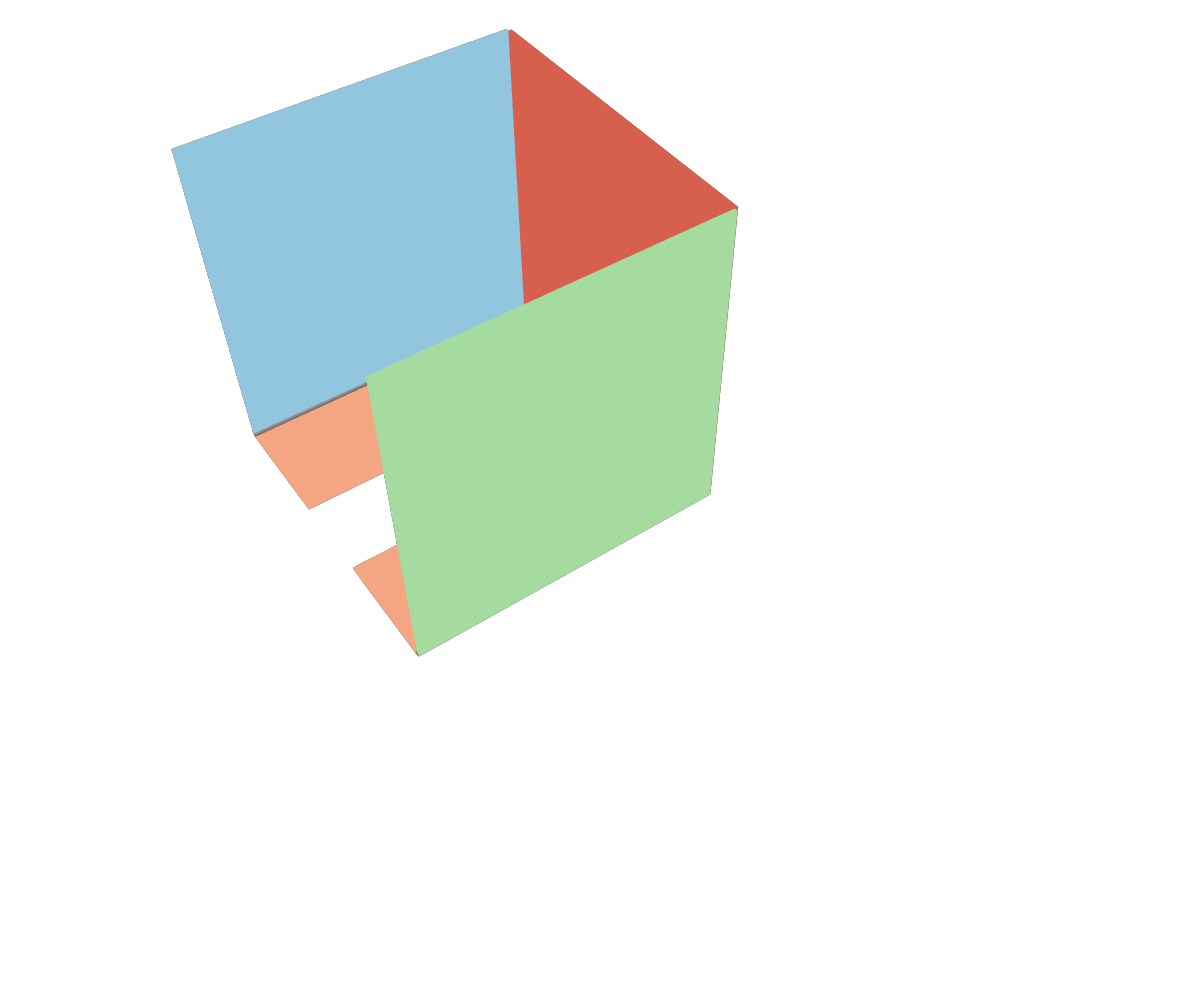
\includegraphics[height=\graphicsHeight]{sections/design/solar-array/images/deployment/iani-chaos/solar_array_deployment_iani_chaos_000.png}
		\subcaption{Folded}
		\label{fig:sub:deployment-sequence-iani-chaos-stowed}
	\end{subfigure}\hfill
	\begin{subfigure}[t]{\subfigureWidth}
        \centering
		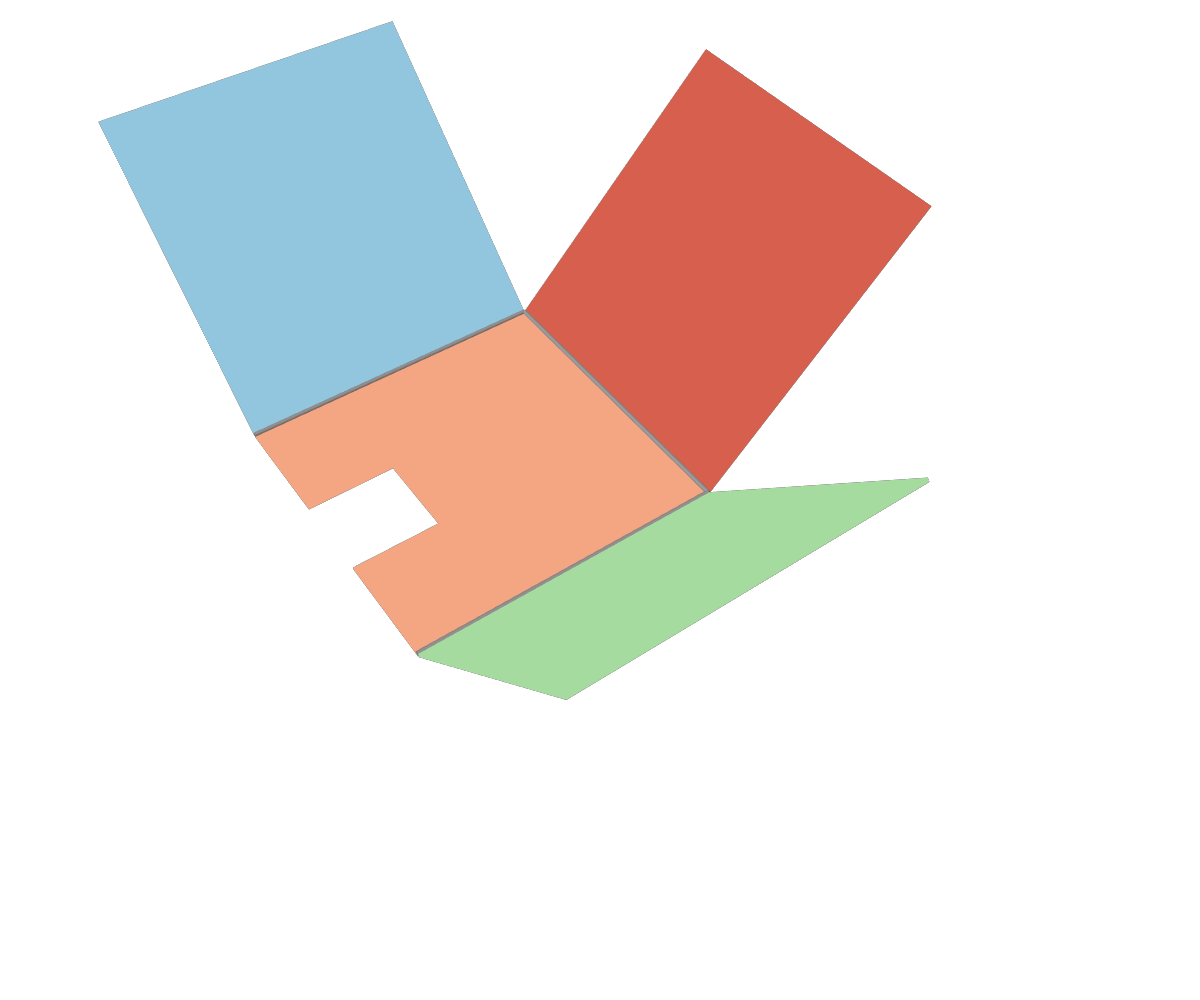
\includegraphics[height=\graphicsHeight]{sections/design/solar-array/images/deployment/iani-chaos/solar_array_deployment_iani_chaos_030.png}
		\subcaption{Mid-deployment}
		\label{fig:sub:deployment-sequence-iani-chaos-mid}
	\end{subfigure}\hfill
    \begin{subfigure}[t]{\subfigureWidth}
        \centering
		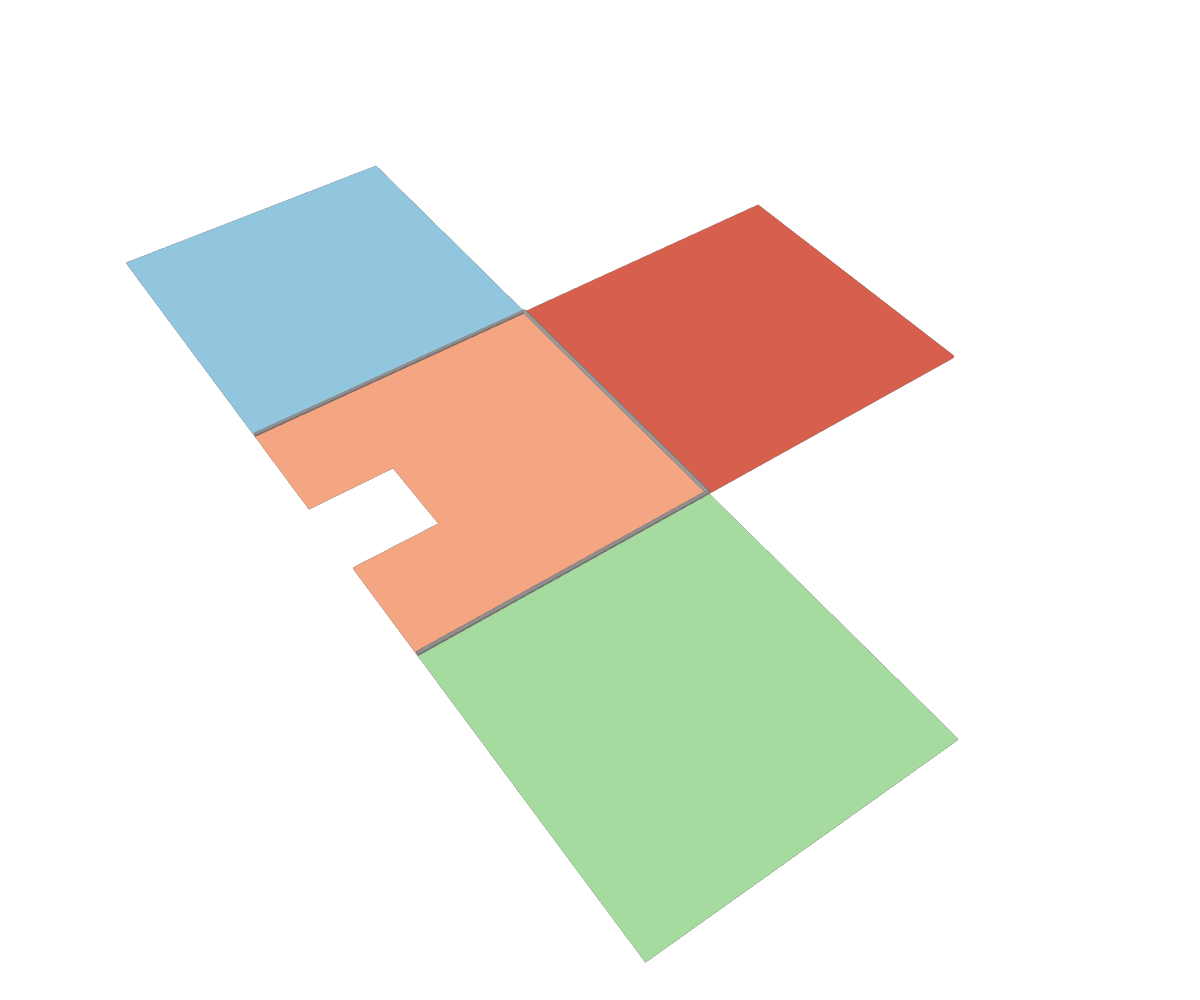
\includegraphics[height=\graphicsHeight]{sections/design/solar-array/images/deployment/iani-chaos/solar_array_deployment_iani_chaos_060.png}
		\subcaption{Deployed}
		\label{fig:sub:deployment-sequence-iani-completed}
	\end{subfigure}
	\caption[Solar array deployment sequence at Iani Chaos]
    {\ac{SA} deployment sequence at Iani Chaos. Total \ac{SA} area is \SI{1.7}{\meter\squared}.}
	\label{fig:deployment-sequence-iani-chaos}
\vspace{-2ex}
\end{figure}

\vspace{0.5cm}

\ac{SA} panels deployment at Ismenius Cavus goes through five unfoldings. The sequence is illustrated in \refFig{fig:deployment-sequence-ismenius-cavus}. The port bow, starboard bow, stern panels are simultenously deployed, completing the first three out of the five unfoldings. The remaining two unfoldings deploy the port quarter and starboard quarter panels.

\vspace{0.5cm}

\begin{figure}[h]
\captionsetup[subfigure]{justification=centering}
\vspace{-2ex}
	\centering
    %% setup sizes
    \setlength{\subfigureWidth}{0.32\textwidth}
    \setlength{\graphicsHeight}{30mm}
    %% kill hyper-link highlighting
    \hypersetup{hidelinks=true}%
    %% the figures
	\begin{subfigure}[t]{\subfigureWidth}
        \centering
		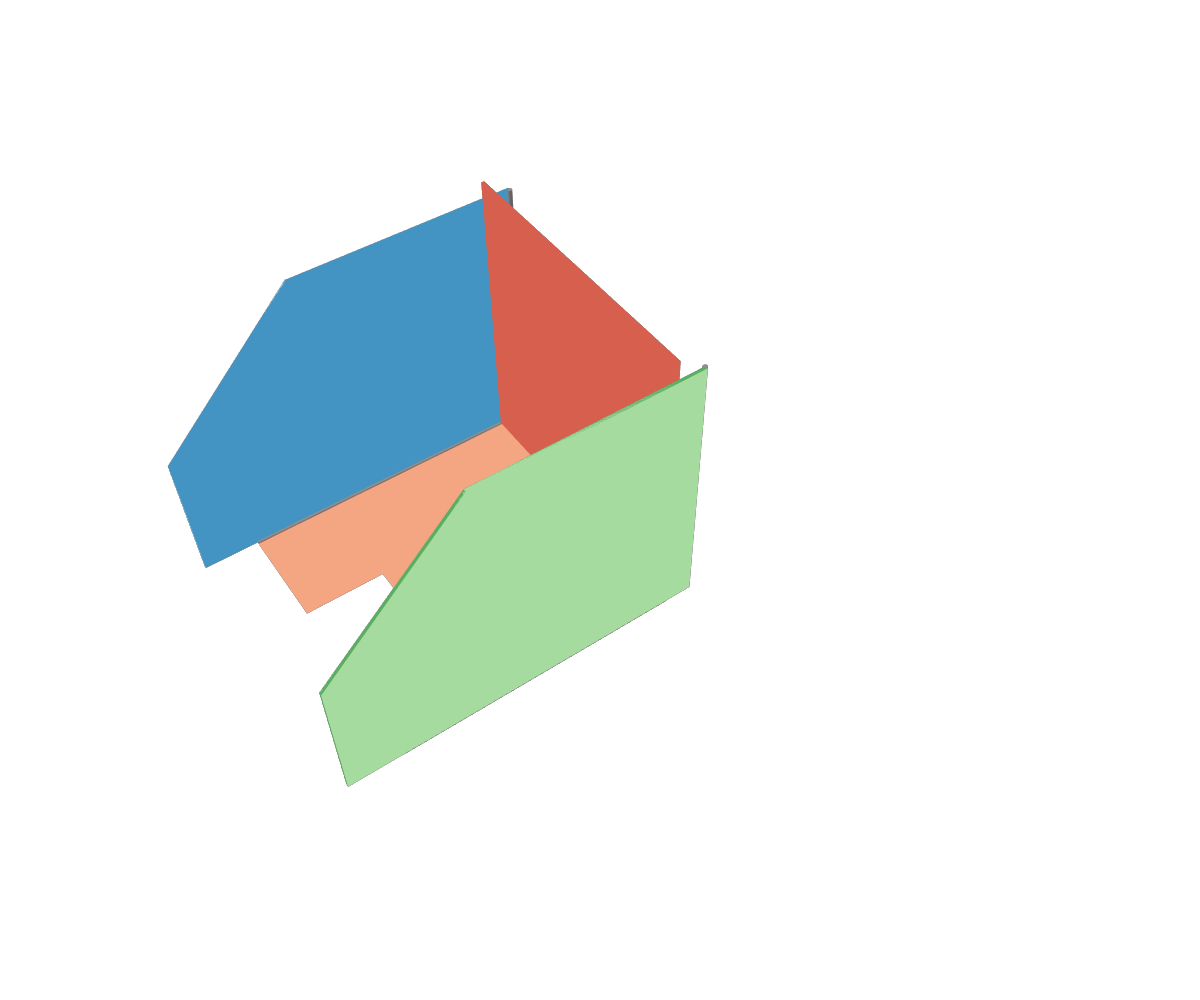
\includegraphics[height=\graphicsHeight]{sections/design/solar-array/images/deployment/ismenius-cavus/solar_array_deployment_ismenius_cavus_000.png}
		\subcaption{Folded panels for stowed posture}
		\label{fig:sub:deployment-sequence-ismenius-cavus-stowed}
	\end{subfigure}\hfill
	\begin{subfigure}[t]{\subfigureWidth}
        \centering
		
\includegraphics[height=\graphicsHeight]{sections/design/solar-array/images/deployment/ismenius-cavus/solar_array_deployment_ismenius_cavus_030.png}
		\subcaption{Port bow, starboard bow, and stern mid-deployment}
		\label{fig:sub:deployment-sequence-ismenius-cavus-mid-bow-and-stern}
	\end{subfigure}\hfill
    \begin{subfigure}[t]{\subfigureWidth}
        \centering
		
\includegraphics[height=\graphicsHeight]{sections/design/solar-array/images/deployment/ismenius-cavus/solar_array_deployment_ismenius_cavus_060.png}
		\subcaption{Port bow, starboard bow, and stern deployed}
		\label{fig:sub:deployment-sequence-ismenius-cavus-full-bow-and-stern}
	\end{subfigure}\\[0.8ex]
%% 2nd row
	\begin{subfigure}[t]{\subfigureWidth}
        \centering
		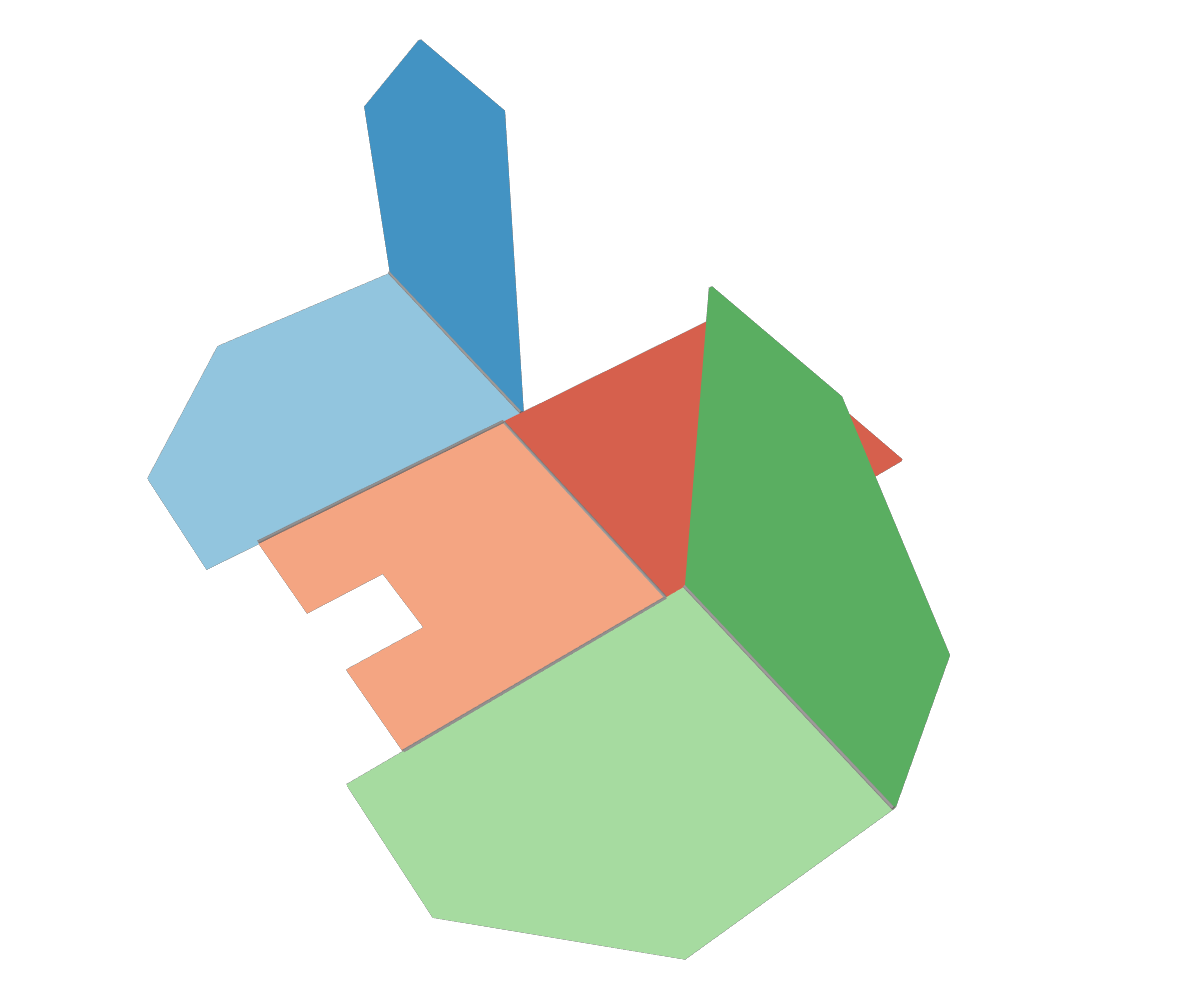
\includegraphics[height=\graphicsHeight]{sections/design/solar-array/images/deployment/ismenius-cavus/solar_array_deployment_ismenius_cavus_100.png}
		\subcaption{Port quarter and starboard quarter mid-deployment}
		\label{fig:sub:deployment-sequence-ismenius-cavus-mid-quarter}
	\end{subfigure}\hspace*{2.5cm}
    \begin{subfigure}[t]{\subfigureWidth}
        \centering
		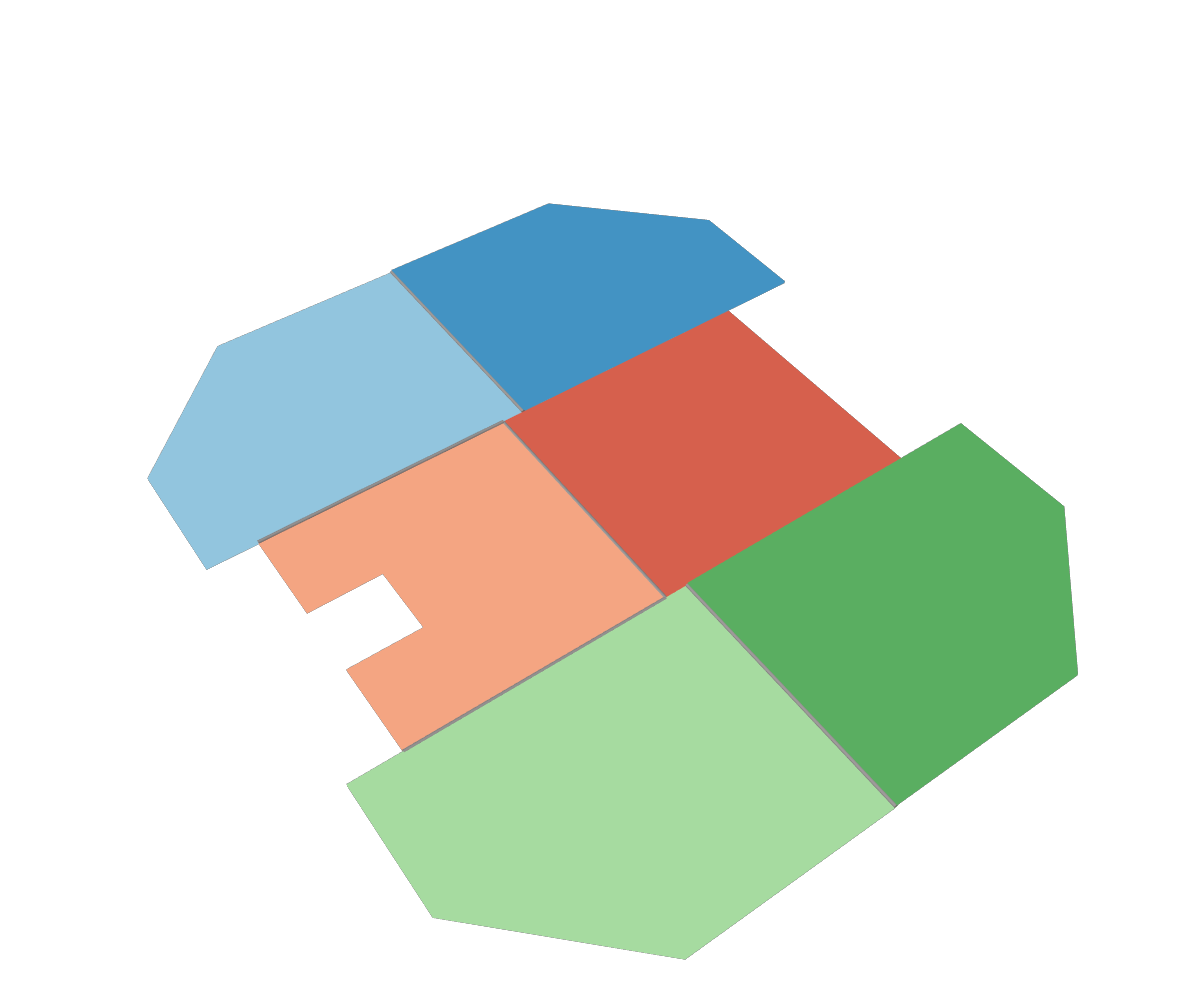
\includegraphics[height=\graphicsHeight]{sections/design/solar-array/images/deployment/ismenius-cavus/solar_array_deployment_ismenius_cavus_130.png}
		\subcaption{Completed deployment}
		\label{fig:sub:deployment-sequence-ismenius-cavus-completed}
	\end{subfigure}
    \caption[Solar array deployment sequence at Ismenius Cavus]
    {\ac{SA} deployment sequence at Ismenius Cavus. Total \ac{SA} area is \SI{2.8}{\meter\squared}.}
	\label{fig:deployment-sequence-ismenius-cavus}
\vspace{-2ex}
\end{figure}

\clearpage
\subsubsection{Motor Requirements}
The worst case motor torque for \ac{SA} deployment occurs when unfolding the port quarter and starboard quarter panels at Ismenius Cavus. This sequence is illustrated from \refFig{fig:sub:deployment-sequence-ismenius-cavus-full-bow-and-stern} to \refFig{fig:sub:deployment-sequence-ismenius-cavus-completed}. The distance between the \ac{CoM} and the rotation joint is shown in \refFig{fig:ismenius-cavus-solar-panel-starboard-quarter-dimensions} and corresponds to $r = \SI{385}{\milli\metre}$.

\vspace{0.25cm}

\begin{figure}[h]
  \captionsetup[subfigure]{justification=centering}
  \centering
  \hypersetup{linkcolor=captionTextColor}
  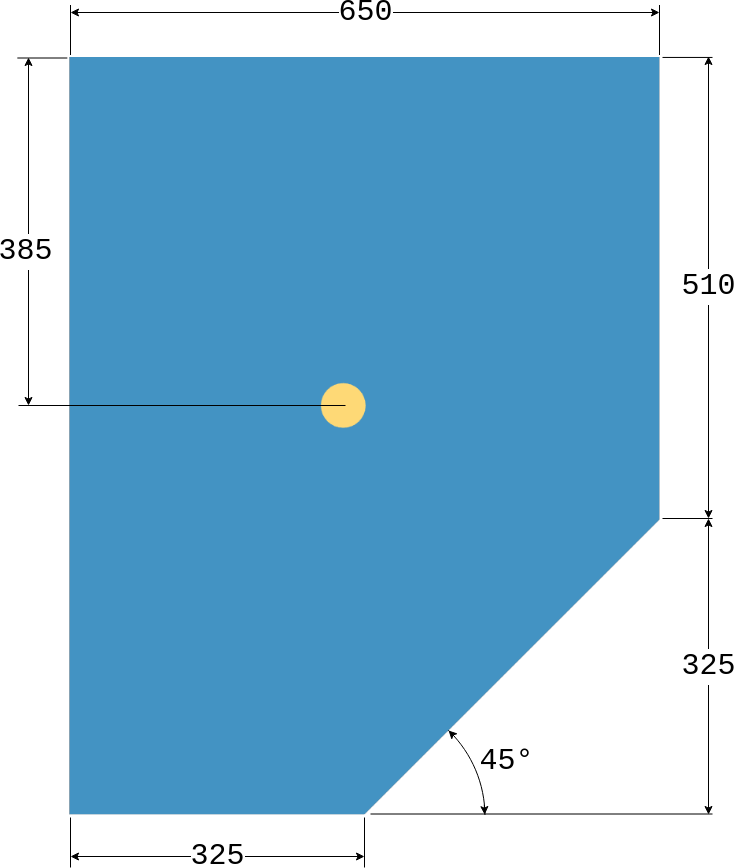
\includegraphics[width=0.45\linewidth]{sections/design/solar-array/images/ismenius-cavus-solar-panel-starboard-quarter.png}\\
  \caption[Dimensions of starboard quarter panel at Ismenius Cavus]
          {Dimensions of starboard quarter panel at Ismenius Cavus. Measurments are in millimeter. The same dimensions apply for the starboard bow, port bow, and port quarter panels. The length between the base of the panel and the \ac{CoM} is also indicated and corresponds to $r = \SI{385}{\milli\metre}$.}
  \label{fig:ismenius-cavus-solar-panel-starboard-quarter-dimensions}
\end{figure}

\vspace{0.25cm}

The acceleration $a$ required to deploy the port quarter and starboard quarter panels must act against the gravity acceleration $g$. For the sake of introducing margins that accounts for Martian environmental factors such as wind loads, the required acceleration $a$ is set to $g_{Earth} = 9.81 \si{ms^{-2}}$. This margin also accounts for imperfections introduced by motor performance degradation factors. Furthermore, sizing motors for an Earth environment reduces design verification and validation costs by eliminating the need for vacuum chamber tests. The panel has a mass of 1.85 \si{\kilo\gram}, thus the required torque $\tau_{torque}$ is:

\begin{align}
  \label{eq:solar-panel-deployment-torque}
  \tau_{torque} &= m \times a \times r\\
                &= 1.85 \times 9.81 \times 0.385\\
                &= 6.99\,\si{\newton\meter}
\end{align}

\clearpage
The \ac{rpm} rotational speed for a deployment rotation duration of \SI{20}{\second} is:

\begin{align}
  \label{eq:solar-panel-deployment-rpm}
  rpm &= \frac{1}{t} \times 60\\
      &= \frac{1}{20} \times 60\\
      &= 3\,{\minute^{-1}}
\end{align}

Transmissions with a 1:30 reduction ratio can be obtained with a planetary gear configuration whereas reduction ratios of 1:100 up to 1:300 are achievable with a harmonic drive. Using a 1:30 transmission will require a motor that must deliver at least 0.23 \si{\newton\meter} of nominal torque and 90 \ac{rpm}. A 1:100 transmission requires a motor with at least $6.99\times\num{e-2}$ \si{\newton\meter} of nominal torque and 300 \ac{rpm}. Finally, a 1:300 transmission requires a motor with at least $2.33\times\num{e-2}$ \si{\newton\meter} of nominal torque and 900 \ac{rpm}.

\subsection{Summary}
\ac{SA} sizing for the worst case power budget of the rover's \textit{Traverse Sol} at optical depth of $\tau = 1$ does not support the use of solar tracking for the purpose of increasing traverse time. This is due to solar irradiance being mostly diffuse at high optical depths when airborn dust is responsible for scattered light. In a dusty atmosphere, an inclined \ac{SA} surface contributes negligeable energy production gains over those obtained with a horizontal configuration. Under certain conditions, these gains are unusable on clear days due to the limited amount of daylight time available for traversing. To resolve this, the \ac{SA} sizing is instead done for the worst case \textit{Hibernation Sol} in which power draws are reduced by introducing \acp{RHU}. Assumptions, requirements, constraints, and design drivers presented in the previous section are considered in the baseline designs from which deployment sequences and motor requirements are presented. The location and stowed posture of the robotic arm should be approached differently so to enable complete folding of the panels over the rover's body. Such a configuration would significantly reduce the vertical span taken up by the stowed rover by approximately 1/3.


\section{Simulation}
\label{sec:Design:Simulation}
The proposed rover redesigns and \ac{SA} configurations for both mission sites are modeled with Blender/Phobos. Phobos is ``an add-on for the open-source 3D modeling software Blender that enables the creation of robot models for use in robot frameworks like ROS and ROCK or in real-time simulations such as MARS'' \citeother{Phobos}. MARS is ``a cross-platform simulation and visualisation tool created for robotics research. It consists of a core framework containing all main simulation components, a GUI (based on Qt), 3D visualization (using OSG) and a physics engine (based on ODE)'' \citeother{MARSSim}. \refFig{fig:simulated-mission-site-ismenius-cavus} shows the robot model loaded on the MARS platform to simulatie mission scenarios using a \ac{HiRISE} \ac{DTM} of a well preserved crater at Ismenius Cavus.  The simulated solar power output data is produced by a \ac{PMS} implemented as part of this thesis which is integrated with the already available robot simulation toolkit.

\begin{figure}[h]
  \captionsetup[subfigure]{justification=centering}
  \centering
  \hypersetup{linkcolor=captionTextColor}
  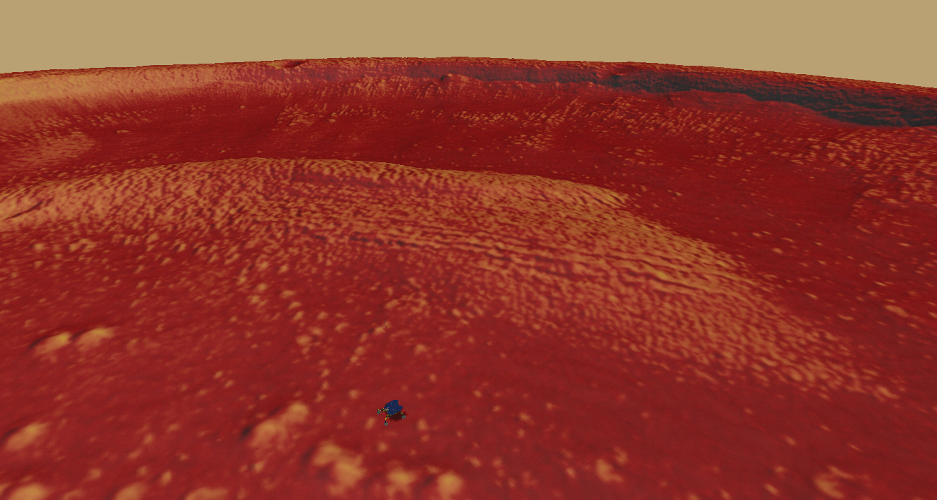
\includegraphics[width=1\linewidth]{sections/design/simulation/images/mars-sim-ismenius-cavus.png}\\
  \caption[Simulation of the rover inside a well preserved crater at Ismenius Cavus]
          {Simulation of the rover inside a well preserved crater at Ismenius Cavus.}
  \label{fig:simulated-mission-site-ismenius-cavus}
\end{figure}

\subsection{Z-Axis Revolutions}

\refFig{fig:simulation-data-rover-revolution-generated-power} and \refFig{fig:simulation-data-rover-revolution-generated-power-polar} are two different representations of the same solar generated power data obtained from commanding the rover to execute a \SI{10}{\degree} forward body-pitch followed by several revolutions around its z-axis. These revolutions result in a sinusoidal generated power variation.

\begin{figure}[h]
  \captionsetup[subfigure]{justification=centering}
  \centering
  \hypersetup{linkcolor=captionTextColor}
  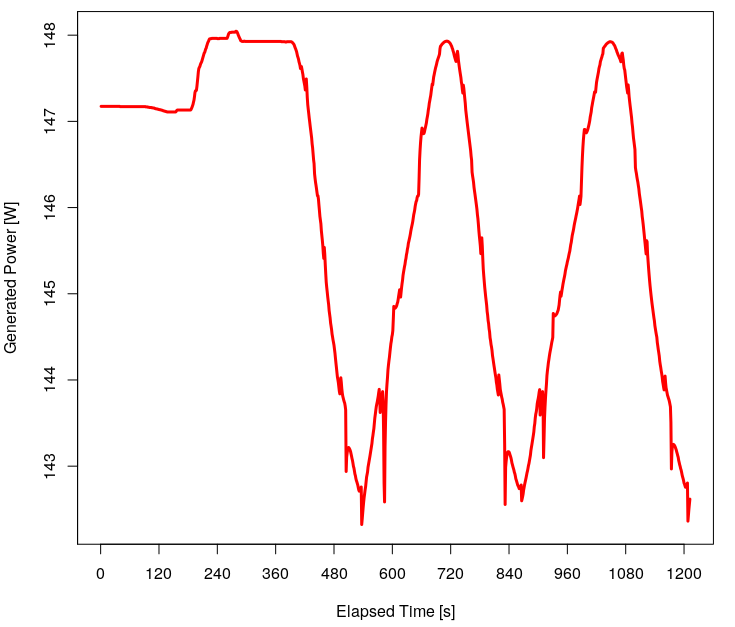
\includegraphics[width=0.5\linewidth]{sections/design/simulation/plots/rover-generated-power.png}\\
  \caption[Power generated by the rover's solar array for multiple revolutions along its z-axis]
          {Power generated by the rover's solar array for multiple revolutions along its z-axis. Simulation conditions is solar noon at Ismenius Cavus.}
  \label{fig:simulation-data-rover-revolution-generated-power}
\end{figure}

In \refFig{fig:simulation-data-rover-revolution-generated-power-polar}, the angle values represent the direction faced by the inclined solar array. Maximum power is generated when the rover's solar panels are facing South towards the equator. Inversely, facing northwards away from the equator genrates the least amount of power.


\begin{figure}[h]
  \captionsetup[subfigure]{justification=centering}
  \centering
  \hypersetup{linkcolor=captionTextColor}
  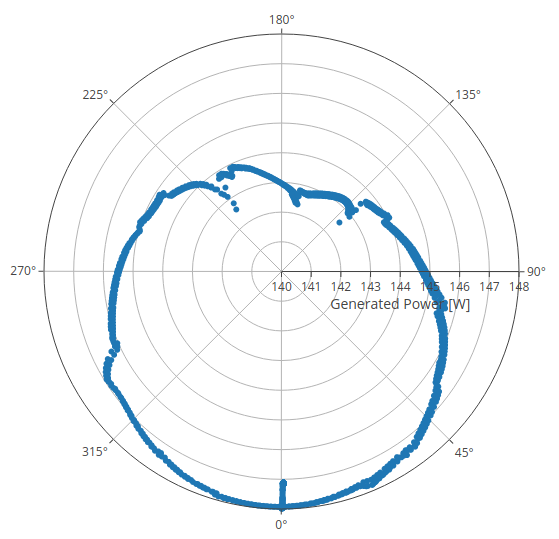
\includegraphics[width=0.4\linewidth]{sections/design/simulation/plots/rover-revolution-generated-power.png}\\
  \caption[Polar visualization of power generated by the rover's solar array for multiple revolutions along its z-axis]
          {Polar visualization of power generated by the rover's solar array for multiple revolutions along its z-axis. Angle values represent the direction faced by the inclined solar array. \SI{0}{\degree} is South, \SI{90}{\degree} is East, \SI{180}{\degree} is North, and \SI{270}{\degree} is West. Simulation conditions is solar noon at Ismenius Cavus.}
  \label{fig:simulation-data-rover-revolution-generated-power-polar}
\end{figure}

\clearpage
\subsection{Slope Compensation}

\refFig{fig:rover-counter-slope} shows a simulated scenario in which the rover is on a \SI{30}{\degree} inclined slope. The slope's inclination is facing opposite the equator resulting in a worst case power generation. The rover is positioned with a backward body-pitch of \SI{10}{\degree} in order to counter the slope induced forward inclination thus reducing \ac{SA} inclination angle from $\beta=\SI{30}{\degree}$ to $\beta=\SI{20}{\degree}$.

\begin{figure}[h]
  \captionsetup[subfigure]{justification=centering}
  \centering
  \hypersetup{linkcolor=captionTextColor}
  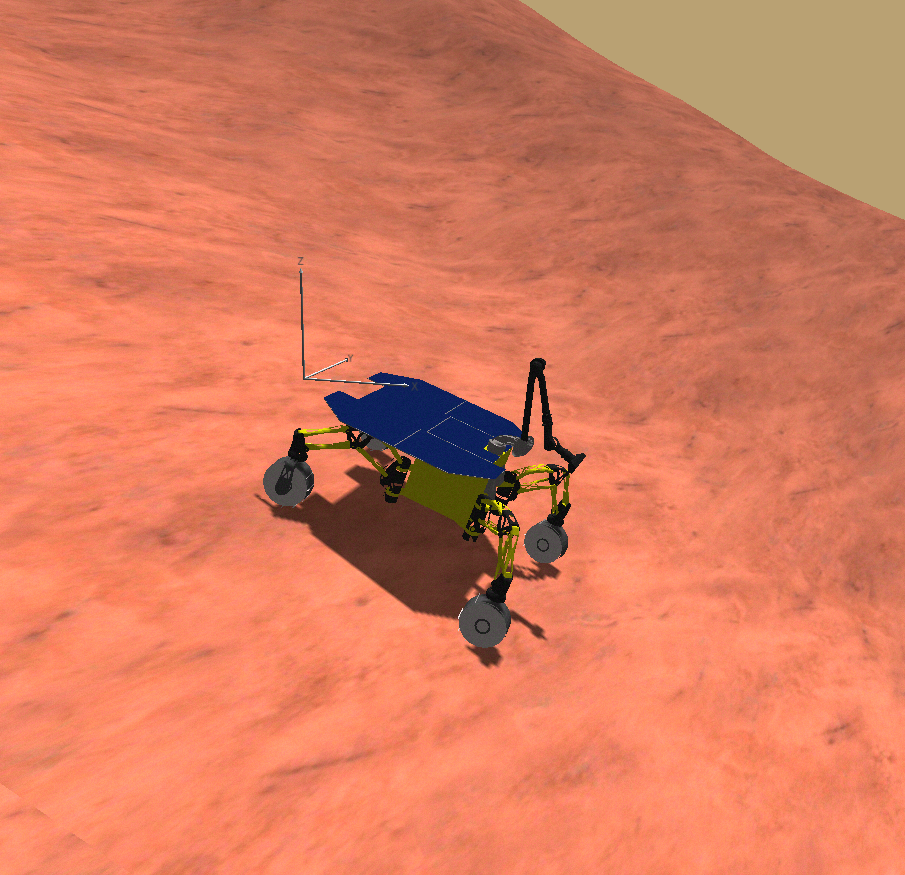
\includegraphics[width=0.4\linewidth]{sections/design/simulation/images/counter-slope.png}\\
  \caption[Simulation of the rover on an inclined slope.]
          {Simulation of the rover on an inclined slope.}
  \label{fig:rover-counter-slope}
\end{figure}

\refFig{fig:rover-counter-slope-measurements} shows solar power outputs for different body-pitch configuration while the rover is on a \SI{30}{\degree} slope. The initial state of the body-pitch is \SI{0}{\degree} follow by two seperate \SI{5}{\degree} forward pitch increments which worsen solar power generation by changing $\beta=\SI{30}{\degree}$ to $\beta=\SI{40}{\degree}$. After which, four separate \SI{5}{\degree} backward pitch decrements are executed, progressively improving power generation as $\beta$ is changed from \SI{40}{\degree} to \SI{20}{\degree}. As a final task, the rover is commanded to drive forward and it encounters uneven terrain which introduces minor fluctuations to the solar power output.

\vspace{0.5cm}

\begin{figure}[h]
  \captionsetup[subfigure]{justification=centering}
  \centering
  \hypersetup{linkcolor=captionTextColor}
  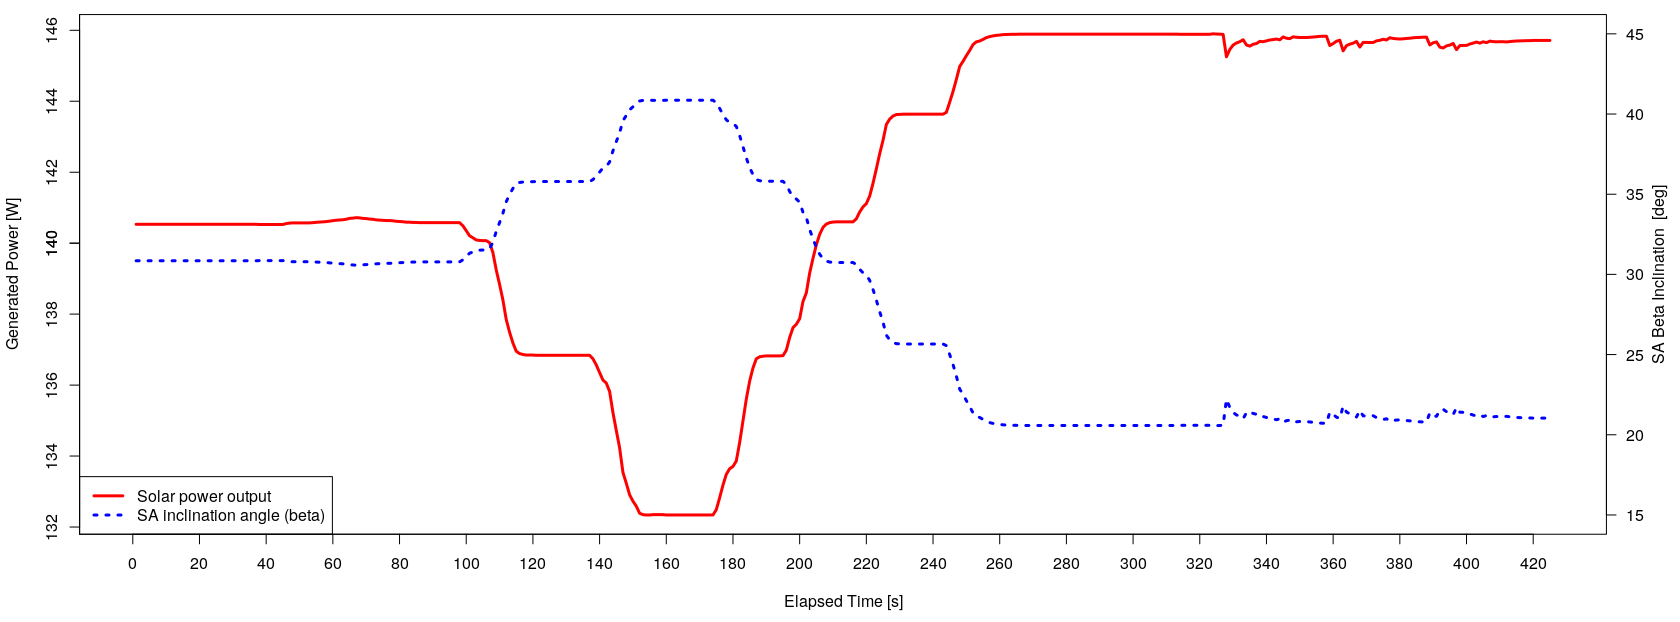
\includegraphics[width=0.9\linewidth]{sections/design/simulation/plots/counter-slope-plot.png}\\
  \caption[Solar power generated on sloped terrain with different SA inclinations.]
          {Solar power generated on sloped terrain with different SA inclinations.}
  \label{fig:rover-counter-slope-measurements}
\end{figure}


\section{Summary and Conclusion}
\label{sec:Design:SummaryAndConclusion}
\todo[inline]{\textbf{TODO:} Write summary and conclusion for this chapter.}
